\chapter{Introducción}
\minitoc{}
\section{Objeto}
El objeto de este proyecto es la implementación de un sistema de \emph{Honeypots} utilizando \emph{containers}. 
Las \emph{Honeypots} existen desde hace bastante tiempo, quizá el software más conocido es \emph{Honeyd}, publicado en 2007.

\emph{Honeyd} (véase \cite{honeynet-lowinteraction}) -junto a otros casos- es  una aplicación de las llamadas \emph{honeypots} de baja interacción, puesto que solo exponían al atacante un entorno limitado
no real y limitado frente a las \emph{honeypots} de alta interacción que permiten al atacante interactuar con la aplicación a investigar, con el sistema operativo
y con todo aquello que pueda ser relevante para el diagnóstico; como puede ser el tráfico de red.

Habitualmente, las \emph{honeypots} de alta interacción eran servidores físicos o virtualizados creados exclusivamente para esta tarea, lo que implicaba
una utilización de recursos en términos de CPU, RAM (en definitiva, en coste económico). Además, se ha de considerar que una \emph{honeypot} (por sus características
y seguridad) tiene altas posibilidades de no desplegarse exactamente en el mismo entorno que el resto de aplicaciones de negocio de una organización y, en caso de hacerlo,
la gestión del riesgo y de las medidas de seguridad aumentaran considerablemente.

Por ello, el despliegue y mantenimiento de \emph{honeypots}  de alta interacción es difícil. Desde la introducción de LXC (Linux Containers) en el \emph{kernel} de Linux que los hizo posible, y
especialmente desde la aparición de Docker, que le dio popularidad y facilito su adopción y explotación.

Un \emph{container} es un método de virtualización para ejecutar múltiples sistemas linux aislados (\emph{containers}) en un servidor que comparte un mismo \emph{kernel} de Linux. Técnicamente, se basa en la utilización
de \emph{cgroups} para limitar y priorizar recursos del sistema (CPU, memoria, I/O...), y de \emph{namespaces}, que limitan la visualización del sistema de los procesos que se ejecutan en el \emph{container}, y que es la técnica que produce el aislamiento. Es importante notar que
frente a otras tecnologías de ``contanerización'' (como \emph{Jails}, \emph{Zones} o, incluso, las máquinas virtuales), los \emph{containers} no tienen entidad propia para el \emph{kernel}, así que un \emph{container} se compone
de una definición de \emph{cgroups} y \emph{namespaces}. 

Se puede considerar un \emph{container} como un \emph{chroot} mejorado o como una máquina virtual ligera (que comparte el mismo \emph{kernel} que el hipervisor). En este sentido
mi interés en \emph{containers} para este proyecto es debido a su eficiente utilización de recursos frente a una máquina virtual y a la facilidad
de crear, mantener y mejorar imágenes de sistema gracias al \emph{tooling} alrededor de imágenes de Docker.

En resumen, el objeto de este proyecto es el de construir una \emph{honeypot} de alta interacción utilizando \emph{containers}.

\section{Alcance}

El presente proyecto tendrá como alcance:
\begin{itemize}
    \item La creación de una sonda que exponga al mundo el servicio que se quiere investigar y que se ejecutará en un \emph{containers}.
    \item La aplicación de las medidas de seguridad de dicha sonda.
    \item El uso de un sistema que guarde las trazas para poder identificar las acciones realizadas en la \emph{honeypot}.
    \item El diseño de un sistema de colección, que recopile las trazas de las sondas y las almacene.
    \item El diseño de un sistema de explotación de datos de dicha colección; en particular de la extracción, transformación y visualización de los mismos.
\end{itemize}

\section{Antecedentes}

% honeypots existentes...
% Kippo, honeyd, honeynet, dionaea 

El objetivo de una \emph{honyepot} es el de aprender y conocer técnicas de los atacantes para poder defenderse aplicando medidas de seguridad.
Debido al coste y complejidad de las \emph{honeypots} de alta interacción, la mayoría de ellas son de baja interacción. A continuación, se examinarán brevemente algunas de ellas:

\begin{enumerate}
    \item \emph{Kippo} (\cite{honeynet-kippo}): una \emph{honeypot} de SSH de baja interacción, implementa el protocolo SSH en un servidor en Python
    lo que le permite extraer información del atacante (contraseña, IP, órdenes ejecutadas...), aunque intenta simular un servidor de SSH real
    se puede diagnosticar que el servidor es una \emph{honeypot} simplemente ejecutando órdenes de sistema.
    \item \emph{Dionaea} (\cite{honeynet-dionaea}): una \emph{honeypot} de baja interacción que simula varias aplicaciones como servidores TFTP, MySQL, HTTP, Memcache etc y expone sus puertos.
    \item \emph{honeyd} (\cite{honeynet-lowinteraction}): una de las primeras \emph{honeypots open source} de baja interacción que puede exponer varios servicios aunque su desarrollo no está activo.
    \item \emph{Dockerpot} (\cite{honeynet-dockpot}): una \emph{honeypot} de alta interacción, basada en \emph{containers} Docker que persigue un objetivo similar al de este proyecto.
    Sin embargo, no se expone directamente un \emph{container}, sino que expone un \emph{proxy} (a lo \emph{kippo}) que implementa el protocolo SSH. Pero a diferencia de \emph{kippo}, se abre otra conexión
    a un servidor SSH real que se ejecuta en un \emph{container}. El \emph{proxy} se encarga de levantar o de parar el \emph{container}, pero solo se para el \emph{container} cuando no hay ninguna conexión activa. Y, si el \emph{container} es comprometido, siguiendo este enfoque, no se parará.
    De manera similar a \emph{Kippo}, es fácil descubrir  que se está atacando una \emph{honeypot} de este tipo, ya que la latencia entre que se inicia la comunicación
    y que se pide la contraseña o se deniega el acceso al servidor SSH, es sensiblemente elevada.
\end{enumerate}

Si hay algo en común en todas ellas que motivó la creación de este proyecto es: que o bien son \emph{honeypots} de baja interacción fácilmente reconocibles
y, por lo tanto, carecen de interés para ataques reales; o bien son de alta interacción pero, para reciclar y/o gestionar el servicio expuesto, siempre hay un \emph{proxy} delante
que se encarga de levantar o de parar el \emph{container}.

\section{Requisitos de diseño}
\label{sec:requisitos-de-disenyo}

Para el diseño de la \emph{honeypot} basada en \emph{containers}, los principios que han regido el proyecto son: la funcionalidad, la seguridad y la viabilidad económica. Y a estos principios, se les ha de sumar la búsqueda de cualidades como la flexibilidad, eficiencia, utilidad y seguridad. ``Flexibilidad'' porque la \emph{honeypot} debe ser capaz de exponer cualquier tipo de servicio requerido. ``Eficiencia'' ya que las sondas y el \emph{backend} deben minimizar el número de servidores necesarios para su explotación. ``Utilidad'' porque las \emph{honeypots} deben exportar información útil. Y, por último, ``seguridad''  en tanto que las \emph{honeypots} y el \emph{backend} deben proveer de medidas de contención frente a los atacantes.

\chapter{Planificación y presupuesto.}
\section{Metodología de desarrollo}

Para la realización del proyecto se ha utilizado un modelo iterativo incremental como enfoque general. Era importante definir
muy bien el conjunto de funcionalidad a incluir y la calidad mínima en cada iteración sin atender a una estimación en fechas. 
Cualquier estimación se realizaba en tallas de camiseta o puntos de historia que miden la complejidad y no la duración de una tarea.

Cabe reseñar que el alumno y desarrollador del proyecto no tiene una dedicación completa al mismo, pudiendo dedicar unas 10 horas semanales
de media al proyecto. Esto tiene impacto en la duración del mismo, puesto que al tiempo inherente a cada tarea hay un tiempo
invertido en recuperar el contexto de la última sesión de trabajo lo cual incrementa la duración del desarrollo del proyecto.


\subsection{Primera iteración: construcción del prototipo.}

La primera iteración se basa en validar la idea del proyecto y evaluar las herramientas que utilizaremos. Para ello se construye
un prototipo creando manualmente una sonda  y se evalua como se extraería información de la misma de manera automatizada.

También se exploran tecnologías para realizar la recolección y construir la API. El resultado de esta iteración se describe en
el capítulo \ref{chapter:analisis-de-soluciones}.

\subsection{Segunda iteración: construcción de las sondas.}

El objetivo de esta iteración es construir las sondas de manera repetible y automatizada asegurando que son estables,
seguras y resistentes y que tenemos los mecanismos necesarios para extraer información de ellas.

En esta etapa se decide:

\begin{itemize}
    \item Construir un sistema similar para las notificaciones de alertas hasta descubrir que \emph{Falco} es liberado, cuando se descarta.
    \item Utilizar \emph{Ansible} para la creación y configuración de las sondas y el resto de servicios de manera automatizada.
    \item Securizar la sonda de ataques y definir el modelo de riesgo de la sonda.
\end{itemize}

\subsection{Tercera iteración: construcción del recolector.}

Con las sondas funcionando, el siguiente paso es la extracción, almacenamiento y procesado de la información que capturan. En esta iteración
se decide utilizar \emph{Elasticsearch} como motor base de datos, se desarrollan \emph{metadata\_extractor} para recolectar y procesar las trazas, y 
la API de registro de sondas (\emph{Sinker Registry API}). 
También se recolectan las alertas utilizando \emph{rsyslog} y se escriben en \emph{Elasticsearch}
con \emph{Filebeat} y \emph{Logstash}.

En el apartado \ref{sec:arquitectura-del-colector} se detalla las razones y el procedimiento seguido para las implementaciones de estas funciones.

\subsection{Cuarta iteración: construcción de la API.}

Con nuestro proceso de extracción, procesado y almacenamiento de datos solo queda trabajar en la explotación y visualización de la misma. En esta iteración
el enfoque es en el de construir una API de clientes \emph{Beekeeper API}, en la sección \ref{sec:arquitectura-api-clientes} se realiza
una descripción completa del sistema.

\subsection{Quinta iteración: redacción de la memoria del proyecto.}

Como dirían los anglosajones \emph{last, but not least}. Con el sistema funcionando y en producción solo queda la redacción de esta memoria
para dar por acabado el presente PFC.

\section{Calendarización}

En el cuadro \ref{tab:calendarizacion-pfc} puede verse el tiempo invertido en cada iteración. No se puede observar el desfase 
entre la estimación y el coste invertido porque nunca se ha estimado la duración de las tareas, solo se ha estimado la complejidad
de las mismas.

Atendiendo a ese criterio, la calendarización cuadra con la estimación de \emph{complejidad} del proyecto, las fases de prototipo y construcción
de la sonda serían las más complejas puesto que se alejan más del dominio de conocimiento del desarrollador del proyecto.

\begin{table}[h]
    \centering
    \begin{tabular}[!h]{|c|l|l|c|}
    \hline
    \thead{Iteración} & \thead{Inicio} & \thead{Fin} &  \thead{Horas invertidas aprox} \\
    \hline
    \textbf{1ª} & 15/2/2016 & 21/5/2016 & 140 horas \\
    \hline
    \textbf{2ª} & 21/5/2016 & 20/5/2017 & 520 horas \\
    \hline
    \textbf{3ª} & 21/5/2017 & 21/7/2017 & 90 horas  \\
    \hline
    \textbf{4ª} & 21/7/2017 & 08/8/2017 & 20 horas  \\
    \hline
    \textbf{5ª} & 08/8/2017 & 03/9/2017 & 40 horas \\
    \hline
    \end{tabular}
    \caption{\label{tab:calendarizacion-pfc} Calendarización del proyecto }
    \end{table}

\section{Recursos inventariables}

Los recursos de \emph{hardware} utilizados para la elaboración del presente proyecto y su puesta en marcha, se detallan a continuación:

\begin{itemize}
    \item Servidor con gran capacidad de almacenamiento y procesamiento.
    \begin{itemize}
        \item CPU: Intel(R) Core(TM) i7-3770 CPU @ 3.40GHz
        \item RAM: 4 x Kingston DDR3 8GiB (32 GiB)
        \item Disco: RAID 1 por software de 2 discos TOSHIBA DT01ACA300 de 3TiB
    \end{itemize}

    \item Servidor para sonda en Alemania en el proveedor \emph{Vultr} virtualizado.
    \begin{itemize}
        \item CPU: 1 vCore
        \item RAM: 1GiB RAM.
        \item Disco: 20GiB de disco
    \end{itemize}

    \item Servidor para sonda en Holanda en el proveedor \emph{Digital Ocean} virtualizado.
    \begin{itemize}
        \item CPU: 1 vCore Intel(R) Xeon(R) CPU E5-2630L 0 @ 2.00GHz.
        \item RAM: 1GiB RAM.
        \item Disco: 30GiB de disco.
    \end{itemize}

    \item Servidor para \emph{PKI} y control en Londres en el proveedor \emph{Digital Ocean} virtualizado.
    \begin{itemize}
        \item CPU: 1 vCore Intel(R) Xeon(R) CPU E5-2630L 0 @ 2.00GHz.
        \item RAM: 1GiB RAM.
        \item Disco: 30GiB de disco.
    \end{itemize}

    \item Registro DNS de dominio para la \emph{honeypot} y la API de clientes en \emph{Amazon Web Services} y monitorización
    externa del servicio.

\end{itemize}


\section{Presupuesto}

Para el presupuesto debemos desglosar dos conceptos fundamentales:

\begin{itemize}
    \item El coste en \emph{hardware} y servicios.
    \item El coste del personal durante el tiempo de desarrollo y mantenimiento.
\end{itemize}

Si consideramos el desarrollo \emph{acabado}, se necesitará un número de horas del personal para el mantenimiento del proyecto, 
incluyendo actualizaciones de seguridad de los servidores, gestión de incidentes, arreglo de errores etc.

En cuanto al personal. tanto para el desarrollo como para el mantenimiento del mismo necesitamos un perfil \emph{DevSecOps}. Dicho de otro modo
alguien capaz de involucrarse indistintamente en tareas de codificación, administración de servidores y tareas de seguridad. 

En el convenio colectivo de empresas de ingeniería (véase \cite{boe-convenio}) se detalla que un licenciado y/o analista cobrará un sueldo bruto de 
23.618,28 € al año. El perfil previamente descrito entraría dentro de dicha categoría profesional cifrándose el precio/hora en
14 € / hora. 

El cuadro \ref{tab:costes-totales} incluye los costes totales del proyecto y sus conceptos hasta la fecha de redacción de la presente
memoria, no se incluye el coste de mantenimiento por parte del personal. Es el alumno el que desarrolla las labores de personal, se incluyen
los costes aproximados para valorar la dimensión económica de ampliar el equipo técnico.

\begin{table}[h]
    \centering
    \begin{tabular}[!h]{|c|c|c|}
    \hline
    \thead{Concepto} & \thead{Unidades} & \thead{precio/mes}  \\
    \hline
    Servidor en \emph{Hetzner} para recolector & 1 & 41,69 € \\
    \hline
    Servidor en \emph{Vultr} para sonda & 1 & 12 € \\
    \hline
    Servidor en \emph{Digital Ocean} para sonda & 1 & 12 € \\
    \hline
    Servidor en \emph{Digital Ocean} para \emph{PKI} y control & 1 & 12 € \\
    \hline
    Registro DNS y monitorización externa en \emph{AWS} & 1 & 10 € \\
    \hline
    \textbf{Total / mes} & - & \textbf{87,69 €} \\
    \hline
    \end{tabular}
    \caption{\label{tab:presupuesto-mensual} Tabla de costes mensual }
    \end{table}


    \begin{table}[h]
        \centering
        \begin{tabular}[!h]{|c|c|}
        \hline
        \thead{Concepto} & \thead{Precio}  \\
        \hline
        Coste del servidor para prototipo (3 meses) & 30 € \\
        \hline
        Coste de \emph{hardware} del proyecto (15 meses) & 87,69 x 15 = 1315,35 €  \\
        \hline
        Coste de desarrollo del proyecto & 810 horas x 14 €/hora =  11340 € \\
        \hline
        \textbf{Total} &  \textbf{12685,35 €} \\
        \hline
        \end{tabular}
        \caption{\label{tab:costes-totales} Tabla de costes del proyecto hasta fecha actual }
        \end{table}
    

    
    
    
    
    
    

\chapter{An\'alisis de soluciones}
\label{chapter:analisis-de-soluciones}
\minitoc{}


\section{An\'alisis de soluciones para la sonda}
\label{sec:analisis-sonda}


Lo más relevante de la sonda es la capacidad de extraer información de ella a nivel de instrumentación. Cada proceso (y cabe recordar que un \emph{container} en Linux es un proceso dentro de un \emph{namespace} con un \emph{cgroup} asociado) es gestionado, controlado
y auditado por el \emph{kernel}.

Por ello, es interesante explorar si a través de alguna interfaz del \emph{kernel} es posible instrumentar nuestra \emph{honeypot}. A la hora de exponer nuestro servicio, se hará utilizando
un \emph{container}. Existen diversas tecnologías para utilizar \emph{containers} en Linux. Citándolos de más a menos antigüedad, se puede utilizar LXC, \emph{Docker}, \emph{LXD} o \emph{rkt}.

\emph{LXC}, \emph{LXD} y \emph{rkt} comparten que su objetivo es el de proporcionar una \emph{lightweight-VM}; un entorno donde se pueden lanzar varios procesos y aplicaciones a la VM
pero sin la necesidad de cargar un \emph{kernel} independiente y los costes extra que una VM supone (y perdiendo las garantías de aislamiento que también provee).

\emph{Docker}, sin embargo, promueve una filosofía en la que cada \emph{container} debería albergar idealmente un solo proceso o aplicación.

Hay varias diferencias entre estas alternativas: \emph{LXC} y \emph{LXD} proveen de herramientas para crear un \emph{container} ``manualmente'' entrando en el \emph{container} y lanzando los procesos. Por su parte, \emph{Docker} y \emph{rkt}
lanzan \emph{containers} utilizando imágenes. Una imagen no es más que una descripción en un lenguaje acerca de qué contendrá el \emph{container}, órdenes a lanzar para construir el \emph{container} y el punto de entrada (la orden que se lanzará al lanzar el \emph{container}) del mismo.

Además, los \emph{containers} construidos con \emph{Docker} y \emph{rkt} son inmutables. Cada imgen define varias capas de almacenamiento (véase \cite{docker-storage}) que se van apilando
para construir el sistema de archivos y como última capa se añade una con permisos de lectura/escritura para permitir el almacenamiento temporal necesario para lanzar
la mayoría de órdenes.

Aunque cualquiera de las tecnologías de ``containerización'' explicadas previamente podrían ser utilizadas para el fin y objetivo propuesto, \emph{Docker} tiene una amplia acogida como la herramienta de ``containerización''
y hay muchísimas herramientas disponibles que, al final, suponen la utilización de \emph{Docker}. Por ello, se escoge esta tecnología para construir nuestros \emph{container}.

\subsection{Instrumentación de los \emph{containers}}
\label{subsec:instrumentacion-containers}

Cuando se habla de instrumentación de procesos en Linux, generalmente, lo que se persigue es obtener información de:
\begin{enumerate}
    \item \emph{System calls}: peticiones que realiza nuestro proceso al \emph{kernel} como leer un fichero o abrir una conexión.
    \item \emph{Kernel function calls}:funciones que se reclamarán en el \emph{kernel} para satisfacer una \emph{syscall}.
    \item \emph{Eventos}: eventos que se han definido en \emph{userspace} o dentro del \emph{kernel}.
\end{enumerate}

Para obtener esta información hay diversas fuentes dentro del \emph{kernel}:

\begin{enumerate}
    \item \emph{kprobes}: el \emph{kernel} modifica las instrucciones en ensamblador en tiempo de ejecución para activar la instrumentación. Si se trata
    de \emph{kprobes}, las funciones a instrumentar son parte del \emph{kernel}. 
    \item \emph{uprobes}: similar a \emph{kprobes} pero para funciones en espacio de usuario como \emph{malloc}.
    \item \emph{tracepoints}: a diferencia de un \emph{kprobe} o \emph{uprobe}, un \emph{tracepoint} se define en el código fuente y se genera en tiempo de compilación, pudiendo ser activados en tiempo de ejecución cuando se requiera y extrayendo la información de ese \emph{tracepoint}.
    \item \emph{ptrace}: a través de la \emph{syscall ptrace (process trace)}, se le otorga a un proceso la capacidad de inspeccionar y modificar el comportamiento del proceso instrumentado. 
\end{enumerate}

Lo que se persigue en este proyecto es intentar obtener la máxima información modificando lo mínimo posible la aplicación instrumentada. Sería posible
reescribir el servicio expuesto implementando \emph{tracepoints} para obtener información precisa, pero eso provocaría que la aplicación expuesta no fuese exactamente la misma que se utiliza
en otros entornos productivos (por lo que la información que proveería podría ser inútil) o que se aumentase la superficie de ataque, ya que se estaría
generando una versión nueva del \emph{software} que, quizá, no está pasando por los mismos controles que el \emph{software} original y, en cualquier caso, la modificación de todas las aplicaciones
que interesa analizar, supone una inversión de esfuerzo nada trivial.

No es interesante para este proyecto la información relativa al rendimiento pero sí lo es la relativa al comportamiento de nuestra aplicación. Por lo tanto,
utilidades como \emph{perf} no serán útiles y, como posibilidades válidas, se expondrán a continuación las alternativas.

\subsection{Obtención de la información del \emph{kernel}: \emph{Auditd}}
\label{subsec:auditd}

\emph{Audit} (véase \cite{redhat-auditd}) es un subsistema del \emph{kernel} y un conjunto de utilidades. 
Están disponibles desde el kernel 2.6 y proporcionan información acerca de qué \emph{syscalls}
se llaman desde los procesos del sistema. 
Es un componente maduro que se utiliza extensivamente (como prueba, mencionar que es parte de las recomendaciones del CIS y NIST para guías de bastionado)
y que, en base a un fichero de configuración, permite definir qué \emph{syscalls} se monitorizarán
\emph{Audit} generando un fichero de \emph{log} que puede guardarse en disco, enviar eventos a un recolector remoto o ser expuesto vía una conexión
\emph{netlink} (véase \cite{wiki-netlink})

La primera aproximación realizada para la instrumentación de la sonda, fue utilizando \emph{Auditd}. Es tan simple como lanzar un \emph{container} exponiendo un servicio
y guardar cualquier \emph{syscall} recibida. 

Este enfoque puede ser costoso tanto a nivel de rendimiento, ya que depende del número de eventos generados (el tráfico / las operaciones del \emph{container}) a la hora de la coleccionarlos, como también
a la hora de extraer la información relevante.

La idea inicial es configurar \emph{Audit} para volcar la información en un fichero y, tras una prueba inicial, se encontraron los siguientes problemas a resolver:

\begin{enumerate}
    \item La necesidad de reducir el numero de \emph{syscalls} a instrumentar en \emph{Auditd}. Esto es debido a que si solo se instrumentan unas cuantas \emph{syscalls}, el volumen de eventos es mucho menor que si
    instrumentamos todas las \emph{syscalls} del servidor. Y si, además, solo capturamos \emph{syscalls} provenientes de un solo proceso, el volumen de información se reduce, lo que es 
    deseable para tener que procesar menos después y para el almacenaje de los eventos.
    \item La gestión del fichero de \emph{log}. El fichero crecerá y, por ello, hay que rotarlo para que no llene el almacenamiento del servidor. Si el volumen de eventos es alto y superior 
    al \emph{buffer} disponible, es posible o bien que haya una pérdida de eventos antes de escribir a fichero, o bien que llegue la recepción de eventos con demasiada posterioridad.
    \item La optimización del fichero de \emph{log} para extraer información una vez se haya parseado. Este paso implica leer el fichero de disco/parsearlo y guardar la información. El hecho de tener que escribir a disco puede inducir una latencia además de aumentar la carga de la sonda si parseamos el fichero allí.
    \item Para mitigar el punto anterior, una posibilidad es la configuración  \emph{Auditd} para enviar eventos a un \emph{Auditd} central y que este se encargue de volcar en ficheros los eventos de varias sondas. Sin embargo, esto sería aplazar el problema
    comentado anteriormente.
    \item Otra posibilidad para mejorar la latencia es utilizar una conexión \emph{netlink},
    \emph{Auditd} provee de interfaz \emph{netlink}; así, en lugar de leer eventos de un fichero, 
    se reciben los eventos a través de una conexión de red. 
    La conexión por red mejora la latencia de recepción de eventos, 
    pero necesita del desarrollo de un cliente \emph{netlink} capaz de procesar estos eventos, 
    y de la ejecución del proceso en un tiempo adecuado, ya que de otro modo, 
    si nuestro cliente no fuera capaz de procesar el volumen de eventos entregado,
    dichos eventos se perderían.
    \item La incapacidad de \emph{Auditd} para reconocer \emph{containers}. Por lo tanto, la capacidad de ver la actividad de procesos
    sin saber si estos se ejecutan dentro de un \emph{container} o no es una limitación muy importante, especialmente, si si persigue que nuestras sondas
    ejecuten más de un \emph{container} por sonda. Y, en cualquier caso, complica el procesamiento de eventos ya que no sería fácil, por ejemplo, diferenciar procesos
    del \emph{host} frente a los que se ejecutan dentro del \emph{container}.
\end{enumerate}

Tras realizar una implementación inicial como prueba, no queda más que descartar la opción del \emph{buffer} de eventos de  \emph{Auditd} por no estar preparado para grandes volúmenes.
Si una sonda \emph{Auditd} pierde conectividad con un \emph{Auditd} que actúa como recolector central, los eventos de este se pierden.

Y para paliar esta deficiencia, se puede utilizar la interfaz \emph{netlink}. Existen varias librerías en diversos lenguajes para implementar un cliente de \emph{netlink} y de entre ellas
se han probado: (\cite{netlink-glnpy,netlink-audit-go,netlink-go-audit}).

La realidad es que el formato recibido a través de la conexión de \emph{netlink} es desigual (ya que no todos los eventos tienen el mismo formato), inestable (porque, en ocasiones, si se recarga la configuración de \emph{Auditd}, la conexión se rompe y es imposible volver a obtener eventos) y frágil al trabajar con ella (pese a que hay historias de éxito
como la de \emph{Slack} (\cite{netlink-slack-success}), también es cierto que dicho artículo se publica después de realizar esta prueba y que las condiciones no son idénticas, Slack no instrumenta \emph{containers}.

Llegados a este punto, se descarta la utilización de \emph{Auditd} y se justifica la búsqueda de alternativas.

\subsection{Obtención de la información del \emph{kernel}: \emph{eBPF}}
\label{subsec:ebpf}

\emph{eBPF, extended BPF,} (véase \cite{ebpf-brendan-gregg,ebpf-series}) es una máquina virtual muy eficiente que se ejecuta dentro del \emph{kernel}. Su función original era la de filtrado de paquetes de red, que ha sido
extendida para ser un motor de procesado de eventos en general.

\emph{BPF}, \emph{Berkeley packet filter}, es una máquina virtual que ha sido utilizada para el filtrado de paquetes de red en BSD y Linux desde hace 24 años. La orden
más conocida que utiliza esta máquina virtual es \emph{tcpdump}, utilidad frecuentemente utilizada para el diagnóstico de problemas de red.

Aunque su origen sea el de filtrado de red, a partir del \emph{kernel 3.8} y, en especial, en los últimos \emph{kernels 4.x} se han ido ampliando las capacides de la máquina virtual \emph{BPF} para poder
observar eventos de múltiples sistemas.

La manera de crear nuevos programas \emph{eBPF} es creando programas con instrucciones \emph{eBPF}. Dichos programas se pueden escribir utilizando
instrucciones o a través de un compilador en \emph{C}. bcc (véase \cite{bcc-project}), que es una herramienta que permite escribir programas \emph{Python} que contienen un código C que generan 
instrucciones \emph{eBPF}.

\begin{figure}[h]
  \centering
    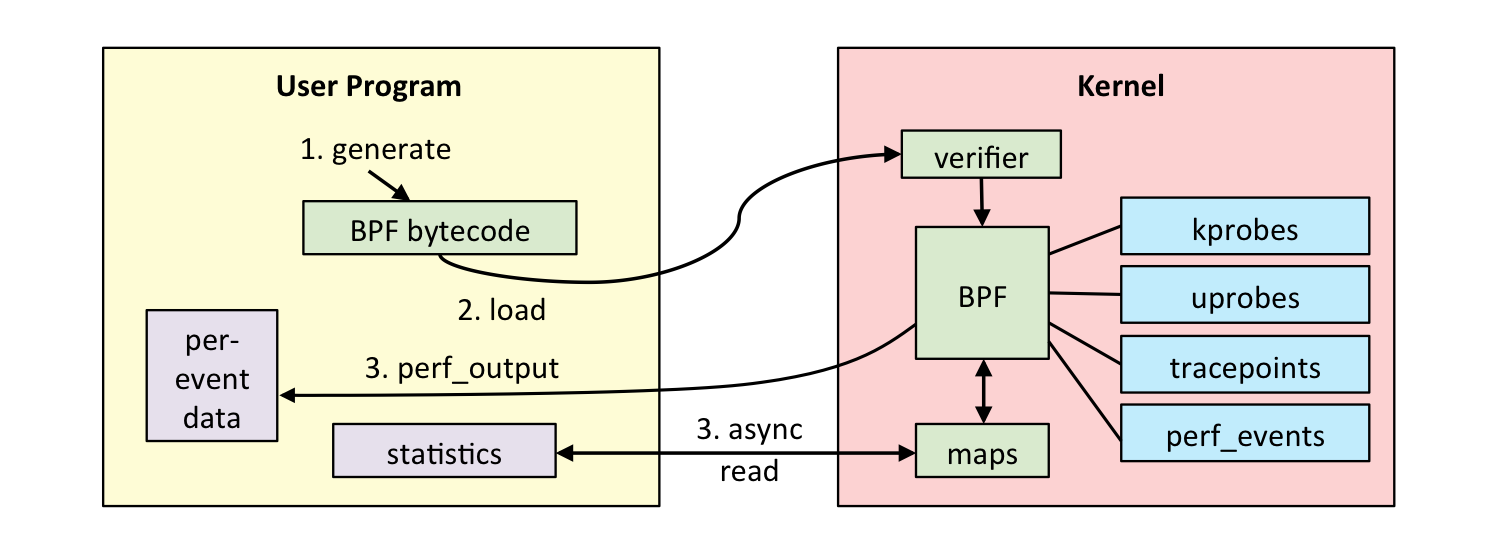
\includegraphics[scale=0.3]{images/linux_ebpf_internals}
  \caption{Detalle de cómo funciona un programa \emph{eBPF} y su relación con el \emph{kernel}. \emph{Autor: Brendan Gregg}}
  \label{fig:ebpf-internals}
\end{figure}

El proyecto \emph{bcc} incluye pequeñas utilidades que sirven para monitorizar algunas partes del sistema. En la figura \ref{fig:bcc-tracing-tools}, puede observarse un diagrama que incluye algunas de ellas
con referencia al sistema que monitorizan.

\begin{figure}[h]
  \centering
    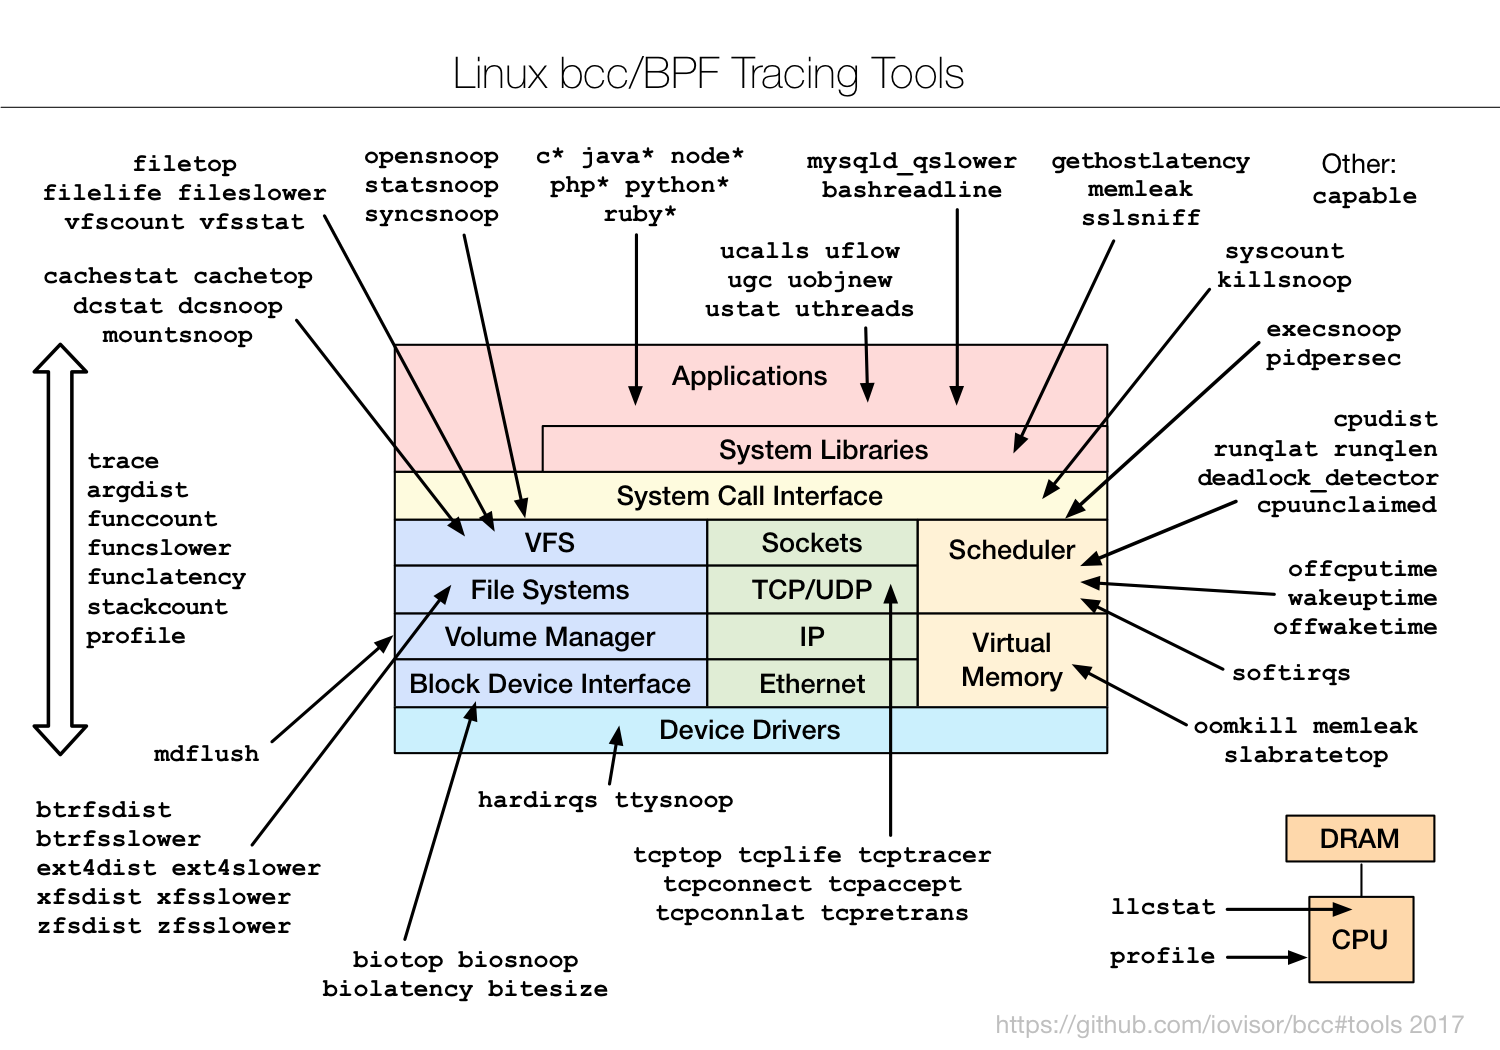
\includegraphics[scale=0.65]{images/bcc_tracing_tools}
  \caption{Relación de utilidades \emph{bcc} y subsistemas monitorizados. \emph{Autor: Brendan Gregg \& iovisor project}}
  \label{fig:bcc-tracing-tools}
\end{figure}

\begin{figure}[h]
  \centering
    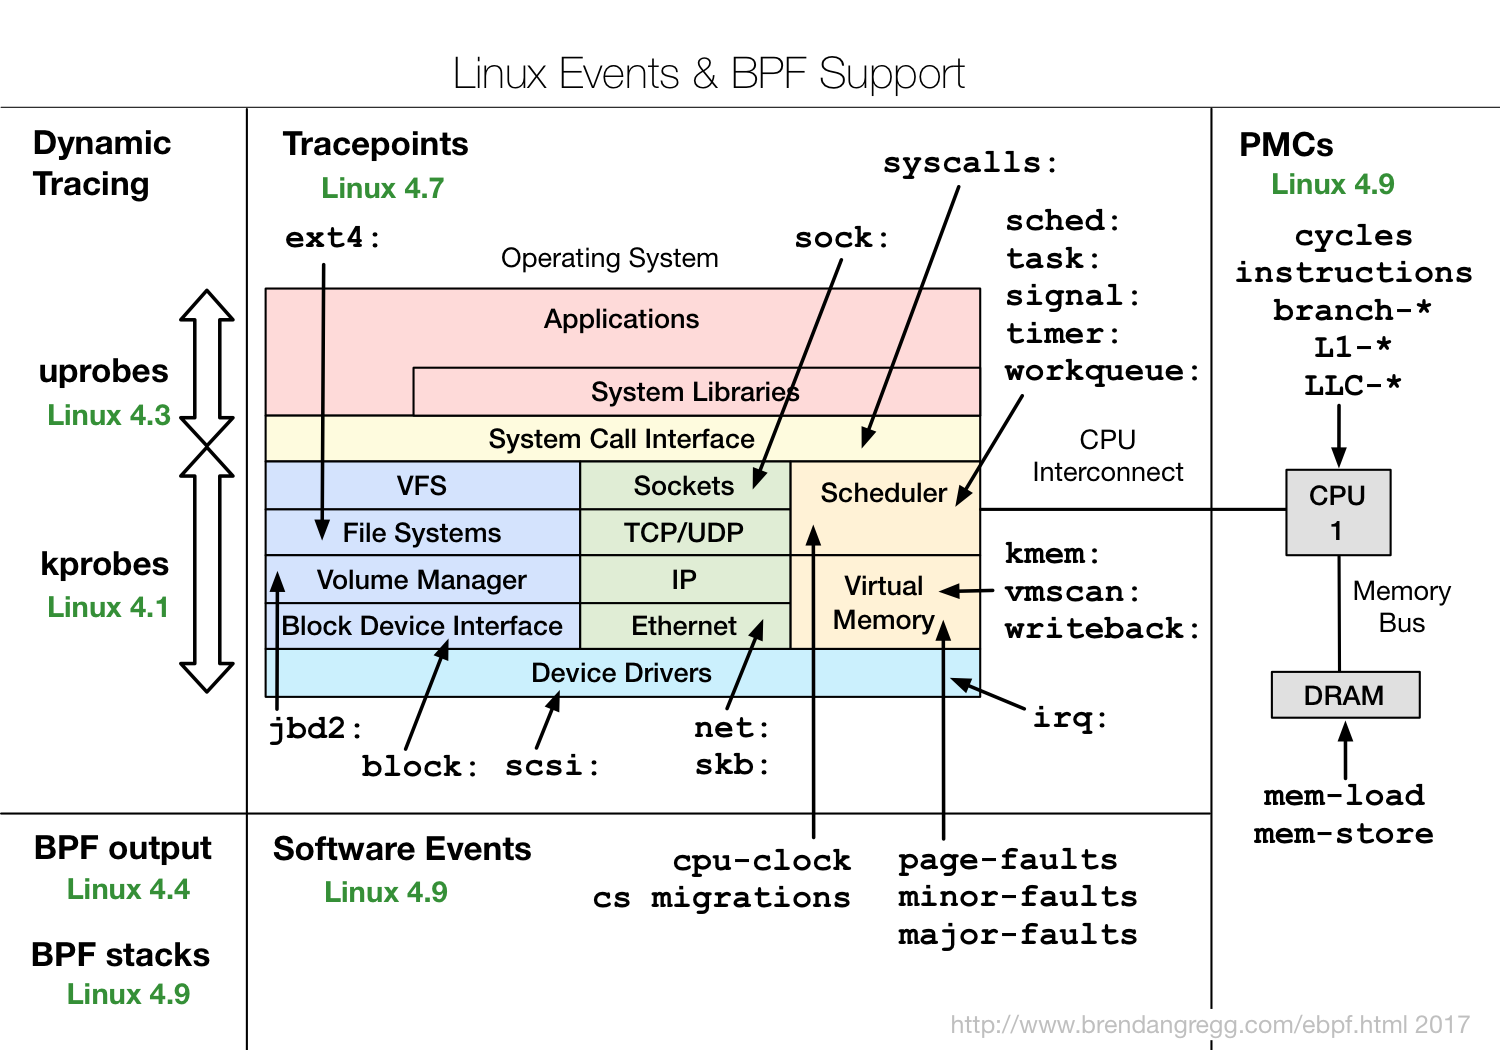
\includegraphics[scale=0.65]{images/linux_ebpf_support}
  \caption{Relación de versiones del \emph{kernel} donde se dan soporte a susbsistemas en \emph{eBPF}. \emph{Autor: Brendan Gregg \& iovisor project}}
  \label{fig:linux_ebpf_support}
\end{figure}

\begin{table}[h]
\centering
\begin{tabular}[!h]{|l|}
\hline
Linux 4.12 Released 2 July, 2017 \\
\hline
Linux 4.11 Released 30 April, 2017 \\
\hline
Linux 4.10 Released 19 February, 2017 \\
\hline
Linux 4.9 Released 11 December, 2016 \\
\hline
Linux 4.8 Released 2 October, 2016 \\
\hline
Linux 4.7 Released 24 July, 2016 \\
\hline
Linux 4.6 Released 15 May, 2016 \\
\hline
Linux 4.5 Released 13 March, 2016 \\
\hline
Linux 4.4 Released 10 January, 2016 \\
\hline
Linux 4.3 Released 1 November, 2015 \\
\hline
Linux 4.2 Released 30 August, 2015 \\
\hline
Linux 4.1 Released 21 June, 2015 \\
\hline
Linux 4.0 Released 12 April, 2015 \\
\hline
\end{tabular}
\caption{\label{tab:linux-release-date}Fecha de publicación de versiones de Linux \emph{4.X}}
\end{table}

Sin embargo, el soporte a subsistemas ha sido introducido de manera paulatina, desde la introducción de \emph{eBPF}. Como referencia, véase el cuadro \ref{tab:linux-release-date} donde se incluye la fecha de publicación de algunas versiones de la rama
\emph{4.x} y la figura \ref{fig:linux_ebpf_support}, donde se aprecia en qué versión del \emph{kernel} se incluye.

\clearpage


Si se utiliza \emph{eBPF}, se encuentran diferencias notables respecto a otras opciones. Las diferentes ventajas e incovenientes más importantes con respecto a \emph{Auditd} y otras opciones son:
\begin{enumerate}
    \item \textbf{Eficiencia}: el procesado de eventos y filtrado se hace dentro del \emph{kernel} en un entorno aislado, lo que es mucho más
    rápido y menos costoso que copiar el evento a espacio de usuario y filtrarlo allí.
    \item \textbf{Prometedor}: aunque \emph{eBPF} es de incorporación reciente, utiliza una tecnología existente en el \emph{kernel} desde hace más de 20 años.
    \item \textbf{Falta de soporte}: no se puede olvidar que lo que se persigue es instrumentar una \emph{honeypot} y que aunque es viable escribir aplicaciones \emph{eBPF} capaces de instrumentar, no hay demasiada documentación al respecto
    y quizá ese objetivo sea merecedor de un proyecto por sí solo.
    \item \textbf{Soporte reciente}: si se pretende utilizar todas las capacidades de \emph{eBPF} es necesario, al menos, un \emph{kernel 4.10} que no está disponible aún en todas las distribuciones y que suelen instalar en
    versiones \emph{LTS} (4.4 actualmente), no estando disponible en la mayoría de proveedores de servidores como \emph{AWS, Digital Ocean \ldots}. Aunque no es imposible instalar nuevas versiones del \emph{kernel},
    supone un esfuerzo extra y un coste para el proyecto.
\end{enumerate}

Por estas razones se descarta el uso de \emph{eBPF} que, aun siendo prometedor, todavía no es suficientemente estable para acometer este proyecto.

\subsection{Obtención de la información del \emph{kernel}: crear un módulo}
\label{subsec:kernel-modulo}

Dado que por las razones expuestas anteriormente, extraer información vía interfaces externas no parece factible, hay que explorar otras opciones.
El \emph{kernel} de \emph{Linux} es modular y, por tanto, se le puede inyectar un módulo de código que extienda las capacidades del \emph{kernel} kernel; esta es, por ejemplo, la manera
en que habitualmente se cargan nuevos controladores.

Ya que extraer información a través de interfaces conocidas no es una opción válida, queda la posibilidad de crear una propia. 
Desarrollar un módulo del \emph{kernel} para generar eventos y procesarlos no es una tarea sencilla ya que el módulo debe ser eficiente y correcto. ``Eficiente'' para procesar el volumen
de eventos y ``correcto'' para no provocar un fallo en el \emph{kernel} que deje inutilizado el sistema.

El esfuerzo y tiempo de dedicación necesarios para crear un módulo de \emph{kernel} con cierta calidad y características necesitaría de una gran inversión de tiempo de desarrollo; quizás de la talla
de este mismo proyecto. Por ello, antes de comenzar esa tarea cabe buscar si hay opciones disponibles que eviten ese trabajo extra.

\emph{Sysdig} (\cite{sysdig-project}) es un proyecto de \emph{Draios} que consta de una \emph{CLI (Command Line Interface)} que utiliza eventos de un módulo del \emph{kernel}
licenciado con GPLv2, lo que supone un encaje perfecto para las necesidades del proyecto.

Ventajas e inconvenientes de este enfoque son:

\begin{enumerate}
    \item \textbf{Coste}:\emph{sysding} obtiene los eventos en el espacio del \emph{kernel} pero los copia a espacio de usuario para ser
    filtrados y procesados. Si el filtro que escogemos es suficientemente amplio se necesitará una importante cantidad de recursos de CPU y de memoria para el filtrado y procesado de eventos.
    \item \textbf{Flexibilidad}:\emph{sysdig} como cliente del módulo del \emph{kernel}, proporciona una enorme flexibilidad a la hora de definir filtros y varios formatos de salida (JSON, formato variable \emph{a la printf},\ldots).
    \item \textbf{Almacenaje}:\emph{sysdig} guarda a disco las trazas en fichero en un formato binario propio que es posible leer y filtrar con posterioridad. Proporciona además opciones para el rotado automático por tamaño y/o fecha,
    lo que permite el almacenaje y gestión de ficheros de trazas directamente desde \emph{sysdig} y la capacidad de reprocesar eventos si los filtros originales son generalistas. 
\end{enumerate}

Las ventajas superan los incovenientes en este caso, ya que aunque el consumo de CPU sea más elevado, poder gestionar las trazas directamente, reprocesar ficheros de captura y tener flexibilidad en las opciones de filtrado y postprocesado hacen de esta opción la finalmente escogida.

\subsection{Notificación de alertas en base a eventos capturados en las trazas}
\label{subsec:alertas-trazas}

Una vez establecido cómo obtener los eventos, el siguiente paso es cumplir con la necesidad de que -en ciertas condiciones- algún componente (ya sea el método de instrumentación o un sistema externo) notifique cuando se vulnera nuestra \emph{honeypot} o hay un
cambio relevante dentro de ella.

Esta notificación es necesaria para conocer cuándo se produce un incidente y, sobre todo, para tener la capacidad de limpiar el entorno tras una
cierta ventana de tiempo de exposición ya que nuestro objetivo es el de aprender de nuestros atacantes y no el de convertirnos en una plataforma de soporte
para ellos.

Desgraciadamente, al comienzo de este proyecto (Marzo de 2016) no existía ningún tipo de aplicación que realizase esta tarea.
Por ello, extender \emph{sysdig} para realizarla pareció lo más apropiado. La manera de extension puede ser a través de un
\emph{script en Lua} que sea ejecutado dentro de \emph{sysdig} o procesando la salida en una aplicación externa.

\emph{Lua} es un lenguaje pequeño, versátil, potente y -posiblemente- capaz de realizar esta tarea, pero la poca familiaridad del autor con este lenguaje decanta
la balanza a favor de desarrollar una aplicación externa que, recibiendo los eventos procesados por \emph{sysdig}, genere las notificaciones.

Afortunadamente (o desgraciadamente por el tiempo ``invertido''), antes de que el desarrollo de dicha aplicación terminase, \emph{Draios} lanzó \emph{Falco} (\cite{falco-project}) en Mayo de 2016; un proyecto cuyo objetivo
es el de analizar el comportamiento anómalo de \emph{containers} en base a filtros de \emph{sysdig} y generar notificaciones sobre ello.

El encaje con los propósitos del proyecto es perfecto y, por ello, se descartó el desarrollo propio tras una prueba inicial.

\subsection{Modelo de riesgo de la sonda y del servicio expuesto.}
\label{subsec:riesgos}

El objetivo de una  \emph{honeypot} es el de engañar a atacantes para que realicen un ataque como lo harían en un entorno real. Aunque este ataque se produce en un entorno en el que dicho ataque es "esperado", se ha de definir el riesgo asumido al exponerse y qué medidas o políticas se aplicarán para estos riesgos. En la figura \ref{fig:riesgo_sonda} están descritos, realizando un diagrama de riesgos siguiendo la metodología expuesta en \cite{Shostack:2014:TMD:2829295}.

\begin{figure}[!h]
  \centering
    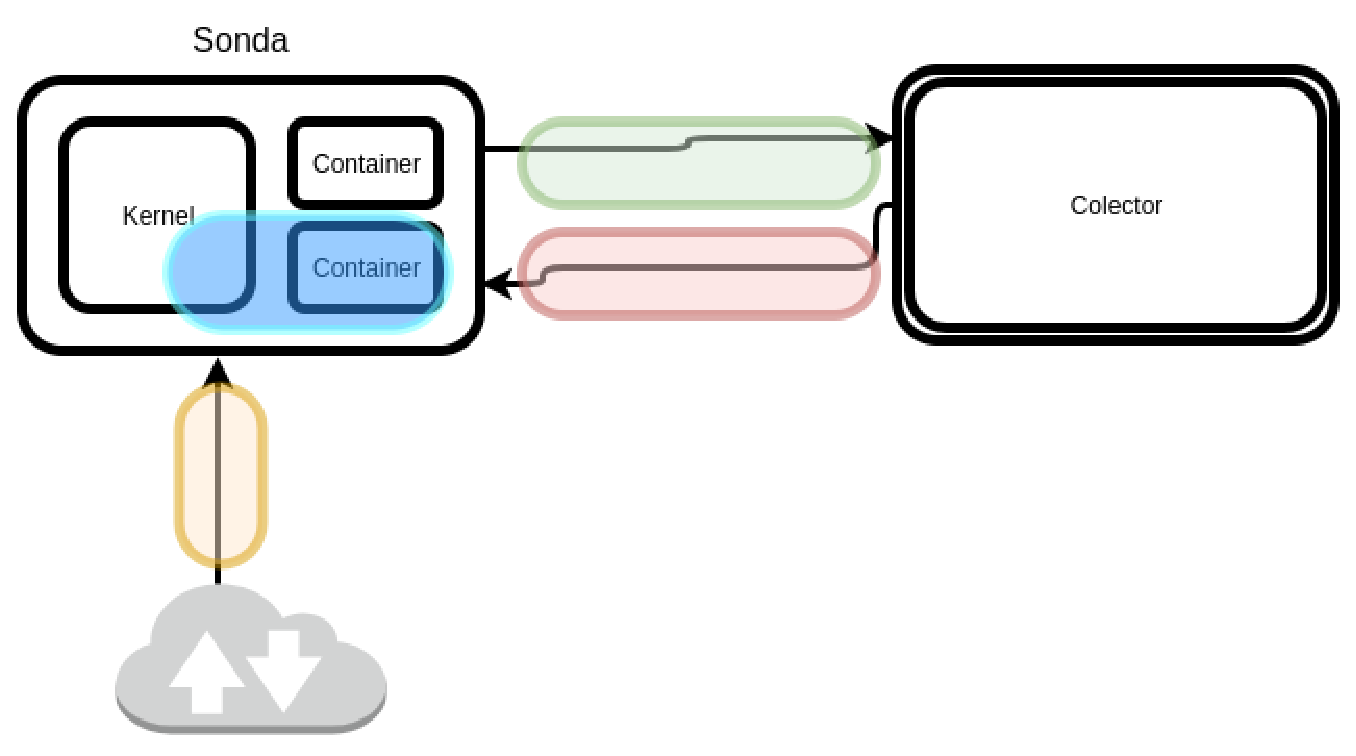
\includegraphics[scale=0.4]{images/threat_model_probe}
  \caption{Modelo de riesgo de la sonda}
  \label{fig:riesgo_sonda}
\end{figure}

Listado de riesgos analizados sobre la figura \ref{fig:riesgo_sonda}:
\begin{enumerate}
    \item \emph{Naranja 1}: elevación de privilegios atacando a un servicio expuesto que no pertenece a la \emph{honeypot}. Un atacante puede explotar un servicio de soporte como un servidor SSH de administración o un servicio interno expuesto por mala configuración.
    \item \emph{Naranja 2}: riesgo de que la \emph{honeypot} sea reconocible o listada. La \emph{honeypot} es conocida por alguna característica (\emph{IP del servidor, versión del servicio,\ldots}) marcándola como \emph{honeypot} y permitiendo a los atacantes simplemente ignorarla.
    \item \emph{Azul}: el atacante escapa desde el \emph{container}. Hay una elevación de privilegios que rompe el aislamiento del \emph{kernel} y el atacante gana acceso a otros \emph{containers} o al servidor.
    \item \emph{Verde}: \emph{spoofing} de la información enviada al recolector. Una vez el atacante gana acceso al servidor, puede enviar al recolector la información falseada.
    \item \emph{Rojo}: elevación de privilegios de un atacante que ya ha conseguido acceso al recolector. El recolector y la sonda mantendrán una conexión y, si alguien ataca al recolector y gana privilegios, puede atacar a las sondas. Pese a que es un riesgo, si el recolector ha sido vulnerado, que ataquen las sondas no es tan grave.
\end{enumerate}

Listado de mitigaciones para los riesgos analizados:
\begin{enumerate}
    \item \emph{Naranja 1}: reducción de la superficie de ataque, eliminación de los servicios expuestos que no pertenezcan a la \emph{honeypot} o limitación del acceso a ciertas direcciones \emph{ip} conocidas.
    \item \emph{Naranja 2}: para mitigar este riesgo, las versiones de las aplicaciones expuestas deben estar ocultas o ser indistinguibles. La mejor alternativa para mitigarlo es reciclar las sondas y crear sondas nuevas con suficiente frecuencia. Si el sistema de provisionamiento y configuración de sondas es automático, se pueden crear nuevas sondas con frecuencia diaria u horaria.
    \item \emph{Azul}: aceptación del riesgo que supone que el \emph{container} siempre tendrá acceso al \emph{kernel} que se comparte con otros \emph{containers} y el servidor. Como mitigación, podemos restringir los privilegios del \emph{container} para que solo pueda utilizar algunas \emph{syscalls} pero -en cualquier caso- el riesgo de compromiso de un servidor a través de un \emph{container} siempre estará presente. 
    \item \emph{Verde}: la comunicacion entre sonda y recolector se realizará a través de un canal cifrado con clave asimétrica. En el lado del recolector se pueden realizar validaciones de entrada antes de guardar en base de datos o actuar sobre los eventos recibidos.
    \item \emph{Rojo}: de todos los riesgos listados, este es el menos grave. Si el recolector ha sido atacado y vulnerado, tendremos problemas mayores que nuestra sonda sea atacada. La mitigación en este caso es si se ha vulnerado: cerrar el entorno, apagar los servidores, guardar periódicamente la información obtenida en un almacenamiento diferente y externo, hacer una auditoria de seguridad y realizar el análisis de qué provocó el ataque para repararlo y recrear el entorno desde cero para tener la seguridad de que el atacante no tiene acceso a él.
\end{enumerate}

Tendremos que tener en cuenta estos riesgos a la hora de modelar la arquitectura y diseñar las protecciones, en general los riesgos \emph{Naranja 1}, \emph{Naranja 2} y \emph{Azul} son mas prioritarios que los riesgos \emph{Verde} y \emph{Rojo}. Las posibles acciones a tomar estan listadas en las mitigaciones del mismo color y creemos que son suficientes para equilibrar los riesgos.

\section{Análisis de soluciones para el recolector}


\subsection{Registro de las sondas}

El recolector debe conocer el número de sondas desplegadas para poder extraer información de ellas o, al menos, validar
los eventos que estas envíen.

En definitiva, las preguntas a resolver son: ¿cómo se realizará el registro de sondas? y ¿qué casos de uso ha de proporcionar? En general, es necesario lo siguiente:

\begin{enumerate}
    \item La \emph{metadata} de las sondas para la explotación de datos, al menos la ubicación donde la sonda está desplegada, el proveedor y servicios expuestos en la \emph{honeypot} y en sus versiones.
    \item Como se comentaba en el modelo de seguridad de las sondas, estas son consideradas entidades efímeras, que aparecen y desaparecen. 
    Así, también es necesario un registro de sondas para realizar los análisis históricos, especialmente, si se quiere permitir el reprocesado de datos.
    \item La verificación de la sonda para mantener la integridad de la información. La sonda ha de identificarse frente al recolector para tener la seguridad de que la fuente de información es legítima.
    \item De cara a la recolección de datos, la elección de un modelo \emph{pull} frente a uno \emph{push}. En caso de escoger un modelo \emph{pull}, el recolector debe conocer
    cuales son las sondas y su estado para obtener las trazas.
\end{enumerate}

\subsection{Recolecci\'on de notificaciones de la \emph{honeypot}}

Las alertas generadas por la \emph{honeypot} serán eventos en formato textual o binario de un tamaño pequeño ( $<$ 1MiB). 
Es importante que dichos eventos no se pierdan y que sean recolectados con la mayor celeridad posible incluso si las trazas disponibles
y la información de las trazas no está disponible.

Para la recolección de estas notificaciones, hay las opciones que se listan a continuación.

\subsubsection{Notificaciones a través de HTTP}

Cuando detecta un evento relevante, la \emph{honeypot} realiza una petición HTTP a un servicio web de recolección que se ejecuta en el recolector.
Si dicho servicio no está disponible o está congestionado, el evento se perderá.
La sonda no requiere instalación adicional de \emph{software} ya que solo requiere realizar una petición HTTP. 
Si la conexión de red de la sonda no funciona al realizar la petición, el evento también se perderá.

\subsubsection{Notificaciones usando un sistema de colas}
\label{subsec:notificaciones-falco}


Habrá que instalar, configurar y mantener un sistema de colas como \emph{RabbitMQ, ZeroMQ, Kafka} 
o pagar por el uso de sistemas de colas en el \emph{cloud} como \emph{AWS SQS, AWS Kinesis o Google Cloud PubSub}.

La principal ventaja al seguir este enfoque es que los eventos serán almacenados en el sistema de colas y no en las sondas o en el recolector. Si queremos
distribuir las tareas de procesamiento y recolección de eventos entre varios recolectores, este elemento central de coordinación es un requisito imprescindible.

El principal inconveniente es el coste en términos económicos y de esfuerzo en mantener esta solución. 
Si decidimos gestionarlo dentro del proyecto usando algo como \emph{RabbitMQ o Kafka} además del incremento económico en servidores 
se le debe añadir el incremento en la complejidad del proyecto. En cambio, si se apuesta por utilizar una solución \emph{cloud}, la complejidad
de instalación y mantenimiento baja a costa de un mayor desembolso económico y de aceptar las capacidades técnicas y límites que las soluciones 
\emph{cloud} tienen.

Para este proyecto, el orden estricto de recepción de eventos no es necesario. De modo que no importará el orden de eventos recibidos siempre y cuando
ningún evento se entregue con demasiada posterioridad.
\begin{table}[h]
    \centering
    \begin{tabular}[!h]{|l|l|r|}
    \hline
    \thead{Opcion} & \thead{Comentarios} & \thead{Coste aproximado} \\
    \hline
    \emph{AWS SQS} & 10.000.000 de peticiones, 3 GiB de transferencia & 5\$ mes \\
    \hline
    \emph{Google PubSub } &  10 GiB de eventos & 0.36\$ mes \\
    \hline
    \emph{RabbitMQ} & 3 instancias (512 MiB,1 CPU, 20 GiB de disco) & 15\$ mes \\
    \hline
    \end{tabular}
    \caption{\label{tab:colas-coste} Coste aproximado mínimo de sistemas de colas}
    \end{table}


El cuadro \ref{tab:colas-coste} refleja el coste de sistemas actuales con el precio fijado en la fecha de redacción de esta memoria. En él no se contemplan costes indirectos,
como el coste de las horas invertidas en configurar la puesta a punto del sistema, que en el caso de las soluciones \emph{cloud} aun no siendo cero, es menor que la solución de hacerlo \emph{in-house}.

Tampoco se tiene en cuenta la escalabilidad de la solución; que en el caso de las soluciones \emph{cloud}, el sistema es escalable a costa de un precio cada vez mayor, mientras que en la solución \emph{in-house}, los costes son
fijos hasta que se consuma toda la capacidad. El volumen de eventos a procesar dependerá de las condiciones de red de la instalación y el volumen de eventos por lo que no es posible
proporcionar un número de referencia de eventos a procesar ``a priori''.

Las soluciones \emph{cloud} tienen un coste indirecto y ligan a un proveedor en concreto. Si se escoge que nuestras \emph{honeypots} se desplieguen en otros proveedores diferentes, se han de hacer
pruebas de red para saber si la conectividad entre proveedores es buena, y tendrá costes adicionales en términos de tráfico de red.

Los proveedores de servicios de computación en exclusiva (como \emph{VPS}, \emph{Housing}) no suelen cobrar el tráfico de red a no ser que se superen ciertos umbrales.

\subsubsection{Notificaciones usando un recolector de \emph{logs}}
\label{subsubsec:usando-rsyslog}

Esta opción se puede considerar como un híbrido de las anteriores, en tanto que es la instalación de una aplicación de recolector de \emph{logs} en la sonda. 
La sonda escribirá eventos en disco cuando estos se produzcan, el sistema de recolección de \emph{logs} los monitorizará en disco y
se encargará de reenviar estos eventos al recolector, preferentemente, utilizando un canal seguro para la transmisión.

Si hay problemas en la conectividad de red entre la sonda y el recolector, los eventos se guardarán en un \emph{buffer} en disco y se reenviarán cuando la parte servidor esté disponible.

Como ejemplo de estas aplicaciones de recolección de \emph{logs} podemos citar a \emph{rsyslog,logstash,syslog-ng o fluentd}. \emph{Rsyslog} y \emph{syslog-ng} son más veteranas y \emph{logstash} y \emph{fluentd}, más recientes. 

La diferencia entre las antiguas y recientes radica en que las recientes hacen énfasis en la capacidad de manipulación de los \emph{logs} antes de su envío, mientras
que las antiguas están más probadas y su enfoque garantiza el envío de \emph{logs} de manera segura.

El coste computacional de estas soluciones (aunque no es negligible) es muy bajo y es necesario procesar un volumen muy elevado de \emph{logs} para que tenga impacto.
El recolector deberá encargarse de ser capaz de albergar todos los \emph{logs} recibidos, ya sea porque a su vez reenvía los \emph{logs} a otra ubicación o porque se encarga de la 
política de rotado. 

\subsubsection{Opción escogida}

Para este proyecto, ha sido escogida la opción de utilizar un recolector de \emph{logs} en nuestras sondas y para que los reenvíe a nuestro recolector de eventos. 

\begin{enumerate}
    \item La opción de notificar mediante peticiones HTTP es la más simple desde el punto de vista de la sonda y la más deseable, pero no otorga garantías de entrega.
    \item El uso de sistemas de colas es lo deseable para escalar la solución ya que desacopla los productores de eventos de los consumidores,
     y, para la sonda, la semántica de entrega es igual de simple que en el caso de la opción HTTP. Sin embargo, el coste económico y la complejidad elevada que introduce no justifica su acogida.
     En un estado posterior del proyecto, siempre se puede pivotar a utilizar un sistema de colas.
\end{enumerate}

En concreto, se utilizará \emph{rsyslog} como recolector de \emph{logs} por su poca necesidad de memoria y CPU y por su estabilidad. Las capacidades de modificación de \emph{logs}
antes de su envío no son necesarias para este proyecto y \emph{logstash} y \emph{fluentd} tienen un \emph{footprint} de uso de memoria mucho más elevado.

\subsection{Recolección de trazas}

Las trazas generadas por la \emph{honeypot} serán ficheros binarios de un tamaño elevado ($>$ 25 MiB). En él se recogerán todos los eventos del sistema instrumentalizado (\emph{syscalls}, datos,\ldots).
Se deberá buscar un sistema que permita recolectar todas las trazas de todas las sondas. Es importante notar que
las trazas una vez procesadas no son estrictamente necesarias, aunque es útil mantener un histórico de ellas por dos motivos:

\begin{enumerate}
    \item Permitir el estudio analítico en base a un histórico.
    \item Facilitar el reprocesamiento en caso de errores de procesado (\emph{backfilling}). Idealmente, este método de extracción de
    datos debería ser correcto y tener los suficientes tests y garantías, pero aún así los errores pueden ocurrir.
\end{enumerate}

\subsubsection{Envío de trazas a almacenamiento en la nube}

Si se decidiera no gestionar las trazas nosotros, se podría optar por almacenar las trazas en la nube en soluciones \emph{cloud}. Para conocer el coste aproximado, se hará con el supuesto de que el almacenaje será de 500GiB de trazas por mes (aprox 18 GiB por día). En ese caso, el coste en \emph{AWS} y \emph{Google Cloud} para almacenarlos
en una región europea, teniendo en cuenta los costes de tráfico de salida fuera del proveedor sería:

\begin{table}[h]
    \centering
    \begin{tabular}[!h]{|c|c|}
    \hline
    \thead{Proveedor} & \thead{Coste en dolares} \\
    \hline
    \emph{AWS}, resto de servidores fuera &  57.52 \$ \\
    \hline
    \emph{Google Cloud}, resto de servidores fuera &  78.08 \$ \\
    \hline
    \emph{AWS}, con servidores en mismo proveedor  &  11.89 \$ \\
    \hline
    \emph{Google Cloud}, con servidores en mismo proveedor & 10.44 \$ \\
    \hline
    \end{tabular}
    \caption{\label{tab:almacenamiento-coste} Coste aproximado de almacenamiento en la nube para 500 GiB}
    \end{table}

En el cuadro \ref{tab:almacenamiento-coste} se reflejan los costes mensuales de almacenar 500 GiB. 

Aunque eso obliga a comprar servidores en el mismo proveedor que puede elevar el coste total del proyecto, en él se observa que es sensiblemente más barato si no hay transferencia de datos fuera del proveedor.

\subsubsection{Sistema de archivos distribuido}

Otra opción se basa en montar un sistema de archivos distribuido dentro del proyecto y no usar sistemas de almacenamiento externos
en la nube. Como ventajas:

\begin{enumerate}
    \item El sistema de archivos es infinito e ilimitado en espacio para la aplicación.
    \item La interfaz de comunicación puede ser como un punto de montaje más en el sistema de archivos o a través de 
    peticiones HTTP a la \emph{S3}.
    \item El rotado, eliminación, mantenimiento y ajuste de los archivos dentro del sistema de archivos es responsabilidad de este mismo.
\end{enumerate}

En cambio, como inconvenientes, hay:

% se necesita una buena conexion de red.
% punto critico si cae
% sistemas complejos no faciles de mantener

\begin{enumerate}
    \item La necesidad una buena conexión de red entre los servidores que conformaran el sistema de archivos distribuido y entre estos y las sondas y el recolector como clientes. 
    Por la naturaleza del proyecto, interesa tener las sondas en diferentes proveedores y diferentes regiones. La conectividad entre diferentes proveedores y regiones es muy irregular, por lo que se podría contar con una conexión de red estable y/o rápida.
    \item El peligro de que el sistema de archivos distribuido se convierta en un punto crítico (\emph{SPOF, Single Point of Failure}). A pesar de intentar que el sistema de archivos sea distribuido y escalable en caso de error del sistema, el sistema dejará de funcionar en su totalidad.
    Las sondas dejarán de ser capaces de publicar las trazas en el sistema de archivos, y los procesadores de datos serán incapaces de leer nuevas trazas y procesarlas.
    \item La complejidad de optimizar, configurar y mantener estos sistemas y que requieren una inversión inicial y sostenida de esfuerzo para ser operados.
\end{enumerate}

Tradicionalmente, se ha utilizado \emph{NFS} para configurar y utilizar sistemas de archivos en red (no distribuidos) en Linux (véase \cite{wiki-nfs}). 
En el caso de existir la posibilidad de ofertar a potenciales clientes nuestro sistema de archivos como un punto de montaje extra en el sistema, se deberá utilizar
\emph{NFS}, \emph{GlusterFS} (\cite{wiki-glusterfs}) y/o \emph{Ceph} \cite{wiki-ceph}.

La diferencia fundamental del primero con los segundos es que el conjunto de discos duros y almacenamiento en \emph{NFS} está gestionado de manera local
por cada nodo que forme parte del sistema, en tanto en cuanto en sistemas como \emph{GlusterFS} y \emph{Ceph} los nodos forman parte de un 
mismo \emph{pool} de discos duros donde se pueden configurar opciones de replicación para garantizar que los archivos no se pierden, en el caso de perder la conectividad a un nodo.

\emph{Ceph} y otros poyectos como \emph{\href{https://minio.io/}{Minio}} proveen de una interfaz compatible con \emph{AWS S3}, que puede ser una ventaja importante
si se pretende migrar de un sistema a otro y que, ademas, simplifica la configuración en los clientes.

En lugar de tener que montar el sistema de archivos como cliente de nuestro sistema de archivos distribuido basta 
realizar peticiones HTTP a un servidor. De esta manera la configuración del sistema es menor y mucho más simple.

\subsubsection{Envío de trazas a un servidor interno de almacenamiento}.

Otra opción será utilizar el almacenamiento local en las sondas y el almacenamiento local en el recolector para guardar las trazas.
Las sondas escriben las trazas en el disco local y,a su vez, algún proceso en el recolector se encarga periódicamente de conectarse a las sondas,
comprobar si hay nuevas trazas y descargarlas.

Las ventajas de este enfoque son:
\begin{enumerate}
    \item La no incursión en costes adicional por utilizar el almacenamiento local.
    \item La estabilidad de la red deja de ser un problema. Si la red no está disponible o es lenta, entre las sondas y el recolector se irán almacenando las trazas mientras haya espacio.
    \item La facilidad para combinar con uno de los dos enfoques anteriores para almacenamiento de carácter más permanente.
\end{enumerate}

Por otro lado, presenta los siguientes inconvenientes:

\begin{enumerate}
    \item La latencia de entrega de trazas puede ser mayor y en cualquier caso es variable.
    \item La posibilidad de perder trazas debido a pérdidas de conexión de red entre la sonda y el recolector son muy prolongadas.
    \item El almacenamiento es finito y no fácilmente ampliable, lo que implica que se han de eliminar trazas para asegurar que las trazas nuevas puedan
    ser procesadas.
\end{enumerate}

Para implementar este enfoque se necesita una herramienta para la transmisión eficiente y sincronizada de archivos. Para este fin,
\emph{rsync} es una herramienta clásica ampliamente utilizada (citada por ejemplo en \cite{Ph.D.200301} y \cite{douglis2004web}). Y deberá limitar el ancho de banda que \emph{rsync} utilizará para evitar la congestión de la red para otros usos.
% rsyslog 

\subsubsection{Opción escogida}

La opción escogida será la tercera. Siempre se puede cambiar e incorporar una de las otras opciones más adelante, cuando el proyecto lo requiera y el gasto económico
y/o la complejidad añadida supere con mucho las ventajas que aportan.

Enviar trazas a través de \emph{rsync} tiene sus propios retos. Se acepta pues, que se podrán perder trazas y que no se almacenarán
demasiadas trazas para el análisis histórico y/o para poder reprocesar.

A pesar de lo anterior, su simplicidad y bajo coste -junto a su compatibilidad con otras opciones- la convierten en la opción escogida.

\subsection{Modelo de datos del sistema}
\label{subsec:modelo-de-datos}

No se entrará en el detalle de qué sistema de gestión de bases de datos será utilizado, pero sí  se ha de analizar cual es el modelo de datos
adecuado para el proyecto en el contexto del dominio.

La información extraída es muy relevante cuando es reciente y pierde relevancia en muy poco tiempo. Es decir, la información de un ataque realizado
hace un año es poco relevante porque habrán surgido nuevas versiones del \emph{software}, porque el método de ataque ya habrá sido analizado y porque el único interés
que tiene es como aportación para un estudio estadístico.

Por ello, nuestro modelo de datos estará modelado como una serie temporal con foco en la búsqueda. La inserción de datos se realizará con poca frecuencia, idealmente una vez,
y, posiblemente, nuestro modelo no sea relacional o no evidentemente relacional, ya que la integridad de los datos no es tan relevante.
En el caso de tener una alerta sin más información adicional (aunque no tiene tanto valor como una alerta con toda la información) ya será de por sí relevante.

\section{Análisis de soluciones para la explotación}

\subsection{Generalidades}

De cara a la explotación de datos, debemos presentar a los potenciales usuarios de una interfaz. Esta interfaz puede estar
orientada a humanos o a aplicaciones. Es evidente que, en algún momento, hay que representar visualmente la información para que algún usuario pueda explotarla.
La cuestión es sí debemos enfocar el esfuerzo del proyecto a crear esta visualización o merece más la pena construir
una interfaz para aplicaciones y dejar a terceros la construcción de visualizaciones finales.

\begin{enumerate}
    \item \textbf{Informes}: incluyen habitualmente gráficas-resumen y datos de carácter estadístico y son útiles para reconocer tendencias y patrones, pero no lo son para actuar frente un ataque en tiempo real.
    \item \textbf{API}: una interfaz para aplicaciones que los clientes pueden integrar para responder ante incidentes o construir un informe de manera programática.
\end{enumerate}

Hay diversos ejemplos de \emph{Honeypots} que generan informes como método de explotación del usuario (enlace a un \href{http://www.nothink.org/honeypot_ssh.php}{ejemplo}, también disponible en figura \ref{fig:informe-honeypot}).

\begin{figure}[h]
    \centering
      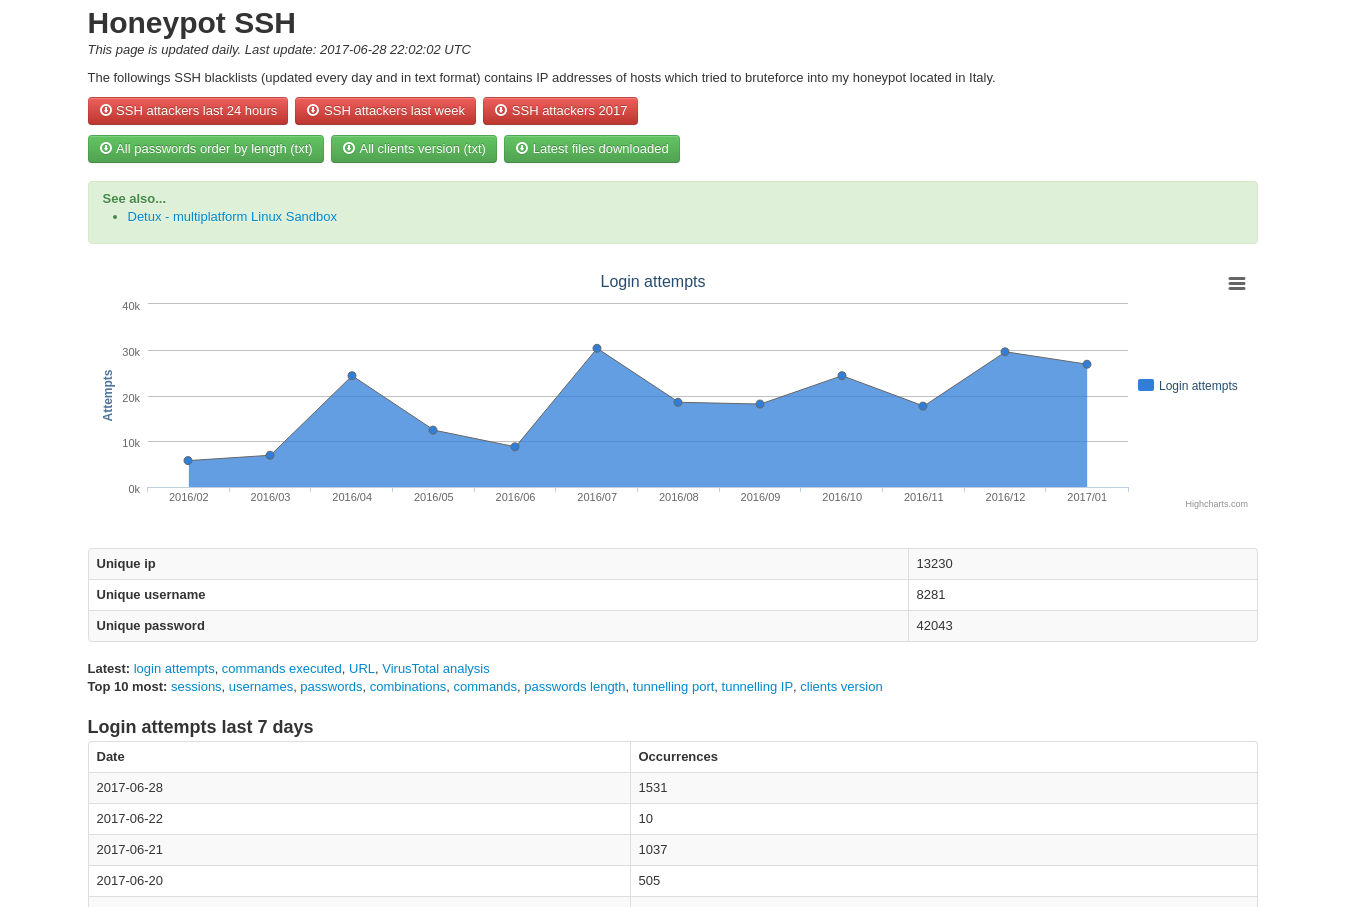
\includegraphics[scale=0.3]{images/honeypot_informe}
    \caption{Ejemplo de informe de \emph{Honeypot}}
    \label{fig:informe-honeypot}
  \end{figure}

El informe es vistoso y permite observar y analizar tendencias y patrones. Pero si queremos responder a un ataque, no es sencillo. Y si, además, estamos interesados en un subconjunto de los ataques,
en un informe no suelen implementarse los filtros necesarios para analizarlos.

Por ello, como herramienta de explotación de datos se ofrecerá una API que terceros puedan utilizar para generar sus informes o procesar los incidentes y responder
en tiempo real.

% 20/08/2017
\subsection{Objeto de la API}

El objeto de la API es la de proveer una interfaz de datos que sea consumible por aplicaciones y que puede ser expuesta en diversos formatos.
Es importante que cuando se describan los actores en un incidente, se haga siempre en referencia a un marco temporal. Los atacantes
en un incidente no tienen porque ser los promotores del ataque. Es más, a menudo, los promotores utilizan máquinas infectadas de sus víctimas para ejecutar el ataque
y, por tanto, sería contraproducente marcar estas víctimas y responder de manera agresiva como puede ser un bloqueo, por ejemplo.

El marco temporal ayuda al cliente a determinar si el atacante es recurrente en sus ataques o víctima, y deja en el cliente la decisión sobre qué realizar al respecto en base a 
las políticas y necesidades de su entorno.

\subsection{API}

La API será de consulta, no se plantea como objetivo la posibilidad de crear incidentes a través de ella. La API será
de tipo \emph{REST} (véase \cite{rest}). Arquitecturar las APIs usando \emph{rest} es un estándar de facto, quizás si nuestra API fuese parte de
un ecosistema complejo y/o que fuese orientado especialmente a móviles, podríamos plantear el uso de \emph{GraphQL} (\cite{graphql}), aunque su madurez
a nivel de herramientas y adaptación no es comparable al de APIS REST.

\subsubsection{Versionado}

La definición del contrato de la API no está basado en experiencia de uso de nuestros clientes, es por ello que tendremos que establecer 
un método que permita la evolución o el cambio de la misma. Existen varios métodos de versionado, entre otros:

\begin{enumerate}
    \item \textbf{Parámetro}: se pasa la versión de la API como parámetro de la petición. Algunos \emph{proxies} pueden eliminar el parámetro y conducir a errores.
    \item \textbf{URL}: la URL contiene la versión de la API a la que se quiere acceder. Su ventaja es que es fácil de saber qué versión se utiliza y es fácil de depurar pero la desventaja es que afea y puede complicar la
    URL.
    \item \textbf{Cabecera HTTP}: se pasa la versión de la API que se quiere usar como una cabecera HTTP. La ventaja es que la URL no cambiará con 
    cada nueva versión de la API. 
\end{enumerate}

Aunque el versionado como cabecera HTTP se adhiera más a \emph{REST}, según algunas fuentes, el versionado por URL es más popular (\cite{3scale-versionado)} y, por ello, escogemos este método.

\subsubsection{Definición de la API}
\label{subsubsec:definicion-api}

\begin{table}[h]
    \centering
    \begin{tabular}[!h]{|c|c|}
    \hline
    \thead{Verbo HTTP} & \thead{URL} \\
    \hline
    GET & /v1/\emph{{aplicacion}}/incidents  \\
    \hline
    GET & /v1/\emph{{aplicacion}}/feed  \\
    \hline
    \end{tabular}
    \caption{\label{tab:definicion-api} Definicion de API externa, de clientes.}
    \end{table}

    Como puede verse en el cuadro \ref{tab:definicion-api}, inicialmente, solo  se le exigen a la API dos funciones: una donde se pidan incidentes y otra, que proporcione un \emph{feed} de intentos de inicio de sesión. 
El modelo concreto que define un incidente y los datos que se han de incluir, dependerá de la aplicación. Puede ser también interesante ofrecer un 
\emph{endpoint} de \emph{feed} que devuelva de manera continua los datos encontrados. La diferencia entre ambos endpoints es que
el de \emph{incidents} devolverá los datos de los incidentes según unos criterios mientras el endpoint de \emph{feed} devolverá 
de manera continua e ininterrumpida los datos que se vayan encontrando.

Para el \emph{endpoint} de incidentes se podrá parametrizar la consulta según los parámetros que pueden verse en el cuadro \ref{tab:parametros-api}. En el caso
de no especificar ninguno, se establecerán por defecto para devolver algún número de eventos recientes.
    \begin{table}[h]
        \centering
        \begin{tabular}[!h]{|l|c|}
        \hline
        \thead{ Nombre} &  \thead{Contenido} \\
        \hline
        from & fecha en formato ISO 8601 \emph{YYYY-MM-DDTHH:MM:SS(Z$|$+-HH:MM)}  \\
        \hline
        to & fecha en formato ISO 8601 \emph{YYYY-MM-DDTHH:MM:SS(Z$|$+-HH:MM)}  \\
        \hline
        size & entero natural positivo \\
        \hline
        \end{tabular}
        \caption{\label{tab:parametros-api} Definición de parámetros la API}
        \end{table}
    
\subsubsection{Formatos de salida}

El objeto de la API es ser utilizada por aplicaciones. Como formato de salida se pueden utilizar \emph{XML} o \emph{JSON}, siendo 
este último más utilizado en la actualidad.

Como esquema de datos, podremos utilizar o basarnos en \emph{STIX} (\cite{oasis-stix}), un lenguaje estructurado para compartir información de seguridad entre organismos
desarrollado por el grupo OASIS.

\chapter{Resultados finales}
\minitoc{}
\section{Arquitectura}

La arquitectura final puede observarse en la figura \ref{fig:arquitectura-general}. En ella se encuentran los siguientes elementos:

\begin{enumerate}
    \item \textbf{Sondas}: desplegadas en varios proveedores y regiones del mundo, serán instaladas y configuradas tantas de ellas como
    diferentes muestras de datos queramos obtener. Es el elemento más dinámico de la arquitectura. El límite del crecimiento lo impone la capacidad
    del recolector y \emph{backend} ya que mientras este sea capaz de absorber y procesar el volumen de datos obtenido en las sondas podremos crear nuevas.
    \item \textbf{PKI y control}: se encarga de las funciones externas como el almacenamiento de secretos (gestiona la \emph{PKI, Public Key Infrastructure,} interna, monitoriza el resto de elementos y lanza el provisionamiento y la configuración.
    \item \textbf{Recolector y \emph{backend}}:se encarga de almacenar las trazas de las sondas y de albergar los servicios encargados para el procesado y la explotación como la API. Este elemento es un \emph{SPOF, Single Point Of Failure,}, si cae el \emph{backend} y la recoleccion quedan inutilizados.
    Las razones para este diseño son puramente económicas y de simplicidad, si queremos un sistema robusto y escalable convendría separar funciones y tener un esquema que permita el escalado horizontal.
\end{enumerate}

\begin{figure}[h]
    \centering
      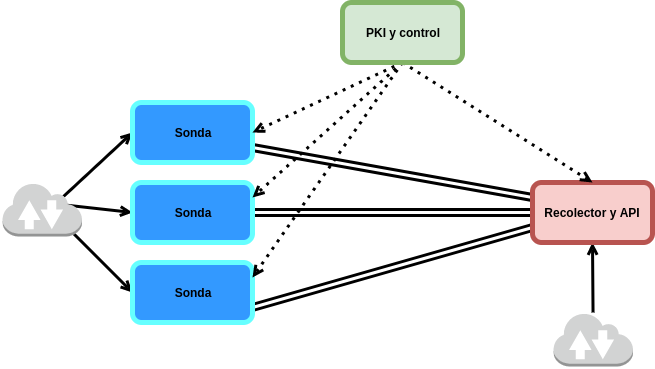
\includegraphics[scale=0.5]{images/arquitectura_general}
    \caption{Diagrama de arquitectura general}
    \label{fig:arquitectura-general}
  \end{figure}

\subsection{Provisión y configuración de servidores}
\label{subsec:server-config}

Uno de las mitigaciones explicadas en \ref{subsec:riesgos} es tener la capacidad de crear sondas con frecuencia. La creación de la sonda implica
los siguientes pasos:

\begin{enumerate}
    \item \textbf{Provisión}: solicitar al proveedor un nuevo servidor de unas características determinadas (o ponerlo en marcha en nuestros \emph{datacenters}).
    \item \textbf{Configuración}: instalación de los paquetes de herramientas, \emph{software} y configuración necesarios para que la sonda pueda funcionar.
    \item \textbf{Operación}: realizar cambios post-configuración tales como la actualización de paquetes de seguridad.
\end{enumerate}

Todos estos pasos pueden ser ejecutados por un operador humano, tal y como a menudo son. Pero si, en nuestro caso, queremos un proceso repetible, rápido y automatizado,
no podemos permitirnos que estos procesos sean manuales ya que imposibilitan crear un nuevo servidor en el orden de minutos.

\subsubsection{Infrastructura como código}
\label{subsec:infra-as-code}

Un enfoque que nos acerca al objetivo de ser capaces de desplegar nuevas máquinas necesarias en un entorno dinámico en minutos, es adoptando la práctica
de infrastructura como código (véase \cite{fowler-infra-as-code}). Dicha práctica se basa en:

\begin{itemize}
    \item Definición en ficheros. Toda la configuración se recoge en ficheros ejecutables, ninguna persona debería entrar en el servidor
    y realizar cambios de configuración manualmente, de hacerlo, estaría creando servidores únicos frágiles (\emph{Snowflake Servers}).
    \item Autodocumentacion. El código documenta el proceso seguido para la configuración sin necesidad de una documentación externa orientada a un humano. Aunque la documentación pueda existir y es aconsejable que en algunos casos exista), esto evita que la documentacion quede anticuada.
    \item Versionado. El código fuente que define la infrastructura se mantiene en un sistema de control de versiones de código, lo que permite ser auditado y lanzar ejecuciones reproducibles (lanzar una versión específica).
    \item Cambios pequeños. Si se realizan cambios pequeños en código es fácil diagnosticar cuando se introducen errores.
\end{itemize}
 
Este enfoque requiere que haya algún proceso de \emph{Continuous Integration} o \emph{Continous Delivery}. De no ser así, la definición de los ficheros
de la configuración no se correspondería con la configuración que se encuentra en los servidores (\emph{Configuration Drift}). Si construímos 
un proceso de aplicación de la configuración que se lance desde algún cambio del código podremos conseguir:

\begin{itemize}
    \item Cambios \emph{in-place}. Se aplicarán los cambios sobre los servidores que ya se ejecuten, cambiando la configuración en caliente de los servicios que corren.
    Se corre el riesgo de dejar el servidor con una configuración incompleta pero, para servidores que manejan datos y/o estado, es normalmente la opción más sencilla. Si la configuración
    está suficientemente probada en un entorno identico al de producción y es correcta los servidores convergerán a la configuración descrita. 
    \item \emph{Phoenix servers}. Cada cambio de configuración involucra crear un servidor de nuevo y configurarlo completamente desde la configuración almacenada.
    Requiere que exista algún mecanismo de promoción entre servidores, así la versión antigua se ejecuta a la vez que la nueva. De otra manera, habría caida del servicio. Los costes pueden ser más elevados que si se sigue una estrategia \emph{in-place}
    puesto que un cambio implica la creación de un nuevo servidor y su configuración completa. Si el proceso de configuración falla a la mitad del proceso, la configuración será inestable y el servidor tendrá un mal funcionamiento.
    \item \emph{Immutable servers}. Es un refinamiento de la estrategia anterior: en lugar de crear servidores nuevos y configurarlos desde la configuración almacenada, el proceso crea una imagen del servidor que será el artefacto a desplegar en el proveedor.
    El proveedor tiene que ser capaz de soportar este enfoque, \emph{AWS} soporta \emph{AMIs} imágenes de servidores descritos como máquinas virtuales.  
\end{itemize}

A no ser que escojamos proveedores que soporten algún tipo de imágenes inmutables de servidores como \emph{AWS o Google Cloud}, tendremos que utilizar \emph{Phoenix Servers} o cambios \emph{in-place}.
En el contexto de nuestra arquitectura, las sondas seguirán un enfoque \emph{Phoenix Servers} pudiendo ser recreadas completamente desde la configuración almacenada.

El recolector y el servidor de PKI y control seguirán una estrategia \emph{in-place} puesto que ambos guardan estado y/o datos. Seguir una estrategia \emph{Phoenix} en estos
significaría replicar estados y/o datos previamente al despliegue, lo que aumentaría la complejidad del sistema.

\subsubsection{Elección de herramienta de gestión de la configuración}

Para implementar infrastructura como código se necesita utilizar una herramienta que defina cómo almacenar la configuración,
cómo ejecutarla en servidores e -idealmente-, bibliotecas de funciones y módulos que faciliten la descripción de servicios.

Existen varias herramientas de este tipo, aunque la industria utiliza cuatro utilidades ``de facto'' para la gestión de la configuración: \emph{Ansible},\emph{Puppet},\emph{Chef}
y  \emph{SaltStack}. Como puede verse en la figura \ref{fig:configmanagement1}, cualquiera de esas opciones tiene una comunidad importante, muchos usuarios y pocas diferencias
fundamentales. \emph{Saltstack} y \emph{Ansible} se desarrollan en \emph{Python} y son más recientes que \emph{Puppet} y \emph{Chef}.

En este proyecto se decide utilizar \emph{Ansible} como herramienta de gestión de la configuración por ser \emph{Python} un lenguaje conocido, tener una barrera de entrada muy baja
y cumplir de sobra con los requisitos para este proyecto. Es decir, es capaz de provisionar máquinas en algunos proveedores, configurarlas y lanzar ordenes una sola vez atendiendo a filtros.

\begin{figure}[h]
    \centering
      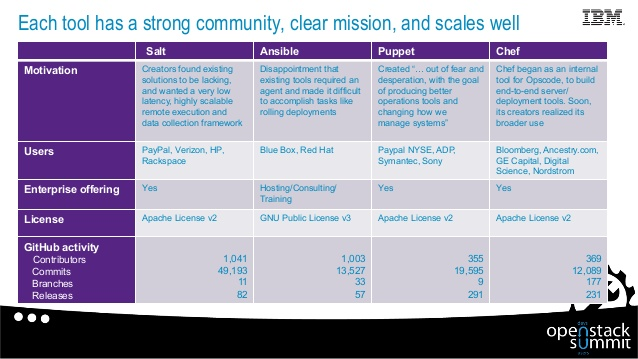
\includegraphics[scale=0.5]{images/configmanagement_tools1}
    \caption{Comparativa de herramientas de configuración, extraído de \href{https://www.slideshare.net/DanielKrook/caps-whats-best-for-deploying-and-managing-openstack-chef-vs-ansible-vs-puppet-vs-salt}{una charla de IBM}}
    \label{fig:configmanagement1}
  \end{figure}

\section{Arquitectura de la sonda}

A continuación, se incluye la arquitectura final de la sonda, que puede observarse en la figura \ref{fig:arquitectura-sonda}.

\begin{figure}[h]
    \centering
      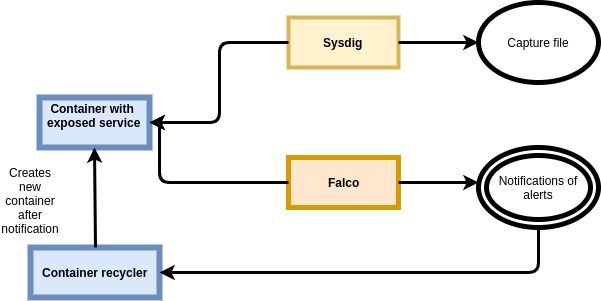
\includegraphics[scale=0.5]{images/probe_architecture}
    \caption{Arquitectura de la sonda}
    \label{fig:arquitectura-sonda}
  \end{figure}

\subsection{Elección del sistema operativo de la sonda}
\label{subsec:sonda-so}
  
La elección del sistema operativo tiene un componente en la que tendremos que tener en cuenta las capacidades del sistema operativo para su securización,
la existencia o no de actualizaciones de seguridad y las herramientas que incluye en su repositorio.

Para este proyecto se ha escogido GNU/Linux como sistema operativo por las herramientas que provee para gestionar nuestra \emph{honeypot} y su mejor soporte
para \emph{containers}. Así, habrá que escoger una distribución del sistema operativo que provea de actualizaciones de seguridad. Aunque la opción podría haber incluído \emph{CentOS, Container Linux, RHEL \ldots} o cualquier distribución con soporte, se ha escogido \emph{Debian} como distribución por ser la opción de referencia para servidores y mantener \emph{software} testado, con actualizaciones de seguridad, 
\emph{builds} reproducibles y por ser la distribución que más conoce y prefiere el autor.


\subsection{Creación del servicio expuesto}

Para la creación del servicio expuesto existen varias alternativas, pero no se puede olvidar que uno de los objetivos de este proyecto es el de utilizar \emph{containers} para describir nuestro servicio.

Como se explicó en 2.7, hay diversas tecnologías de ``contaneirización'', siendo \emph{Docker} la escogida por su madurez y conjunto de herramientas. 

\subsubsection{Elección del servicio a exponer}

La \emph{honeypot} puede albergar cualquier aplicación que se ejecute en un sistema Linux, servidores HTTP, aplicaciones
web, servidores FTP o cualquier otro tipo de servicio.

No todos los servicios tienen el mismo volumen de ataques ni el mismo interés, por ello, se escoge un servicio atractivo como SSH que 
expone el acceso a un servidor y capacita al atacante a realizar múltiples tipos de ataques.

\subsubsection{Gestionando el servicio expuesto en el \emph{container}}

Para gestionar el servicio expuesto, se ha creado un \emph{daemon} que se encargará de monitorizar que el \emph{container} esté siempre levantado, construir
la imagen y otras configuraciones. Para lanzar y mantener el estado del \emph{daemon}, se usa la funcionalidad existente en el gestor de procesos \emph{systemd}.

\emph{Systemd} es un sistema de arranque diseñado para reemplazar \emph{sysinit V} y \emph{upstart} (los sistemas de arranque clásicos) que ha sido adoptado
por las distribuciones principales tras generar resistencia y controversia.

    \begin{minted}[fontsize=\footnotesize]{console}
        [Unit]
        Description=Launch containers at startup
        
        [Service]
        Type=forking
        ExecStart=/usr/local/sbin/containersvc start
        ExecStop=/usr/local/sbin/containersvc stop
        Requires=docker.service
        RemainAfterExit=no
        Restart=always
        PIDFile=/var/run/containersvc.pid
        
        [Install]
        WantedBy=multi-user.target
    \end{minted}
    \captionof{listing}{Unidad de \emph{systemd} que gestiona el servicio \emph{containersvc} \label{listing:containersvc-systemd}
    }

Definiremos la unidad de \emph{systemd} (véase \cite{wiki-systemd}) listada como código \ref{listing:containersvc-systemd}. En ella se define el servicio \emph{containersvc} que requiere
que el servicio \emph{Docker} esté levantado (véase la directiva \emph{Requires}) y que será reiniciado siempre y cuando el servicio no exista (directiva \emph{Restart}). 
\emph{Systemd} conocerá el estado del servicio monitorizando el estado del proceso cuyo \emph{PID} se almacena en la ruta descrita en la directiva \emph{PIDFile}.

Básicamente, el servicio lanzará un \emph{script}, listado como código \ref{listing:containersvc-bash}, al que le pasará \emph{start} como argumento cuando arranque y, \emph{stop}
cuando pare.\ \\

    \begin{minted}[fontsize=\scriptsize]{console}
        #!/bin/bash
        ### BEGIN INIT INFO
        # Provides: containersvc
        # Required-Start: $local_fs $network $remote_fs
        # Required-Stop: $local_fs $network $remote_fs
        # Default-Start:  2 3 4 5
        # Default-Stop: 0 1 6
        # Short-Description: start and stop containers service
        ### END INIT INFO
        
        set -eufo pipefail
        
        DESC="container daemon"
        NAME="containersvc"
        PIDFILE="/var/run/containersvc.pid"
        touch $PIDFILE
        KPID=$(cat $PIDFILE)
        DOCKER_NETWORK="image_ssh"
        
        do_start() {
            touch $PIDFILE
            if [ -n "${KPID}" -a -d "/proc/${KPID}" ];then
              logger -t info [$NAME] $NAME already running
            else
              # cleanup unused and old docker images and volumes
              docker system prune -f
              cd /var/tmp/image
              export RANDOM_PASSWORD=$(shuf -n 1 /usr/share/dict/typical_passwords)
              export RANDOM_NAME=$(shuf -n 1 /usr/share/dict/words | tr -d "'")
              docker-compose up --build &
              echo $! > $PIDFILE
              sleep 10
              /usr/local/sbin/tc_manager.sh start $DOCKER_NETWORK
            fi
        }
        
        do_stop() {
         echo "Stopping $NAME";
         if [ -n "${KPID}" -a -d "/proc/${KPID}" ];then
             kill $KPID
             cd /var/tmp/image
             docker-compose stop
             # clearing up older iptables routes
             iptables -Z -t nat
             iptables -F -t nat
             /usr/local/sbin/tc_manager.sh stop $DOCKER_NETWORK
         fi
        }
        
        
        case "$1" in
           start)
             do_start
             ;;
           stop)
             do_stop
             ;;
           restart)
             do_stop
             do_start
             ;;
           *)
             echo "Usage: /etc/init.d/$NAME start|stop"
             exit 1
             ;;
        esac
        
        exit 0
    \end{minted}
    \captionof{listing}{Listado del servicio \emph{containersvc}      \label{listing:containersvc-bash}}

    
El \emph{script}, descrito como código \ref{listing:containersvc-bash}, realizará las siguientes acciones:

\begin{enumerate}
    \item Crear el fichero donde se almacenará el PID si no existe.
    \item Limpiar viejas imágenes y volúmenes antes de crear nuevos.
    \item Escoger una contraseña aleatoria como contraseña para los usuarios del servicio. Dicha
    contraseña se escoge de un listado de las 100 contraseñas más inseguras y reutilizadas, lo que aumenta
    la ratio de éxito para los atacantes en la explotación y permite aprender más.
    \item Escoger un nombre aleatorio como nomenclatura de máquina. Esto hace que el \emph{container} parezca un servicio
    más creible y que los atacantes no descarten la intrusión por detectar que están en un entorno construído para atraparles.
    \item Lanzar un proceso (\emph{docker-compose}, un orquestrador de órdenes de \emph{Docker} con un DSL propio) que crea la imagen del \emph{container}, una red propia para ese \emph{container} y lo lanza. 
    \item Lanza un proceso que limita el ancho de banda de red (se hablará más de ello en la sección \ref{subsec:securizacion-sonda}).
\end{enumerate}

La definición del \emph{docker-compose} se incluye como código \ref{listing:ssh-docker-compose}. En el fichero se puede ver que se expone el puerto
22 (puerto bien conocido para SSH), y que se le pasa el directorio actual para construir el \emph{container} y algunas variables de entorno 
creadas en el \emph{script} listado como código \ref{listing:containersvc-bash}.

    \begin{minted}[fontsize=\footnotesize]{console}
        version: "2"
        services:
          ssh:
            build:
              context: . #current dir as build context
              args:
                PASSWORD_GENERATED: ${RANDOM_PASSWORD}
            image: ssh
            ports:
              - "22:22"
            container_name: ssh
            hostname: ${RANDOM_NAME}
            domainname: superprivy.com
            networks:
              - ssh
        networks:
          ssh:
            driver: bridge
    \end{minted}
    \captionof{listing}{\emph{docker-compose} que crea el \emph{container} \emph{servicebase}     \label{listing:ssh-docker-compose}}

El fichero \emph{Dockerfile} que define la imagen, listado como 4, recoge la variable \emph{PASSWORD\_GENERATED} pasada como argumento al \emph{build} y utilizada para cambiar la contraseña
de dos usuarios del sistema. 

Como punto de entrada, se levanta el servicio SSH y se deja un proceso sin fin
corriendo (\emph{sleep infinity}) que es el que utilizará \emph{docker} para monitorizar el \emph{container} y será el proceso
número 1. Como no acaba nunca, el \emph{container} se ejecutará de manera continua. 
Esta imagen depende de otra, llamada \emph{servicebase}, cuya definición puede verse en el código \ref{listing:Dockerfile-base}. 
Esta permite que la creación de nuevos \emph{containers} sea muy rápida (aproximadamente de 1 segundo), ya que 
la imagen base contiene el sistema operativo y todas las utilidades ya descargadas y preparadas.

Si se quiere actualizar o cambiar la versión y/o incluir alguna utilidad, solo se ha de modificar el \emph{Dockerfile}
de la imagen base, cuya construcción será más lenta (del orden de minutos).

    \begin{minted}[fontsize=\footnotesize]{console}
        FROM servicebase:0.0.1
        ARG PASSWORD_GENERATED
        RUN echo "jeremy:$PASSWORD_GENERATED" | chpasswd
        RUN echo "root:$PASSWORD_GENERATED" | chpasswd
        RUN unset PASSWORD_GENERATED
        CMD /etc/init.d/ssh start && sleep infinity
        ENTRYPOINT /etc/init.d/ssh start && sleep infinity
        
    \end{minted}
    \captionof{listing}{\emph{Dockerfile} para SSH \label{listing:Dockerfile}}
    


\begin{minted}[fontsize=\footnotesize]{console}
    FROM debian:latest
    RUN useradd -ms /bin/bash jeremy
    RUN apt-get update
    RUN apt-get install -y rsyslog
    RUN apt-get install -y sudo
    RUN apt-get install -y ssh
    RUN apt-get install -y vim curl wget python perl build-essential
    RUN export HOSTNAME="$(sort -R /usr/share/dict/words | head -1 | tr -d \' )"
    RUN sed -i 's/PermitRootLogin without-password/PermitRootLogin yes/g' /etc/ssh/sshd_config
    CMD /etc/init.d/ssh start && sleep infinity
    ENTRYPOINT /etc/init.d/ssh start && sleep infinity
\end{minted}
\captionof {listing}{\emph{Dockerfile} base para imagen \label{listing:Dockerfile-base}}




\clearpage
\subsection{Obtención de trazas usando \emph{sysdig}}

Para obtener las trazas, se lanzará otro \emph{daemon} encargado de levantar \emph{sysdig} y de mantenerlo.
La definición de la unidad de \emph{systemd} se encuentra en el código \ref{listing:sysdig-systemd}. 

En resumen, se basa en lanzar un \emph{script} llamado \emph{sysdigd} (\emph{sysdig daemon}) que se monitoriza a través
del PID almacenado en el fichero descrito en la directiva \emph{PIDFile} y, siempre que el servicio
esté parado, se reiniciará como describe la directiva \emph{Restart}.

    \begin{minted}[fontsize=\footnotesize]{console}
        [Unit]
        Description=Launch sysdigd as daemon
        
        [Service]
        Type=forking
        ExecStart=/usr/local/sbin/sysdigd start
        ExecStop=/usr/local/sbin/sysdigd stop
        RemainAfterExit=no
        Restart=always
        PIDFile=/var/run/sysdigd.pid
        
        [Install]
        WantedBy=multi-user.target
    \end{minted}
    \captionof{listing}{Unidad de \emph{systemd} para controlar el \emph{daemon} de \emph{sysdig}   \label{listing:sysdig-systemd}}
\bigskip

El \emph{script} en sí, se lista como código \ref{listing:sysdig-bash}. Lo más relevante quizá
son las opciones que se pasan a \emph{sysdig}. Se hará una breve explicación de estas:
 \begin{minted}[fontsize=\footnotesize]{console}
        #!/bin/bash
        ### BEGIN INIT INFO
        # Provides: sysdigd
        # Required-Start: $local_fs $network $remote_fs
        # Required-Stop: $local_fs $network $remote_fs
        # Default-Start:  2 3 4 5
        # Default-Stop: 0 1 6
        # Short-Description: start and stop service sysdigd
        ### END INIT INFO
        
        
        DESC="sysdig daemon"
        NAME="sysdigd"
        PIDFILE="/var/run/sysdigd.pid"
        TRACES_DIR="/var/log/traces"
        KPID=$(cat $PIDFILE)
        
        do_start() {
            if [ ! -d /var/log/traces ];then
                logger -t info "creating traces directory"
                mkdir -p $TRACES_DIR &> /dev/null
        
            fi
        
            if [ -n "${KPID}" -a -d "/proc/${KPID}" ];then
                logger -t info [sysdigd] sysdig already running
            else
                logger -t info [sysdigd] launching sysdigd
                bash -c "sysdig -s 4096 -pc -F -C 200 -G 300 -W 5 -z \
                  -w /var/log/traces/$(hostname).%F-%H-%M.part > /dev/null 2>&1 &"
                sleep 5
                logger -t info [sysdigd] launched sysdigd
                PID=$(pidof sysdig)
                if [ -z "$PID" ];then
                    logger -t error [sysdigd] something went wrong, unable to launch sysdig
                    exit 2
                else
                    echo $PID > /var/run/sysdigd.pid
                fi
            fi
        }
        
        do_stop() {
         echo "Stopping $NAME";
             PID=$(pidof sysdig)
             if [ ! -z "$PID" ];then
                kill $PID
             fi
        }
        
        
        case "$1" in
           start)
             do_start
             ;;
           stop)
             do_stop
             ;;
           *)
             echo "Usage: /etc/init.d/sysdigd start|stop"
             exit 1
             ;;
        esac
        
        exit 0
    \end{minted}
    \captionof{listing}{\emph{Script} que controla \emph{sysdig}  \label{listing:sysdig-bash}}

\begin{itemize}
    \item \textbf{-s 4096}: define el espacio de almacenamiento de datos. Muchas \emph{syscalls} (como conexiones, escritura de ficheros) guardarán datos. Este parámetro define 
    cuantos datos se guardarán. Lo ideal para tener toda la información para su análisis sería guardar todos los datos, pero esto generaría trazas de longitud variable 
    y, posiblemente, de un tamaño que por su longitud sea complejo de gestionar (quizás se llenarían los discos de la sonda y se tardaría mucho tiempo en recolectar la traza o procesarla). 
    Definimos 4KiB por ser un tamaño adecuado para captar la mayoría de datos intercambiados y, de los obtenidos parcialmente, quizá capten también cierto conocimiento sobre ellos. 
    \item \textbf{-pc}: incluye en la salida información acerca de \emph{containers}, como la imagen del \emph{container}.
    \item \textbf{-F}: incluye todos los eventos, generando trazas más grandes pero más precisas.
    \item \textbf{-C 200}: rota el fichero de traza si el tamaño es superior a $200 * 10^6$ bytes.
    \item \textbf{-G 300}: rota el fichero de traza si el fichero actual es más antiguo de 300 segundos.
    \item \textbf{-W 5}: mantiene 5 ficheros de rotado. Junto a la opción \emph{-C} y \emph{G}, asegura que, en caso
    de recibir muchos eventos, las trazas seguirán siendo gestionables.
    \item \textbf{-z}: comprime el fichero de traza.
    \item \textbf{-w \emph{ruta}}: informa de en qué ruta se almacenan las trazas.
\end{itemize}

   

\subsubsection{Gestión del espacio de la sonda y eliminación de trazas}

Pese a que nuestro objetivo es mantener todas las trazas posibles, por razones puramente físicas,
el almacenamiento se acabará. Se necesita de algún proceso (listado como código \ref{listing:sysdig-cleanup-traces-script}) que se encargue de limpiar las trazas más antiguas, haciendo espacio
a las nuevas. Este proceso se debe lanzar con frecuencia, se ha configurado para ser lanzado cada 2 minutos en un \emph{Cronjob}.

Normalmente, este proceso no hará nada, pero si el espacio del punto de montaje seleccionado es menor del 10\%,
se preservarán las trazas más recientes (60 minutos desde que se ejecute, para dar margen al proceso de recolección de trazas) y se eliminarán el resto.

    \begin{minted}[fontsize=\footnotesize]{console}
        #!/usr/bin/env bash
        set -euo pipefail
        
        FREE_SPACE_THRESHOLD=10
        MOUNT_TO_WATCH="/"
        TRACES_DIR="/var/log/traces"
        LAST_MODIFIED_FILES_TO_KEEP_IN_MINUTES="60"
        
        
        get_free_disk_left() {
            percent=$(df -h ${MOUNT_TO_WATCH} --output=pcent | tail -1 | xargs | tr -d '%')
            FREE_SPACE=$((100-percent))
        }
        
        check_if_cleanup_is_needed () {
            if [[ $FREE_SPACE -le $FREE_SPACE_THRESHOLD ]]; then
                logger -t info "[cleanup] removing old traces"
                find $TRACES_DIR  -path "/var/log/traces/.ssh/*" -prune \
                -o -xtype f -mmin +$LAST_MODIFIED_FILES_TO_KEEP_IN_MINUTES -print0 | xargs -0 -L 50 rm
            fi
        }
        
        get_free_disk_left
        check_if_cleanup_is_needed
    \end{minted}
    \captionof{listing}{\emph{Script} que se lanza periódicamente para limpiar trazas. \label{listing:sysdig-cleanup-traces-script}    }
    

\subsection{Notificaciones usando \emph{falco}}

\emph{Falco} es una herramienta desarrollada por \emph{sysdig} que se encarga de monitorizar el comportamiento del sistema y de elaborar las notificaciones pertinentes en 
caso de que el sistema cumpla la regla descrita.

Sirva como ejemplo la siguiente regla:

\begin{minted}[fontsize=\scriptsize]{console}
    - rule: Run shell in container
    desc: a shell was spawned by a non-shell program in a container. Container entrypoints are excluded.
    condition: in_potted_container and spawned_process and container and shell_procs and proc.pname exists 
               and not proc.pname in (shell_binaries, docker_binaries, 
               k8s_binaries, initdb, pg_ctl, awk, apache2, falco, cron)
    output: "Shell spawned in a container other than entrypoint 
             (user=%user.name %container.info %container.info 
              shell=%proc.name parent=%proc.pname cmdline=%proc.cmdline)"
    priority: ALERT
\end{minted}
\captionof{listing}{Extracto de reglas de \emph{Falco}. \label{listing:extracto-falco}}
\bigskip

En ella se describe el título de la regla \emph{Run shell in a container}, una descripción de la regla y una condición que disparará la regla.
Si en un \emph{container } monitorizado se crea un proceso que no sea una \emph{shell} (el binario de \emph{docker}) o algunas herramientas conocidas
la condición se cumple y se dispará una notificación con la prioridad descrita (ALERTA).

Esta regla sirve para identificar cuando nuestra \emph{honeypot} de SSH ha sido vulnerada. Esta regla es un ejemplo de muchas
que ya vienen en el paquete de reglas base de \emph{Falco}. 

Para este proyecto se han realizado las siguientes modificaciones al conjunto de reglas base:

\begin{itemize}
    \item La identificación de las reglas que  marcan claramente que la \emph{honeypot} ha sido vulnerada
    y cambiar su prioridad al nivel maximo de ALERTA.
    \item La modificación de las macros y las reglas para escuchar eventos únicamente de los \emph{containers} que exponen servicios vulnerables.
\end{itemize}

Con estos cambios, \emph{Falco} se encarga de notificarnos cuando alguna de las condiciones descritas en estas reglas se cumplen.
Lo siguiente a realizar será actuar en base a estas notificaciones. En concreto necesitaremos las siguientes actuaciones:

\begin{enumerate}
    \item Registraremos las alertas en un fichero de \emph{log} que, posteriormente, será recolectado por el recolector vía \emph{rsyslog}.
    \item Necesitamos que, una vez detectada la intrusión, el atacante pueda actuar durante algún tiempo para obtener trazas pero,
    pasado este tiempo, se ha de parar el \emph{container}, borrarlo y crear uno nuevo desde una imagen limpia.
\end{enumerate}

Para la primera accion tenemos todas las herramientas necesarias porque solo utilizando \emph{rsyslog} ya se consigue el objetivo (véase \ref{subsubsec:usando-rsyslog}).
La segunda acción, sin embargo, es más compleja y exige de algún proceso que se encargue de, por un lado, escuchar las notificaciones de \emph{falco} y, por otro, de 
actuar en consecuencia, parando el \emph{container} en ejecución tras pasar el tiempo de exposición. 

\subsection{Gestor de \emph{containers} comprometidos en la sonda}


Para implementarlo, se crea una aplicación en \emph{Go} que realice estas funciones. Las razones para escoger \emph{Go} como lenguaje son:

\begin{enumerate}
    \item La concurrencia es soportada de una manera muy elegante y fácil a través de \emph{gorutinas} y canales.
    \item El compilador genera un binario estático que no requiere dependencias. En un entorno de seguridad como es este proyecto, esto
    tiene un gran valor ya que al no depender de bibliotecas dinámicas del sistema, reducimos la superficie de ataque.
    \item El hecho de que genere un único binario facilita la distribución e instalación de la aplicación que se reduce a copiar el fichero binario y darle permisos de ejecución.
\end{enumerate}

En el anexo \ref{subsec:containe-recycler-src-code} se listan algunos trozos de código de la aplicación. El encargado de lanzar el proceso será el propio
\emph{Falco}, como puede verse en el siguiente extracto de configuración:

\begin{minted}[fontsize=\scriptsize]{console}
    program_output:
    enabled: true
    program: "/usr/local/bin/container_recycler | tee -a /var/log/falco_alerts.txt"
\end{minted}
\captionof{listing}{Extracto de configuración de \emph{Falco}. \label{listing:config-falco}}
\bigskip


Cuando se recibe una notificación de tipo ALERT, el proceso deja el \emph{container} vivo durante algún tiempo (10 minutos) y tras ese tiempo, lo mata.

El servicio de \emph{containersvc}, descrito anteriormente (véase código \ref{listing:containersvc-bash}), detectará que el proceso ha sido matado
y creará un nuevo \emph{container}.

\begin{minted}[fontsize=\tiny]{console}
    time="2017-08-29T21:55:59Z" level=debug msg="ParseFalcoNotifications: received a falco notification" 
    time="2017-08-29T21:55:59Z" level=info msg="{21:55:58.886876283: Alert Shell spawned in a container other than entrypoint 
    (user=root ssh (id=fecb65acaf55) ssh (id=fecb65acaf55) shell=bash parent=sshd cmdline=bash -c #!/bin/sh
    PATH=$PATH:/usr/local/sbin:/usr/local/bin:/usr/sbin:/usr/bin:/sbin:/bin
    wget http://155.94.161.92/ys808e
    curl -O http://155.94.161.92/ys808e
    chmod +x ys808e
    ./ys808e
    ) Alert Run shell in container 2017-08-29 21:55:58.886876283 +0000 UTC}" 
    time="2017-08-29T21:55:59Z" level=debug msg="map[user:root image_name:ssh image_id:fecb65acaf55]" 
    time="2017-08-29T21:55:59Z" level=debug msg="Alert received, will try to stop container" 
    time="2017-08-29T21:55:59Z" level=debug msg="incomparable ID, provided ID is larger than existing one 
    time="2017-08-29T21:55:59Z" level=debug msg="FalcoNotification.handle: stopping container" 
    time="2017-08-29T21:55:59Z" level=info msg="scheduled container ssh for stopping" 
    time="2017-08-29T21:55:59Z" level=debug msg="ScheduleContainerStop: outside the lambda function waiting for DONE signal" 
    time="2017-08-29T22:05:59Z" level=info msg="Stopping container ssh NOW!" 
    time="2017-08-29T22:06:09Z" level=info msg="container ssh has been stopped" 
    time="2017-08-29T22:06:09Z" level=debug msg="ScheduleContainerStop: Lambda function DONE"     
\end{minted}
\captionof{listing}{Extracto de \emph{log} de \emph{container\_recycler}. \label{listing:container-recycler}}
\bigskip

\subsection{Securización de la sonda}
\label{subsec:securizacion-sonda}
Hay diversas medidas de seguridad a aplicar en la sonda. Siguiendo el principio de defensa en profundidad \cite{wikipedia-defense-in-depth}, aplicaremos diversas capas de protección en diferentes sistemas.

\subsubsection{Securización del sistema operativo}

En nuestro caso, la elección de \emph{Debian} permite utilizar capacidades como el sistema de \emph{unattended-upgrades} para actualizar paquetes del sistema cuando 
se publiquen actualizaciones de seguridad. 

Es recomendable seguir los estándares de la industria, como las guías de securización del \emph{CIS} o del 
\emph{NIST} (véase \cite{ovh-debian-cis} como ejemplo aplicado), que proporcionan guías de securización
para la mayoría de distribuciones y que son utilizadas para el cumplimiento de legislación que
gestiona datos sensibles como las tarjetas de crédito (PCI-DSS) (véase \cite{wiki-pci-dss}). 

\subsection{Reducción de la superficie de ataque}

Para ello, se deben eliminar servicios innecesarios de nuestro sistema y limitar el acceso a la red configurando un cortafuegos, que permita
el acceso solo a los puertos que deseamos desde los orígenes que deseamos.

\begin{minted}[fontsize=\scriptsize]{console}
    # {{ansible_managed}}
    iptables -P INPUT DROP
    iptables -P FORWARD ACCEPT
    iptables -P OUTPUT ACCEPT
    # las conexiones establecidas se mantienen.
    iptables -A INPUT -m state --state RELATED,ESTABLISHED -j ACCEPT
    iptables -A INPUT -i lo -j ACCEPT
    iptables -A INPUT -p icmp -j ACCEPT
    #servicio expuesto
    iptables -A INPUT -p tcp -m state --state NEW -m tcp --dport 22 -j ACCEPT
    #ssh de gestion
    iptables -A INPUT -p tcp -m state --state NEW -m tcp --dport 30009 -j ACCEPT
    
     
      iptables -A OUTPUT -p tcp -m state --state NEW -m tcp -o docker0 -d {{ ip }}/32 --dport 38080 -j REJECT
     
    
    
    iptables -A INPUT -j REJECT --reject-with icmp-net-unreachable 
    iptables -A FORWARD -j REJECT --reject-with icmp-net-unreachable     
    # Set up default policies
    
    ip6tables -P INPUT DROP
    ip6tables -P FORWARD DROP
    # we allow ipv6 output for updates
    ip6tables -P OUTPUT ACCEPT
    
    # Allow localhost traffic. This rule is for all protocols.
    
    ip6tables -A INPUT -s ::1 -d ::1 -j ACCEPT
\end{minted}
\captionof{listing}{Reglas de cortafuegos para sonda. \label{listing:cortafuegos-sonda}}
\bigskip

\subsection{Configuración del SSH de gestión}

Nuestra sonda expone el puerto tradicional de SSH para que sea atacado, pero aún necesita conectarse vía SSH para configurar el servidor,
instalar paquetes, etc.

Utilizamos \href{https://github.com/dev-sec/ansible-ssh-hardening}{un módulo de Ansible} para securizar el servicio SSH. 
Dicho módulo se encarga de:

\begin{itemize}
    \item Configurar el servicio para levantarse en otro puerto; en nuestro caso, el 30009. 
    La seguridad por oscuridad no aporta valor añadido pero reduce el número de ataques que recibimos. 
    \item Deshabilitar el uso de agentes SSH.
    \item Deshabilitar el inicio de sesión para \emph{root}.
    \item Deshabilitar el reenvío de tráfico a través de túneles TCP.
    \item Deshabilitar SFTP como servicio de transferencia, ya que puede ser usado para explorar el sistema de archivos del servidor.
    \item Configurar SSH para no usar algoritmos de cifrado débiles. 
\end{itemize}

\subsection{Securización del sistema de containers}

Las opciones de securización vienen condicionadas por haber escogido \emph{Docker} como sistema de ejecución de \emph{containers}
y \emph{Debian} como sistema operativo. 

En Linux podemos usar varios módulos del \emph{kernel} que implementan un sistema \emph{MAC (Mandatory Access Control)} en lugar de \emph{DAC (Discretionary Access Control)}. 
Básicamente, si el acceso es de tipo DAC (como el tradicional en sistemas unix) la capacidad o no de realizar una acción viene determinada por el actor que inicia la acción. Y las comprobaciones
para saber si puede ejercer la acción, el objeto sobre el que actúa se limitan a comprobar que sea dueño del mismo o el grupo al que pertenece el actor lo sea.
En un sistema \emph{MAC}, las políticas de qué está permitido o no involucran a los actores que inician la acción y los objetos sobre los que estos actuan -pudiendo limitar incluso al dueño del objeto a realizar ciertas acciones.

De los sistemas que implementan un control tipo MAC en linux, podemos enumerar como las principales alternativas:

\begin{itemize}
    \item \emph{SELinux}: desarrollado por la \emph{NSA} pero mantenido principalmente por \emph{Redhat}. Aunque está integrado como módulo de \emph{kernel},
    las herramientas y políticas solo se desarrollan y mantienen para distribuciones tipo \emph{Redhat} como \emph{RHEL,Fedora o CentOS} y derivadas de estas.
    El soporte de \emph{Debian} para \emph{SELinux}, aunque existe, no está mantenido oficialmente, lo que hace inviable esta opción. En SELinux los objetos (ficheros, conexiones de red) se identifican por
    un identificador que es invariable aunque la ruta al fichero cambie. 
    \item \emph{AppArmor}: desarrollado principalmente por \emph{SuSE Linux} y \emph{Canonical}, está integrado en el \emph{kernel} pero, al igual que \emph{SELinux}, 
    el soporte de herramientas y políticas existe principalmente en distribuciones \emph{SuSE}, \emph{Ubuntu} y \emph{Debian}. En AppArmor las políticas hacen referencia a rutas y no 
    a identificadores de fichero, lo que es una merma en las capacidades de securizar de \emph{AppArmor}.
    \item \emph{TOMOYO}: desarrollado por \emph{NTT Group}, parece que su uso y comunidad es muy pequeña, en comparación con las alternativas. Además, no está activamente mantenido. Similar a \emph{AppArmor} en filosofía.
    \item \emph{grsecurity}: es un conjunto de parches para el \emph{kernel} desarrollado por Brad Spengler de \emph{Open Source Security, inc}. Hasta Septiembre de 2015, se ofrecían parches al público de versiones estables y de pruebas del \emph{kernel}. 
    Despues de Septiembre de 2015, solo se ofrecían parches para versiones de prueba al público en general y para versiones estables para suscriptores de pago. En abril de 2017, también cerraron la descarga de parches
    para versiones de prueba. \emph{Grsecurity} ofrece el conjunto de parches y herramientas más completa y controvertida de las opciones a escoger. Instalar los parches de \emph{grsecurity} en un \emph{kernel}
    no garantiza la compatibilidad con aplicaciones existentes, sin embargo su control \emph{MAC} basado en roles y el conjunto de mejoras de seguridad al \emph{kernel}, la convierten en una opción atractiva de no ser por su modelo de distribución y sus problemas de compatibilidad.
\end{itemize}

Como resultado, escogeremos \emph{AppArmor} \cite{wiki-apparmor} para implementar nuestras políticas \emph{MAC}. \emph{Docker} soporta ser lanzado con perfiles de \emph{AppArmor} \cite{docker-doc-apparmor}, que permiten
limitar el conjunto de acciones que las aplicaciones podrán realizar \textbf{dentro} del \emph{container}. Existirán otros perfiles de \emph{AppArmor} que permiten limitar el comportamiento
de \emph{Docker} con el sistema que aloja \emph{containers}.
\ \\
\emph{Seccomp} \cite{wiki-seccomp} es una capacidad del \emph{kernel} que permite a procesos descartar privilegios de acceso a \emph{syscalls} 
que no necesitan. En el contexto de limitación de \emph{containers}, \emph{AppArmor} da un control más granular sobre qué se permite 
o no ejecutar a un \emph{container} mientras que \emph{seccomp} complementa 
la proteccion para acciones que no tengan sentido para ese \emph{container}.

\ \\
Por ejemplo, podemos restringir la \emph{syscall} \emph{sethostname} para un \emph{container} 
que ejecute un servidor web que difícilmente necesitará realizar esa operación.

\subsubsection{Limitación del ancho de banda usado por procesos que se ejecutan en \emph{containers}}

Cuando creamos el \emph{container} con el servicio expuesto, creamos una red propia para este \emph{container}. Puede verse
en el listado del código \ref{listing:ssh-docker-compose} en el apartado \emph{networks}.
\emph{Docker} crea un dispositivo de red virtual al que asocia un dispositivo \emph{bridge} virtual. Esto es necesario para que el 
\emph{container} tenga un \emph{namespace} \cite{wiki-namespaces} de red propio. Por defecto, a no ser que configuremos \emph{Docker}
de otra manera, se crearán reglas en \emph{iptables} para que este \emph{bridge} pueda salir a internet, y de esta manera los 
\emph{containers} que utilicen esta red tengan conexión a internet.
Esto es conveniente porque los \emph{containers} suelen necesitar acceso a la red -especialmente- si son servicios expuestos a clientes; pero en el caso de la \emph{honeypot}, pese a que deseamos que el atacante tenga
conexión a internet (muchos \emph{scripts} de atacantes si detectan que no hay conexión a internet, simplemente no hacen nada porque sospechan que 
están en una \emph{honeypot}), no queremos colaborar de manera activa con el ataque que se esté llevando a cabo.
La solución a esta aparente contradicción, es permitir el acceso a internet pero limitando la velocidad de la conexión a una tan baja que un ataque
dé tipo \emph{DDoS}.

Para ello, utilizaremos una herramienta llamada \emph{traffic control (tc)} (véase \cite{man-tc}) que nos permite manipular la gestión de trafico del \emph{kernel}
para nuestros dispositivos de red.

Como puede verse en el \emph{script} listado como código \ref{listing:tc-manager-script}, que se lanza desde el \emph{daemon} de gestión de \emph{containers} (código \ref{listing:containersvc-bash})
con la red de \emph{docker} del \emph{container} como argumento. La primera función del \emph{script} que gestiona \emph{tc} es (a partir de \emph{Docker}
averiguar a qué dispositivo \emph{bridge} pertenece y modificar las políticas de tráfico de dicho \emph{bridge}.
Respecto a las políticas de tráfico en concreto, reducimos el ancho de banda de descarga, y es subida a 56KiB y añadimos una latencia
de 50ms a la red. 

Se crean clases de tráfico, donde el tráfico SSH y el tráfico de diagnosis (ICMP) se marca como prioritario (priorizando la conexión del servicio expuesto),
el resto del tráfico se entregará con el ancho de banda disponible.


\begin{minted}[fontsize=\scriptsize]{console}
    #!/bin/bash -x
    
    clean_rules() {
        local iface=$1
        tc qdisc del dev $iface root    2> /dev/null > /dev/null
        tc qdisc del dev $iface ingress 2> /dev/null > /dev/null
    }
    
    start_traffic_shape(){
        local iface="$1"
        local maxbwidth_download="${2:-56}"
        local maxbwidth_upload="${3:-56}"
        local latency_added="${4:-50ms}"
        local burst_allowed="${5:-1540}"
    
        # clean existing down- and uplink qdiscs, hide errors
        tc qdisc del dev $iface root    2> /dev/null > /dev/null
        tc qdisc del dev $iface ingress 2> /dev/null > /dev/null
    
        ###### uplink
    
        # install root HTB, point default traffic to 1:20:
    
        tc qdisc add dev $iface root handle 1: htb default 20
    
        # shape everything at $UPLINK speed - this prevents huge queues in your
        # DSL modem which destroy latency:
    
        tc class add dev $iface parent 1: classid 1:1 htb rate ${maxbwidth_upload}kbit burst 6k
    
        # high prio class 1:10:
    
        tc class add dev $iface parent 1:1 classid 1:10 htb rate ${maxbwidth_upload}kbit \
        burst 6k prio 1
    
        # bulk & default class 1:20 - gets slightly less traffic,
        # and a lower priority:
    
        tc class add dev $iface parent 1:1 classid 1:20 htb rate $[9*$maxbwidth_upload/10]kbit \
        burst 6k prio 2
    
        # both get Stochastic Fairness:
        tc qdisc add dev $iface parent 1:10 handle 10: sfq perturb 10
        tc qdisc add dev $iface parent 1:20 handle 20: sfq perturb 10
    
        # TOS Minimum Delay (ssh, NOT scp) in 1:10:
        tc filter add dev $iface parent 1:0 protocol ip prio 10 u32 \
        match ip tos 0x10 0xff  flowid 1:10
    
        # ICMP (ip protocol 1) in the interactive class 1:10 so we
        # can do measurements & impress our friends:
        tc filter add dev $iface parent 1:0 protocol ip prio 10 u32 \
        match ip protocol 1 0xff flowid 1:10
    
        # To speed up downloads while an upload is going on, put ACK packets in
        # the interactive class:
    
        tc filter add dev $iface parent 1: protocol ip prio 10 u32 \
        match ip protocol 6 0xff \
        match u8 0x05 0x0f at 0 \
        match u16 0x0000 0xffc0 at 2 \
        match u8 0x10 0xff at 33 \
        flowid 1:10
    
        # rest is 'non-interactive' ie 'bulk' and ends up in 1:20
    
    
        ########## downlink #############
        # slow downloads down to somewhat less than the real speed  to prevent
        # queuing at our ISP. Tune to see how high you can set it.
        # ISPs tend to have *huge* queues to make sure big downloads are fast
        #
        # attach ingress policer:
    
        tc qdisc add dev $iface handle ffff: ingress
    
        # filter *everything* to it (0.0.0.0/0), drop everything that's
        # coming in too fast:
    
        tc filter add dev $iface parent ffff: protocol ip prio 50 u32 match ip src \
        0.0.0.0/0 police rate ${maxbwidth_download}kbit burst 10k drop flowid :1
    
    }
    
    get_bridge_docker_device(){
        local _outvar=$1
        local docker_network_name=$2
        local docker_network_id=$(docker network ls | grep $docker_network_name | cut -f1 -d' ')
        local result=""
        if [[ -z "$docker_network_id" ]]; then
            echo "unable to get bridge id from docker, refusing to continue, maybe it not exists?"
            result="NO_DEV"
            eval $_outvar=\$result
        return
        fi
        IFACE="br-$docker_network_id"
        ifconfig $IFACE &> /dev/null
        if [[ $? -ne 0 ]]; then
            echo "unable to contact bridged interface <$IFACE>, refusing to continue"
            result="NO_DEV"
            eval $_outvar=\$result
        return
        fi
        result="br-$docker_network_id"
        eval $_outvar=\$result
    }
    
    do_start() {
        local iface=""
        local docker_network_name=$1
        get_bridge_docker_device "iface" "$docker_network_name"
        if [[ "$iface" == "NO_DEV" ]]; then
          echo "unable to get interface, refusing to continue"
          exit 1
        fi
        clean_rules $iface
        start_traffic_shape $iface
    }
    
    do_stop() {
        local iface=""
        local docker_network_name=$1
        get_bridge_docker_device "iface" "$docker_network_name"
        if [[ "$iface" == "NO_DEV" ]]; then
          echo "unable to get interface, maybe it not exists"
          exit 0
        fi
        clean_rules $iface
    }
    
    do_status() {
        local number_of_rules=$(tc qdisc show | wc -l)
        if [[ $number_of_rules -gt 2 ]]; then
            echo "$0 is ENABLED"
        else
            echo "$0 is DISABLED"
        fi
    }
    
    
    case "$1" in
       start)
         do_start $2
         ;;
       stop)
         do_stop $2
         ;;
       restart)
         do_stop $2
         do_start $2
         ;;
       status)
         do_status
         ;;
       *)
         echo "Usage: /etc/init.d/$NAME start DOCKER_NETWORK_NAME | stop DOCKER_NETWORK_NAME | status"
         exit 1
         ;;
    esac
    
    exit 0    
\end{minted}
\captionof{listing}{\emph{tc\_manager} \emph{script} que controla ancho de banda usado en \emph{Docker} \label{listing:tc-manager-script}}
\bigskip


\section{Arquitectura del colector}
\label{sec:arquitectura-del-colector}


El servidor que realiza las funciones de recolector, también realiza las funciones
de \emph{backend} y \emph{frontend} de la API de clientes. La razón principal
es económica y, si la carga de la API o el almacenamiento disponible se queda pequeño,
habría que incorporar más servidores para la sostenibilidad del proyecto.

Igualmente, esta situación provoca una situación en la que este servidor se convierte en un 
punto de fallo y, si el servidor cae, la recolección de trazas y la API dejarán de funcionar.

Sin embargo, en el diagrama \ref{fig:arquitectura-general}, se recogen todos los procesos involucrados
en la recolección y la API, y su interacción con las sondas. Dicha interacción y relación no cambiaría pese
a que añadamos más servidores por razones de escalabilidad y resiliencia.

\begin{figure}[h]
    \centering
      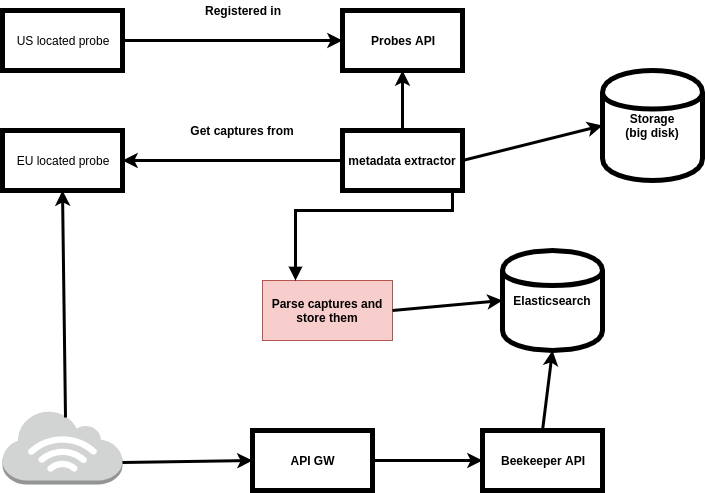
\includegraphics[scale=0.5]{images/collector_architecture}
    \caption{Diagrama de arquitectura del recolector}
    \label{fig:arquitectura-recolector}
  \end{figure}

\subsubsection{Microservicios}

El conjunto \textbf{NO} sigue una arquitectura de microservicios \cite{fowler-microservices}, pero sigue una arquitectura
orientada a servicios (SoA). En general cada elemento del diagrama \ref{fig:arquitectura-recolector} reune las siguientes
características:

\begin{itemize}
    \item Son desplegados en un \emph{container} y tiene un ciclo de vida independiente. Por ejemplo, se puede desplegar una nueva
    versión de \emph{metadata\_extractor} (el procesador de trazas) sin tener que desplegar otros componentes de la arquitectura
    siempre y cuando no haya cambios en la interfaz común entre componentes.
    \item Realizan una sola función o un número limitado de funciones bien definidas.
    \item Se asume que cada elemento puede compartir la red con otro elemento. Esto es así porque se lanzan en la misma máquina, y ayuda
    a simplificar la diagnosis en caso de problemas a costa de aumentar el acoplamiento.
    \item Existe acoplamiento entre elementos y esto va en contra de la arquitectura de microservicios.
    \item Se comparten bases de datos y esto también va en contra de la arquitectura de microservicios.
\end{itemize}

Creemos que no utilizar una arquitectura de microservicios es una decisión correcta para este caso, puesto que cambiar la arquitectura
actual a una de microservicios requeriría, posiblemente, la introducción de un \emph{backbone} de eventos o un sistema de colas y del despiece de la
base de datos y replicación para dotar a cada microservicio con su base de datos independiente.

Además, esto solo tendría sentido si el equipo técnico a cargo del proyecto fuese tan elevado que el coste de asumir esta arquitectura
(proceso de construcción independiente para cada servicio, test, definición de interfaces \ldots) lo justificase; y no es el caso.

\subsection{API de registro para las sondas}
\label{subsec:sinker-registry-api}

Como se comentaba en la descripción de riesgos de la sonda \ref{fig:riesgo_sonda}, las sondas son máquinas efímeras que se
crean y destruyen con cierta frecuencia, pero de las que necesitamos metadatos tales como el proveedor del servidor, 
la región geográfica en la que se encuentra o la dirección IP.

Por ello, necesitamos una API de registro donde se almacenen los datos de estas sondas. 

\subsubsection{Contrato de la API}

\begin{tabular}[!h]{|c|c|c|}
    \hline
    \thead{Verbo HTTP} & \thead{URL} & \thead{comentarios} \\
    \hline
    GET & /v1/probe/ & Listado de todas las sondas. \\
    \hline
    GET & /v1/probe/ip/:ip & Listado de sondas que tengan la IP :ip. \\
    \hline
    GET & /v1/probe/:id  & Listado de sondas que tengan el ID :id. \\
    \hline
    GET & /v1/probe/ssh/:id & Listado de claves SSH de la sonda con ID :id \\
    \hline
    GET & /v1/probe/name/:fqdn & Listado de sondas con el nombre DNS :fqdn \\
    \hline
    POST & /v1/probe & Crear una nueva sonda, el \emph{payload} puede verse en código \ref{listing:json-api-sinker} \\
    \hline
    PUT & /v1/probe/disable/:id & Deshabilitar la sonda con ID :id, no sale en listados \\
    \hline
    PUT & /v1/probe/enable/:id & Habilitar la sonda con ID :id \\
    \hline
    PUT & /v1/probe/tracespath/:id & Modificar directorio de trazas para sonda con ID :id \\
    \hline
    DELETE & /v1/probe/delete/:id & Eliminar sonda del registro con ID :id \\
    \hline
    \end{tabular}
    \captionof{table}{\label{tab:definicion-sinker-api} Definición de la api}
    

    \begin{minted}[fontsize=\footnotesize]{json}
        {
            ProbeID: "JyuU2_rTy2uU4x37Q_rURqpknnFX1VEWpZzhFg==",
            fqdn: "srv01.superprivyhosting.com",
            ipv4: "45.32.157.125",
            ipv6: "",
            provider: "Vultr",
            geolongitude: "8.728100",
            geolatitude: "50.117199",
            country: "Germany",
            sshprivateKey: "X",
            sshpublicKey: "Y",
            tracespath: "/var/log/traces",
            enabled: true,
            created_at: "2017-07-07T05:16:56.207424127Z",
            updated_at: "2017-07-21T09:50:18.528418195Z",
            disabled_at: "0001-01-01T00:00:00Z"
        }
    \end{minted}
    \captionof{listing}{Ejemplo de listado de una sonda en JSON de la \emph{Sinker Registry API} \label{listing:json-api-sinker}}

La API realiza las siguientes convenciones:

\begin{itemize}
    \item Cada identificador es único, no habrán dos sondas con el mismo identificador.
    \item Cada IP estará registrada a una sonda y a un nombre DNS, un mismo servidor no puede ofrecer más de una sonda (aunque sí, múltiples servicios).
    \item Aunque no está implementado, si se añadiera componente temporal se podrían habilitar, deshabilitar y consultar las sondas existentes por fecha además
    de por identificador, IP o nombre DNS.
\end{itemize}

\subsubsection{Clientes de \emph{Sinker Registry API}}

La API es de uso interno, es decir, no es visible desde el exterior, sino que solo es visible para las sondas y para el servicio de \emph{metadata\_extractor}.
Cuando la vía \emph{Ansible} se crea y se configura una nueva sonda, como parte del \emph{playbook} (listado de pasos para crear la sonda) se
realiza una llamada a la API para registrarla. Dicho proceso puede verse en detalle en el diagrama de secuencia UML \ref{fig:uml-sequence-post-probe}.
Si el registro ha sido exitoso la API devolverá un código 201 y un \emph{JSON} que incluye el ID de la sonda recién creada.

El diagrama de secuencia UML \ref{fig:uml-sequence-get-probe} muestra como se obtiene el listado de sondas a traves de su IP y la interacción
de diversos objetos.

\begin{figure}[htp]
    \centering
      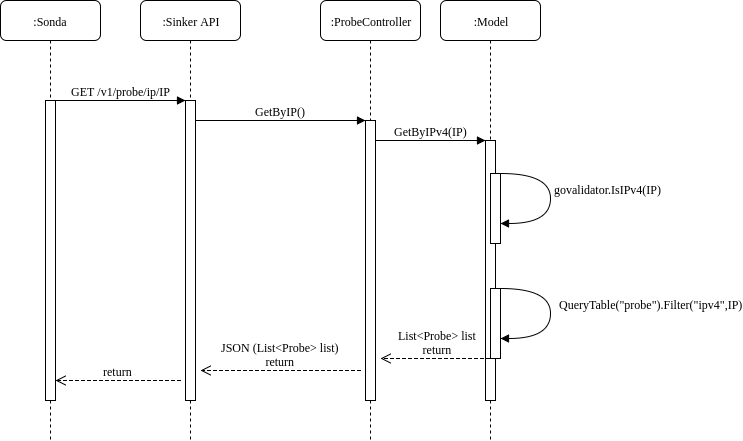
\includegraphics[scale=0.6]{images/UMLSequenceGetProbe}
    \caption{Diagrama de secuencia de UML de la API: GET}
    \label{fig:uml-sequence-get-probe}
\end{figure}

\begin{figure}[htp]
    \centering
      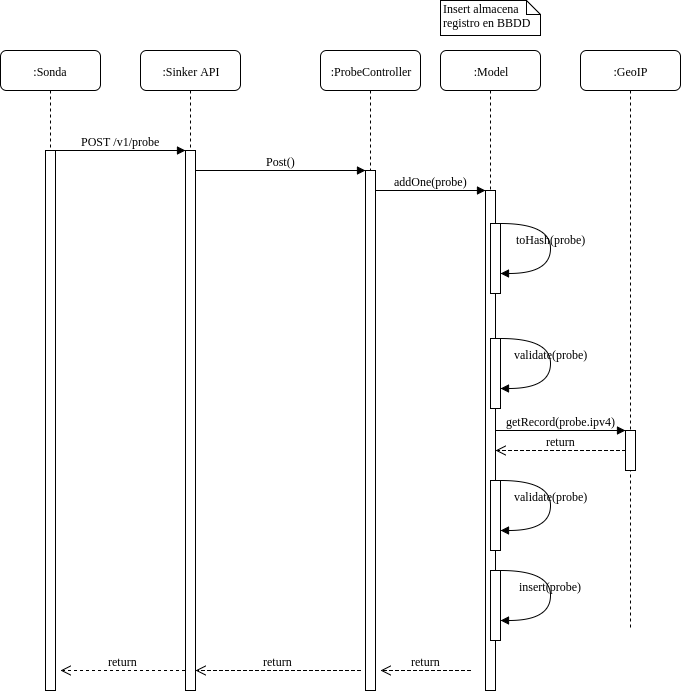
\includegraphics[scale=0.6]{images/UMLSequencePostProbe}
    \caption{Diagrama de secuencia de UML de la API: POST}
    \label{fig:uml-sequence-post-probe}
\end{figure}

\subsubsection{Implementación de la API}
\label{subsubsec:sinkers-registry-api-implementacion}

La API sigue el patrón MVC y se diseña como API REST, escogiendo \emph{Go} como lenguaje de programación para implementarla. Se escoge \emph{Go} 
como lenguaje para mantener la homogeneidad con otras herramientas del proyecto, para facilitar la reutilización de código,
por ser fácil de distribuir y desplegar (acaba siendo un binario estático) y por tener un muy buen soporte a la concurrencia y una biblioteca
estándar de HTTP muy versátil y potente.

Aunque la biblioteca estándar de \emph{Go} ya incluye un paquete de HTTP potente que se puede utilizar, se decide utilizar un \emph{framework} 
que permita la creación de la API de manera más rápida. Escogemos \emph{Beego} como \emph{framework} por ofrecer un \emph{ORM},
\emph{routers HTTP} y una \emph{CLI} para probar y desplegar la API entre otras funcionalidades y por ser simple y completo para nuestros
propósitos.

\subsection{Base de datos.}

Como se analizó en \ref{subsec:modelo-de-datos}, nuestra base de datos ha de reunir las siguientes características:

\begin{itemize}
    \item Orientada a búsquedas. La inserción se realizará con poco frecuencia, idealmente una sola vez (salvo reprocesados).
    \item Escalable y particionada. Como se analizó previamente, la información es menos relevante cuanto menos reciente sea, por lo tanto es importante
    ser capaces de particionar nuestra base de datos para albergarla completa por interés estadístico y ser capaz de eliminar una partición sin afectar al rendimiento del conjunto.
\end{itemize}

Por estas razones se escoge \emph{Elasticsearch} como base de datos. \emph{Elasticsearch} es una base de datos orientada a la búsqueda que permite
busquedas rápidas de texto y, la creación de series temporales.


\subsection{Extracción de datos y recolección de trazas}
\label{subsec:extraccion-trazas}

El servicio \emph{metadata\_extractor} se encarga de la recolección de trazas y de la extracción de datos de las mismas.
\emph{Metadata\_extractor} es una aplicación de consola escrita en \emph{Go} que depende de la API de sondas y, aunque puede prescindir de ella
en el proceso habitual, también depende de \emph{Elasticsearch}.

\begin{minted}[fontsize=\scriptsize]{console}
    ./metadata_extractor -h
    This silly application reads from sysdig traces from potted containers 
    and extracts data from them. It has
    two functioning modes, one that process capture files from arguments 
    and other that watches changes in filesystem through fanotify and process them
    
    Usage:
      metadata_extractor [command]
    
    Available Commands:
      file        sync files from ssh potted containers
      ssh         extracts metadata from ssh potted containers
    
    Flags:
      -c, --config string               config file (default is $PWD/.metadata_extractor.yaml 
                                            and $HOME/.metadata_extractor.yaml)
          --elasticsearch_host string   host to connect to elasticsearch
          --elasticsearch_port string   port to connect to elasticsearch
      -f, --follow                      follow traces created on fs, needs -i parameter
      -o, --output string               where to output between cli and es
      -i, --probeid string              probe id on sinkers API
      -s, --sinker_api_url string       sinker_api_url (default "http://main01.superprivyhosting.com:38080")
      -d, --tracebasepath string        Where the traces are stored  (default "/var/log/traces")
      -v, --verbose                     gives detailed logging
    
    Use "metadata_extractor [command] --help" for more information about a command.
\end{minted}
\captionof{listing}{Texto de ayuda de \emph{metadata\_extractor} \label{listing:metadata-extractor}}
\bigskip
\emph{Metadata\_extractor} puede leer de un fichero de configuración en lugar de ser pasado como uno de los argumentos descritos en la ayuda. En caso
de proporcionar ambos el argumento siempre tendrá prioridad.



% que es, es una CLI hecha en GoLang
% dos funciones principales, recoge trazas usando rsync, para eso consulta a la Sinker registry API donde hay
% claves ssh que puede usar para acceder al directorio de trazas.

% el otro es procesar las trazas, tienes dos modos o se le pasa como argumento una ruta y procesara los ficheros que encuentre
% o se le pasa u -f y procesara los ficheros que se vayan escribiendo en un directorio que escucha.
% los ficheros llegan a traves de fsnotify.

\subsubsection{Recolección de trazas}

\emph{metadata\_extractor} recolectará trazas si se le pasa como argumento el comando \emph{file}. Necesitará los siguientes
parámetros:

\begin{itemize}
    \item \textbf{-i}: Ya que cada sonda puede almacenar trazas en una ruta diferente, es necesario pasarle el 
                       identificador de la sonda para que \emph{metadata\_extractor} consulte en \emph{Sinker Registry API}
                       la ruta indicada y la clave SSH que utilizará para descargar las trazas. Para este fin,
                       las sondas crean un usuario denominado \emph{file} con únicamente permisos para leer trazas en las sondas, y
                       se crean claves SSH para dicho usuario que se publican en la API.
    \item \textbf{-s}: La URL donde la API de \emph{Sinker Registry} se encuentra, tiene un valor por defecto pero puede ser modificando
                       para realizar pruebas y/o para tener diversos entornos.
    \item \textbf{-d}: La ruta donde \emph{metadata\_extractor} escribirá las trazas recolectadas. Para guardarlas en el recolector
                       montamos un directorio del \emph{host} como volumen en \emph{Docker} (véase Código \ref{listing:metadata-extractor-docker-compose})
    \item \textbf{-b}: Límite de ancho de banda utilizado para descargar trazas.
\end{itemize}

En el diagrama de secuencia \ref{fig:uml-sequence-file-metadata-extractor}, se describe la operación de recolección y la interacción con la API de \emph{Sinker Registry}.

\begin{figure}[htp]
    \centering
      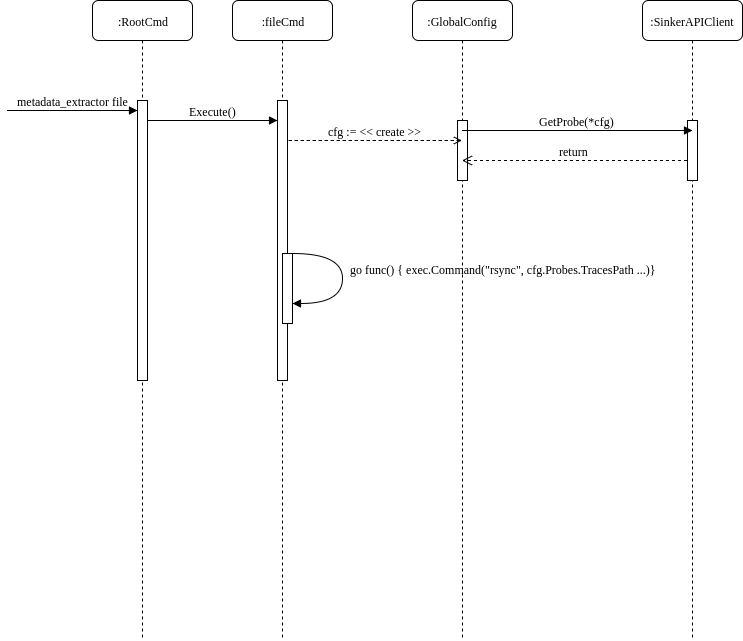
\includegraphics[scale=0.4]{images/UMLSequenceFileOp}
    \caption{Diagrama de secuencia UML del comando file de \emph{metadata\_extractor}}
    \label{fig:uml-sequence-file-metadata-extractor}
\end{figure}

\subsubsection{Procesando trazas de \emph{containers} \emph{SSH}}

El otro comando implementado en \emph{metadata\_extractor} es el procesado de trazas para extraer información relativa sobre
SSH, que es el protocolo que tenemos implementado en la \emph{honeypot}. El comando SSH utiliza los siguientes parámetros:

\begin{itemize}
    \item \textbf{-s}: Al igual que en para ficheros, la URL donde se encuentra desplegada la API.
    \item \textbf{-i}: El identificador de la sonda de la que procesaremos las trazas. Se necesita para consultar la API y obtener metadatos
    sobre la sonda que serán incluidos en el formato de salida de la traza. 
    \item \textbf{-f}: Este parámetro activa la escucha continua de eventos de creación de ficheros en la ruta definida por el parámetro \textbf{-d}. Básicamente, 
    se utiliza el subsistema \emph{inotify} (véase \cite{wiki-inotify}) del \emph{kernel} para recibir eventos de modificaciones en el sistema de archivos. Para cada
    evento de creación recibido, se intenta procesar la traza. Si no se pasa este parámetro, solo se procesarán los ficheros pasados como argumento.
    \item \textbf{-o}: donde se escribirán los datos extraídos, actualmente se implementan dos módulos de escritura, escritura a consola textual
    y escritura a la base de datos \emph{Elasticsearch}. En el caso de seleccionar esta última, hay que indicar dónde se encuentra la interfaz HTTP de \emph{Elasticsearch} y
    en qué puerto (\emph{--elasticsearch\_host} y  \emph{--elasticsearch\_port}). 
\end{itemize}

El detalle de la operación de extracción puede observarse en el diagrama de secuencia \ref{fig:uml-sequence-ssh-metadata-extractor} y en el código \ref{listing:metadata-extractor-handlers-ssh} listado en el anexo. 
El proceso de extracción de datos se basa en explorar la salida del proceso \emph{SSH}. \emph{SSH} es un protocolo de secreto perfecto (véase \cite{wiki-fsecrecy}) y
por tanto es imposible para nosotros interceptar la comunicacion entre cliente y servidor. La única opción para obtener la información de la comunicación es a través
de la memoria del proceso que realiza la función de servidor, el handicap de este enfoque es que no tenemos el contexto de la comunicación y no siempre podremos
mantener el orden cronológico de eventos.

Afortunadamente, podemos utilizar el orden cronológico de eventos de la CPU como indicador cronológico y la salida del proceso SSH que nos da información contextual. Lamentablamente,
esto implica que en un contexto determinado podemos superponer eventos y ordenarlos de manera incorrecta. El proceso que seguimos es:

\begin{enumerate}
    \item Ejecutamos \emph{sysdig} sobre la traza con un filtro más concreto para extraer la información que nos interesa. Por ejemplo, para extraer la información
    del intento de \emph{login} en el servicio \emph{SSH} (línea 230 del código \ref{listing:metadata-extractor-handlers-ssh}) o las ordenes ejecutadas en una sesión \emph{SSH} (línea 348 del código \ref{listing:metadata-extractor-handlers-ssh}).
    \item Analizamos la salida de \emph{sysdig} y obtenemos un listado de bloques de actividad y de \emph{login}. En el caso del \emph{login}, la salida nos devuelve
    el evento del intento de \emph{login}, su estado (si pudo iniciar sesión o no) y el nombre del usuario que realizó el intento. Sin embargo, la contraseña se lee de manera independiente puesto que el cliente 
    envia el \emph{challenge} usuario y contraseña, el servidor los comprueba y registra el resultado del intento de inicio de sesión. Al poder existir varios intentos de conexión de manera concurrente,
    tenemos que asegurarnos que no asociamos una contraseña a un usuario que intenta otra conexión. Para \emph{intentar} conseguir esto, ordenamos los eventos de \emph{login} por fecha e ID del hilo (línea 38 a 48 del código \ref{listing:metadata-extractor-handlers-ssh-models}) agrupándolos por el identificador del hilo del proceso (línea 93 a 103 del código \ref{listing:metadata-extractor-handlers-ssh}), 
    y analizamos los eventos recibidos intentando asociar contraseña con el usuario que realiza el intento. A veces, el usuario no envía contraseña: esto será marcado como `NOTPASSWORD` a la hora del análisis.
\end{enumerate}

Pese a que el proceso descrito puede parecer complejo, tiene la ventaja de que podemos analizar cualquier servidor SSH sin modificar el código del servidor SSH
lo que hace que este método, con sus limitaciones (no se obtienen las claves SSH que se intentan, a veces se pierde la contraseña del intento \ldots), sea potente y proporcione datos de interés.

Los datos extraídos se guardan en \emph{Elasticsearch} donde podrán ser consultados por otros servicios, en dos índices diferentes, uno para \emph{logins}
y otro para \emph{actividades}.

\begin{sidewaysfigure}[htp]
    \centering
    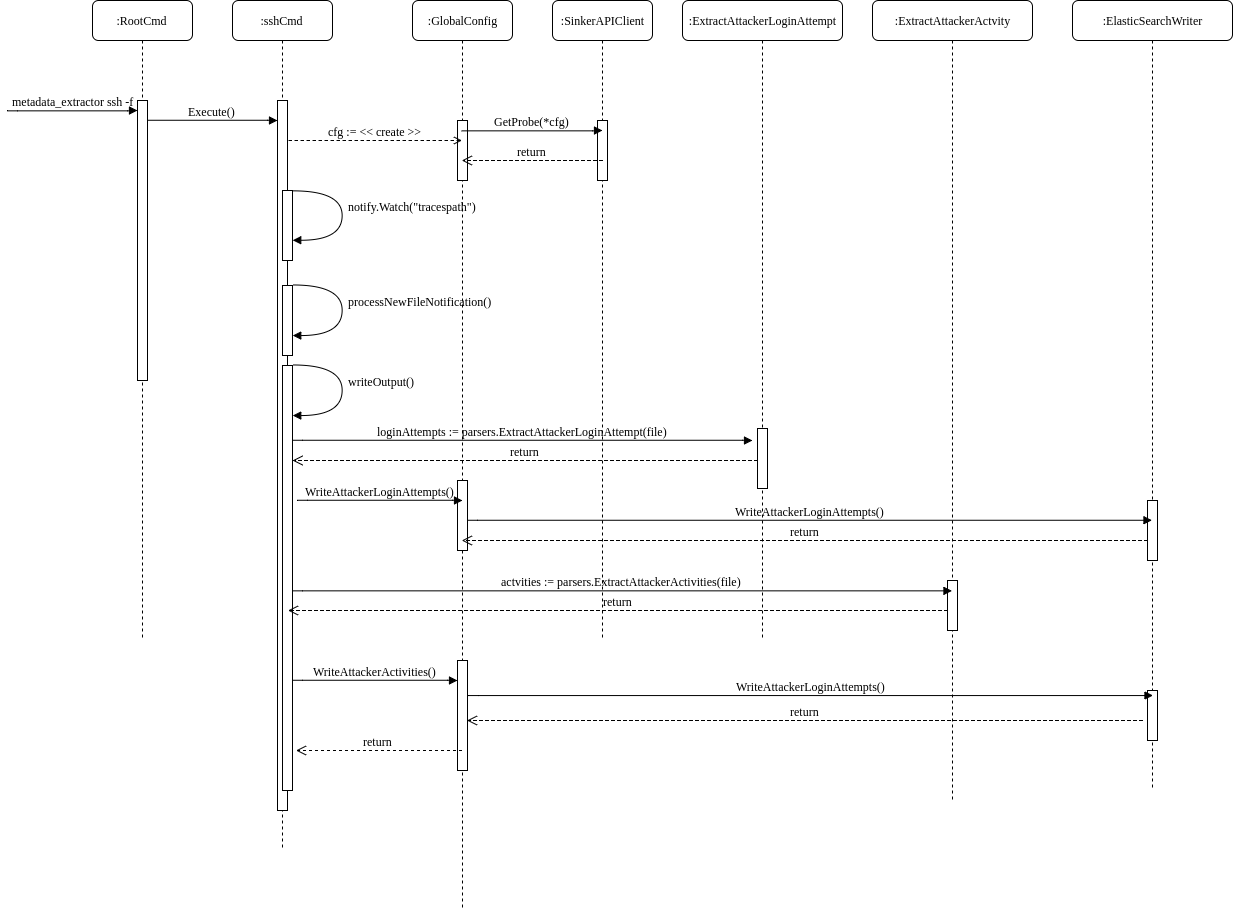
\includegraphics[scale=0.4]{images/UMLSequenceSSHOp}
    \caption{Diagrama de secuencia UML del comando SSH de \emph{metadata\_extractor}}
    \label{fig:uml-sequence-ssh-metadata-extractor}
\end{sidewaysfigure}

\subsubsection{Despliegue de metadata\_extractor}

Como en otros servicios ya explicados, creamos un \emph{daemon} que se encargará de lanzar los \emph{containers} del servicio \emph{metadata\_extractor}. Se ejecutan dos \emph{containers}
por cada sonda, uno que recolecta trazas y otro que las procesa. También se puede lanzar un \emph{container} de manera manual para reprocesar algunas trazas.

En el código \ref{listing:metadata-extractor-systemd}, puede verse la unidad de \emph{systemd} que define al \emph{daemon} y sus dependencias.
El \emph{daemon} se encarga de lanzar un \emph{script} similar al descrito en el código \ref{listing:containersvc-bash} que inicia el \emph{docker-compose}
descrito en el código \ref{listing:metadata-extractor-docker-compose}.


\begin{minted}[fontsize=\footnotesize]{console}
    [Unit]
    Description=Launch metadataextractor
    After=docker.service
    BindsTo=docker.service
    After=elasticsearchd.service
    BindsTo=elasticsearchd.service
    After=sinkerregistryapid.service
    BindsTo=sinkerregistryapid.service
    
    [Service]
    Type=forking
    ExecStart=/usr/local/sbin/metadataextractord start
    ExecStop=/usr/local/sbin/metadataextractord stop
    Requires=docker.service
    RemainAfterExit=no
    Restart=always
    PIDFile=/var/run/metadataextractord.pid
    
    [Install]
    WantedBy=multi-user.target    
         
\end{minted}
\captionof{listing}{Unidad \emph{systemd} que levanta el \emph{daemon} de \emph{metadataextractord} \label{listing:metadata-extractor-systemd}}
\bigskip


\begin{minted}[fontsize=\footnotesize]{console}
    version: "2"
    
    services:
      metadata_extractor_srv01_file:
        build:
          context: . #current dir as build context
          args:
            - CONFIGFILE=srv01metadataextractor.yaml
        image: metadata_extractor_srv01
        command: ./metadata_extractor -v file
        container_name: metadata_extractor_srv01_file
        network_mode: "host"
        restart: always
        volumes:
          - /var/log/traces:/var/log/traces
         
      metadata_extractor_srv01_ssh:
        build:
          context: . #current dir as build context
          args:
            - CONFIGFILE=srv01metadataextractor.yaml
        image: metadata_extractor_srv01
        command: ./metadata_extractor -v ssh -f
        container_name: metadata_extractor_srv01_ssh
        network_mode: "host"
        restart: always
        volumes:
          - /var/log/traces:/var/log/traces
         
\end{minted}
\captionof{listing}{\emph{Docker-compose} de \emph{metadata\_extractor} \label{listing:metadata-extractor-docker-compose}}
\bigskip

\subsection{Recolección de \emph{logs} y procesado de alertas}

Tal y como se describe en \ref{subsubsec:usando-rsyslog}, se guardan las alertas en un fichero de log que se recupera a través de
\emph{rsyslog}. 
Se instala el servidor \emph{rsyslog} en el recolector y clientes \emph{rsyslog} en las sondas, y se configura \emph{rsyslog}
para utilizar un canal cifrado para la comunicación mediante certificados SSL firmados por nuestra propia CA.

Una visión general del proceso puede verse en el diagrama \ref{fig:alert-log-architecture} con todos los componentes involucrados.

\begin{figure}[htp]
    \centering
    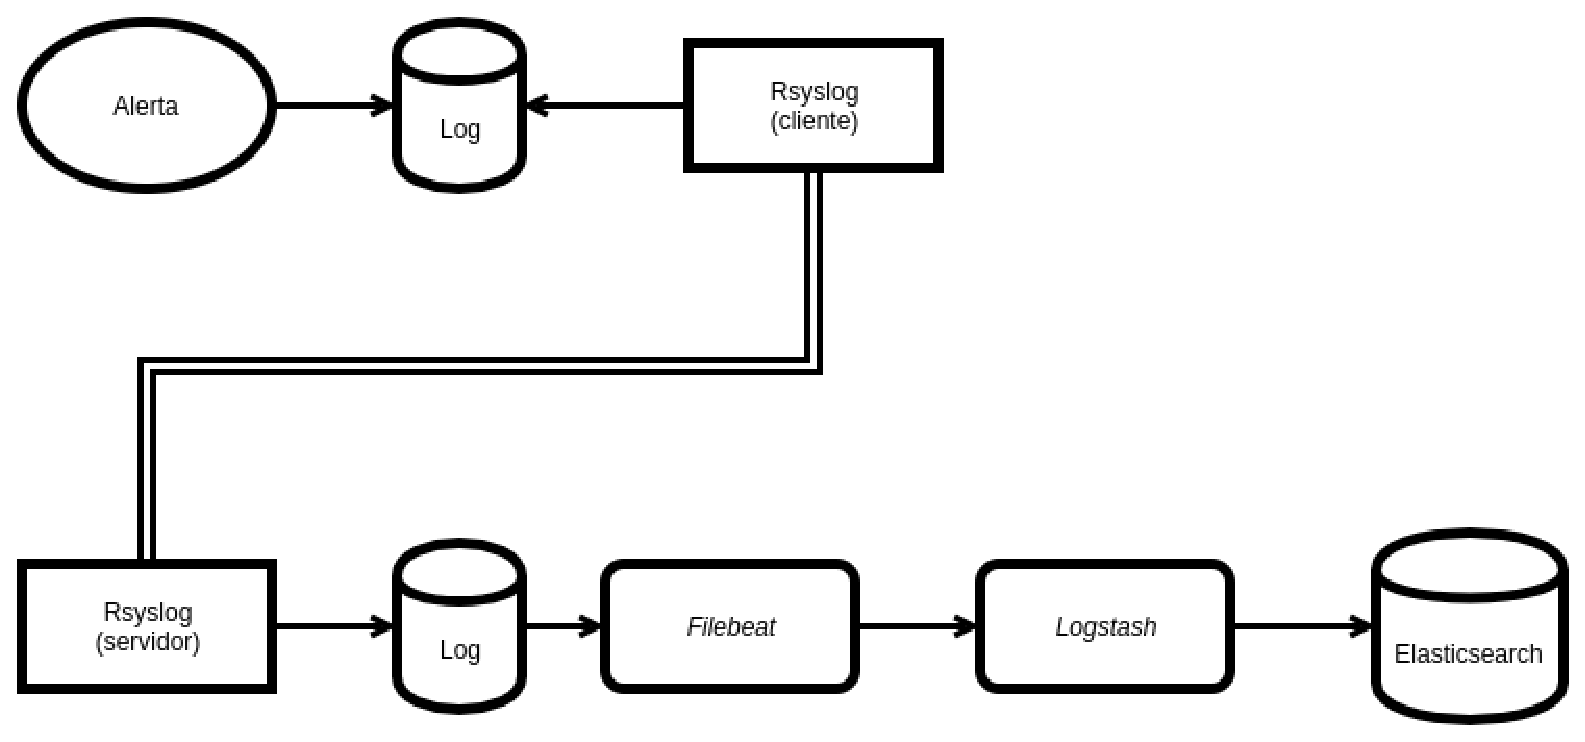
\includegraphics[scale=0.4]{images/AlertasEnvioLog}
    \caption{Diagrama de recolección de alertas y componentes involucrados.}
    \label{fig:alert-log-architecture}
\end{figure}

\begin{minted}[fontsize=\footnotesize]{console}
    # Increase the amount of open files rsyslog is allowed, which includes open tcp sockets
    # This is important if there are many clients.
    # http://www.rsyslog.com/doc/rsconf1_maxopenfiles.html
    - $MaxOpenFiles 2048

    # make gtls driver the default
    - $DefaultNetstreamDriver gtls

    - $DefaultNetstreamDriverCAFile {{ rsyslog_rsyslog_tls_ca_path }}
    - $DefaultNetstreamDriverCertFile {{ rsyslog_rsyslog_tls_cert_path }}
    - $DefaultNetstreamDriverKeyFile {{ rsyslog_rsyslog_tls_key_path }}

    # Provides TCP syslog reception
    # for parameters see http://www.rsyslog.com/doc/imtcp.html
    - module(load="imtcp"
           MaxSessions="2000"
           StreamDriver.mode="1"
          StreamDriver.authmode="x509/name"
           PermittedPeer="*.{{ pot_domain }}")
    - input(type="imtcp" port="10514" name="tcp-tls")
         
\end{minted}
\captionof{listing}{Configuración de \emph{rsyslog} como servidor. \label{listing:rsyslog-server}}
\bigskip

Desde el lado del cliente, en las sondas (como puede verse en el código \ref{listing:rsyslog-cliente}), se reenvían todos los logs
al recolector y solo a través del canal cifrado TLS. Se configura además un fichero en disco como almacenamiento temporal
para evitar pérdidas de alertas si hay problemas en la conexión de red.

\begin{minted}[fontsize=\footnotesize]{console}
    # make gtls driver the default
    - $DefaultNetstreamDriver gtls
    
    - $DefaultNetstreamDriverCAFile {{ rsyslog_rsyslog_tls_ca_path }}
    - $DefaultNetstreamDriverCertFile {{ rsyslog_rsyslog_tls_cert_path }}
    - $DefaultNetstreamDriverKeyFile {{ rsyslog_rsyslog_tls_key_path }}
    - $ActionSendStreamDriverAuthMode x509/name
    - $ActionSendStreamDriverPermittedPeer {{rsyslog_rsyslog_collector_dns_name}}
    - $ActionSendStreamDriverMode 1 # run driver in TLS-only mode
    - $WorkDirectory /var/spool/rsyslog # default location for work (spool) files
    - $ActionQueueType LinkedList # use asynchronous processing
    - $ActionQueueFileName srvrfwd # set file name, also enables disk mode
    - $ActionResumeRetryCount -1 # infinite retries on insert failure
    - $ActionQueueSaveOnShutdown on # save in-memory data if rsyslog shuts down
    - "*.* @@{{ rsyslog_rsyslog_collector_host_name}}:10514"         
\end{minted}
\captionof{listing}{Configuración de \emph{rsyslog} como cliente. \label{listing:rsyslog-cliente}}
\bigskip

Con ambas configuraciones conseguimos que los \emph{logs} de las sondas acaben en el \emph{rsyslog} del servidor.
El siguiente paso será filtar los eventos por sonda en ficheros diferentes. De otra manera, tendremos todos los eventos
en un unico log agregado en \code{/var/log/syslog}.

Para discriminar los \emph{logs} por servidor, utilizamos una funcionalidad de \emph{rsyslog} que nos permite
segregar los eventos por fichero en base a algunos parámetros, como puede verse en el código \ref{listing:rsyslog-split}.

\begin{minted}[fontsize=\footnotesize]{console}
     $ModLoad imuxsock.so
     $ModLoad imklog.so
     $ActionFileDefaultTemplate      RSYSLOG_TraditionalFileFormat
     $template DYNmessages,"/var/log/%HOSTNAME%/messages"
     $template DYNsecure,"/var/log/%HOSTNAME%/secure"
     $template DYNmaillog,"/var/log/%HOSTNAME%/maillog"
     $template DYNcron,"/var/log/%HOSTNAME%/cron"
     $template DYNspooler,"/var/log/%HOSTNAME%/spooler"
     $template DYNboot,"/var/log/%HOSTNAME%/boot.log"
     $template DYNfalco,"/var/log/%HOSTNAME%/falco.log"
     if $source != 'localhost' \
       and \
       $syslogseverity <= '6' \
       and ( \
         $syslogfacility-text != 'mail' \
         and \
         $syslogfacilitytext != 'authpriv' \
         and \
         $syslogfacility-text != 'cron' \
       ) \
       then    ?DYNmessages

     if \
          $source != 'localhost' \
          and \
          $syslogfacility-text == 'authpriv' \
       then    ?DYNsecure

     if \
          $source != 'localhost' \
          and \
          $syslogfacility-text == 'mail' \
       then    -?DYNmaillog

     if \
          $source != 'localhost' \
          and \
          $syslogfacility-text == 'cron' \
       then    ?DYNcron

     if \
          $source != 'localhost' \
          and \
          (\
            $syslogfacility-text == 'uucp' \
            or \
            $syslogfacility-text == 'news' \
          )\
          and \
          $syslogseverity-text == 'crit' \
       then    ?DYNspooler

     if \
          $source != 'localhost' \
          and \
          $syslogfacility-text == 'local7' \
       then    ?DYNboot

     if \
          $source != 'localhost' \
          and \
          $programname == 'falco' \
       then ?DYNfalco
\end{minted}
\captionof{listing}{Configuración de \emph{rsyslog} para segregar por fuente y servidor de origen. \label{listing:rsyslog-split}}
\bigskip

Con estas configuraciones, se consigue tener las alertas guardadas en disco en la ruta \code{/var/log/[SERVER\_NAME]/falco.log}. De modo que ahora, lo necesario será encontrar alguna manera enviar estas alertas a \emph{Elasticsearch} donde pueden ser correladas con los datos extraídos de las trazas.

\subsubsection{Envío de alertas a \emph{Elasticsearch}.}

Se necesita alguna aplicación que sea capaz de leer el fichero previamente mencionado que guarda \emph{rsyslog} y sea capaz de guardarlo
en \emph{Elasticsearch} lidiando con caídas de la base de datos, actualizaciones del fichero de \emph{log} y rotados.

Dicha aplicación no es especialmente compleja pero sí sensible. Afortunadamente, \emph{Elastic} la compañia que desarrolla principalmente
\emph{Elasticsearch} ya nos proporciona aplicaciones que realizan esta tarea:

\begin{itemize}
    \item \emph{Filebeat}: Se encarga de comprobar periódicamente si un conjunto de ficheros de origen ha sido modificado y, si lo han sido,
    enviar las modificaciones a \emph{Logstash} o directamente a \emph{Elasticsearch} entre otras opciones (véase \cite{elastic-filebeat}). Implementa 
    \emph{back-pressure}, si \emph{Logstash} o la salida seleccionada no confirma la escritura de nuevos eventos bajará paulatinamente la velocidad de envío. 
    Al enviarlas vía \emph{rsylog}, se añaden cabeceras a las alertas y, como necesitamos filtrar estas cabeceras para acceder a las alertas, necesitamos \emph{Logstash} para 
    guardarlas en \emph{Elasticsearch}.
    \item \emph{Logstash}: Se encarga de analizar el evento enviado por \emph{Filebeat}, de eliminar los sobrantes añadidos por \emph{syslog} y de realizar la inserción en
    \emph{Elasticsearch}.
\end{itemize}

\section{Arquitectura de la API de clientes}
\label{sec:arquitectura-api-clientes}

Con las sondas y el recolector funcionando, la siguiente tarea a realizar es poner en marcha la API de clientes, 
la API que se usará para extraer información de incidentes de manera correlada.

La API es sencilla y su contrato ya fue descrito en \ref{subsubsec:definicion-api}. En este caso, por falta de tiempo no se implementa
la función de \code{/feed} y solo se oferta el protocolo SSH.

La API depende de \emph{Elasticsearch}. Si \emph{Elasticsearch} no funciona la API no puede obtener las alertas ni los datos de capturas y no funcionará. Para reducir el acoplamiento entre la base de datos y la API, habría que implementar una caché 
en la API y/o incluir una base de datos propia del servicio para seguir una arquitectura de microservicios. Ninguna de estas opciones se ha implementado en la versión actual.


La API está abierta a Internet y, por lo tanto es susceptible a ataques del exterior ya sea de denegación del servicio o de intentos de intrusión. 
Para mitigar el riesgo de intrusión sería conveniente aislar la API en un servidor propio, pero esto aumentaría el coste económico del proyecto, dado 
que la API es sencilla e implementada en \emph{Go}, se asume el riesgo de intrusión.

El riesgo de denegación de servicio sigue presente y la manera de mitigarlo es implementar políticas de contención de tráfico.


\subsection{Inclusión de un \emph{API Gateway} }

Aunque podríamos implementar políticas de \emph{rate-limiting} en la propia API, se decide externalizar a un \emph{API Gateway}, una API para APIs que ofrece funciones genéricas como
autenticación, control de tráfico, cuotas, cacheo y otros. 

Utilizar un \emph{API Gateway} también permite separar nuestra API en diversos servicios cuando sea necesario especializar alguna de las funciones
. Por ejemplo, externalizar la función de \code{/feed} de la API a otro servicio. 

Se decide usar \emph{krakend} (\href{http://www.krakend.io/}{http://www.krakend.io/}) como \emph{API Gateway} por ser simple, \emph{Open Source} y útil para este propósito aunque se podría utilizar cualquier otra. En concreto, 
\emph{krakend} se encargará del \emph{rate-limit} y de la terminación \emph{SSL}. Para obtener los certificados hacemos uso de la iniciativa del Internet Security Research Group \emph{Let's Encrypt} que nos
ofrece certificados \emph{TLS} validados por una \emph{CA} pública de manera gratuita.

\subsection{Diseño de la API}

La API se implementa en \emph{Go} utilizando el \emph{framework Beego} al igual que la API de registro de sondas descrita en el apartado \ref{subsubsec:sinkers-registry-api-implementacion}, 
por las razones allí expuestas y para reaprovechar código entre ellas.

Por razones de tiempo, solo se ha podido implementar el \emph{endpoint} de incidentes. Se trata fundamentalmente de crear un objeto
que relacione alertas recibidas con intentos de \emph{login} y actividades detectadas en la sonda si existen. El código \ref{listing:beekeeper-api-models-ssh-incident}, 
líneas 117 a 127, muestra cómo se construye dicho objeto combinando tres índices de \emph{Elasticsearch}: el índice de alertas, con el de \emph{activities} y, por último, el \emph{login-attempts}.
con información de la sonda utilizando la API de registro de sondas.

\subsection{Salida de la API}

El código \ref{listing:api-incident-json} muestra un ejemplo del JSON que devuelve la API que representa un incidente. En la estructura se 
incluyen los siguientes campos:

\begin{itemize}
    \item \code{started\_at}: fecha de inicio del incidente.
    \item \code{finished\_at}: fecha de fin del incidente, a veces es imposible de determinar y se establece a la fecha nula (\code{0000-00-00T00:00:01Z}).
    \item \code{ID}: identificador del incidente.
    \item \code{Activities}: Listado de actividades (órdenes lanzadas) detectadas en la sonda.
    \item \code{Offenders}: Listado de atacantes que intentaron y/o consiguieron iniciar sesión en la sonda en la ventana de tiempo del incidente. Se incluye además la IP de atacantes y geolocalización.
    \item \code{Provider}: Proveedor en qué esta instalada la sonda.
    \item \code{Triggered}: Mensaje de la alerta que inicia el incidente.
\end{itemize}

Con esta información expuesta, los clientes pueden crear sus propias herramientas de visualización y respuesta a incidentes. Es importante destacar que 
el incidente tiene un marco temporal y que se debe actuar teniéndolo en cuenta. Por ejemplo, una determinada IP puede realizar una actividad maliciosa en un 
periodo de tiempo y ser legitima posteriormente (por ser parte de una \emph{botnet}, porque el servidor infectado ha sido destruído y la IP asignada a otro servidor, etc).

\begin{minted}[fontsize=\footnotesize]{json}    
{
    Activities: [
    {
    @timestamp: "2017-09-01T01:15:07.143824471Z",
    activity: "bash -c uname -a",
    containerid: "6d7e2680e0d3",
    pid: "20855",
    user: "root"
    }
    ],
    Country: "Germany",
    FinishedAt: "2017-09-01T01:24:40Z",
    ID: "1504228507000-Vultr",
    Offenders: [
    {
    @timestamp: "2017-09-01T01:24:40Z",
    containerid: "6d7e2680e0d3",
    country: "Czech Republic",
    ip: "91.195.103.215",
    location: {
    lat: 50.071201,
    lon: 14.2758
    },
    password: "123456 ",
    successful: true,
    user: "root "
    }
    ],
    Provider: "Vultr",
    StartedAt: "2017-09-01T01:15:07.143818446Z",
    Triggered: " Alert Shell spawned in a container other than entrypoint 
    (user=root ssh (id=6d7e2680e0d3) 
    ssh (id=6d7e2680e0d3) 
    shell=bash parent=sshd cmdline=bash -c uname -a)"
},
\end{minted}
\captionof{listing}{Ejemplo de incidente expuesto en la API \label{listing:api-incident-json}}
\bigskip


\section{Análisis de datos obtenidos a través de la \emph{honeypot}}

Esta sección demuestra el tipo de visualizaciones que se pueden obtener a través de la API de clientes para obtener
patrones y datos sobre atacantes. Todas las visualizaciones comprenden el periodo del 4 de Junio de 2017 al 2 de Septiembre de
2017 (90 días).

En la figura \ref{fig:data-alerts-by-day} podemos ver una gráfica de las alertas generadas. Se puede observar que hay un pico de 
alertas alrededor del 7 de Julio que también se ve reflejado en la figura \ref{fig:data-attempts-per-provider} donde se muestran
los intentos de inicio de sesión por día y proveedor.
    Se puede apreciar en ambos que la actividad maliciosa es continua en el tiempo pero con intensidad variable. Si nos detenemos en la figura \ref{fig:data-attempts-per-provider} también podemos observar
 que un proveedor es más atacado que otro, esto puede guardar relación con las diferencias
perimetrales del proveedor.

En la figura \ref{fig:data-table-by-country-unified} hay una tabla con los países que originan más ataques desde IPs diferentes (no se tiene en cuenta 
la repetición de ataques desde la misma IP) que puede observarse de una manera más visual en la figura \ref{fig:data-map-unified}. Como vemos los ataques son globales,
pese a que hay países como China, Argentina o Rusia que generan más ataques que el resto.

Si nuestro servicio está localizado en varios países y no incluye a los tres mencionados una posible respuesta sería bloquear todo el tráfico proveniente
de estos países, lo que es una medida muy drástica pero efectiva. 

En la figura \ref{fig:data-pie-passwords} pueden observarse los usuarios habitualmente utilizados (círculo interno) con respecto
a las contraseñas más utilizadas. Vemos que el usuario \code{root}, seguido de \emph{admin} es el más utilizado y que en contraseñas
\code{1234} y \code{password} son de las más utilizadas.

Podemos observar tambien en la figura \ref{fig:data-pie-passwords-successful}, las contraseñas y usuarios que tuvieron exito en las que podemos ver
como el usuario \code{root} predomina y las contraseñas \code{12345}, \code{123456} y \code{111111} son las más utilizadas.

Dicha distribución tiene sentido ya que nuestras sondas tienen solo dos usuarios \code{jeremy} y \code{root}, y se utiliza una contraseña aleatoria 
de la siguiente lista:

\begin{table}[h]
    \centering
    \begin{tabular}[!h]{|l|}
        \hline
        
        \thead{Contraseñas de las sondas} \\
        \hline
        root \\
        \hline
        123456 \\
        \hline
        password \\
        \hline
        12345678 \\
        \hline
        123456789 \\
        \hline
        12345 \\
        \hline
        1234 \\
        \hline
        111111 \\
        \hline
        1234567 \\
        \hline
        123123 \\
        \hline
        abc123 \\
        \hline
        696969 \\
        \hline
        shadow \\
        \hline
        master \\
        \hline
        666666 \\
        \hline
        1234567890 \\
        \hline
        654321 \\
        \hline
        7777777 \\
        \hline
        000000 \\
        \hline
    \end{tabular}
    \caption{\label{tab:sondas-passwords}Contraseñas de las sondas.}
    \end{table}

Durante la construcción del prototipo, se probó a crear sondas que permitían iniciar sesión SSH sin contraseña. 
Pero al hacerlo se comprobó que:

\begin{itemize}
    \item La mayoría de atacantes son scrips automatizados, si no se les pregunta por contraseña asumen que es una \emph{honeypot} y no realizan ninguna actividad.
    \item Perdemos la información del login, puesto que no vemos que combinaciones se han probado para iniciar sesión ni cúales son las más exitosas.
\end{itemize}

Por estas razones se decide utilizar el listado expuesto en el cuadro \ref{tab:sondas-passwords}, extraído de un repositorio que incluye las contraseñas
más utilizadas según análisis de volcado de contraseñas de sitios web conocidos (\href{https://github.com/danielmiessler/SecLists.git}{https://github.com/danielmiessler/SecLists.git}).

De estos diagramas podemos extraer que si no permitimos que el usuario \emph{root} inicie sesión, eliminamos de un plumazo un porcentaje importante de ataques.

Lamentablamente lo más interesante sería analizar los ficheros utilizados dentro de la \emph{honeypot} pero no ha sido implementado por falta de tiempo. Es una tarea
que es factible pero no fácil y que, pese a todo podemos implementar usando la API, extrayendo las \emph{urls} de descarga y analizando el fichero descargado en plataformas como
\emph{VirusTotal}.

Lo interesante de este enfoque sería poder ofertar datos estadísticos de los tipos de \emph{malware} que observamos en la \emph{honeypot} y ser capaces de determinar si se encuentra un malware por
su actividad que no sea reconocido en plataformas de análisis de muestras.

Durante el tiempo que el sistema lleva funcionando, se ha observado que la \emph{honeypot} ha sido infectada para formar parte de una \emph{botnet Mirai} (véase \cite{wiki-mirai})
o para ser parte de una \emph{botnet} que realiza ataques DDoS a la plataforma de Sony Playstation.

Es ahí donde reside el potencial más interesante de la \emph{honeypot}, pese a que la información que ya se extrae es valiosa por sí misma.

\begin{sidewaysfigure}[h]
    \centering
      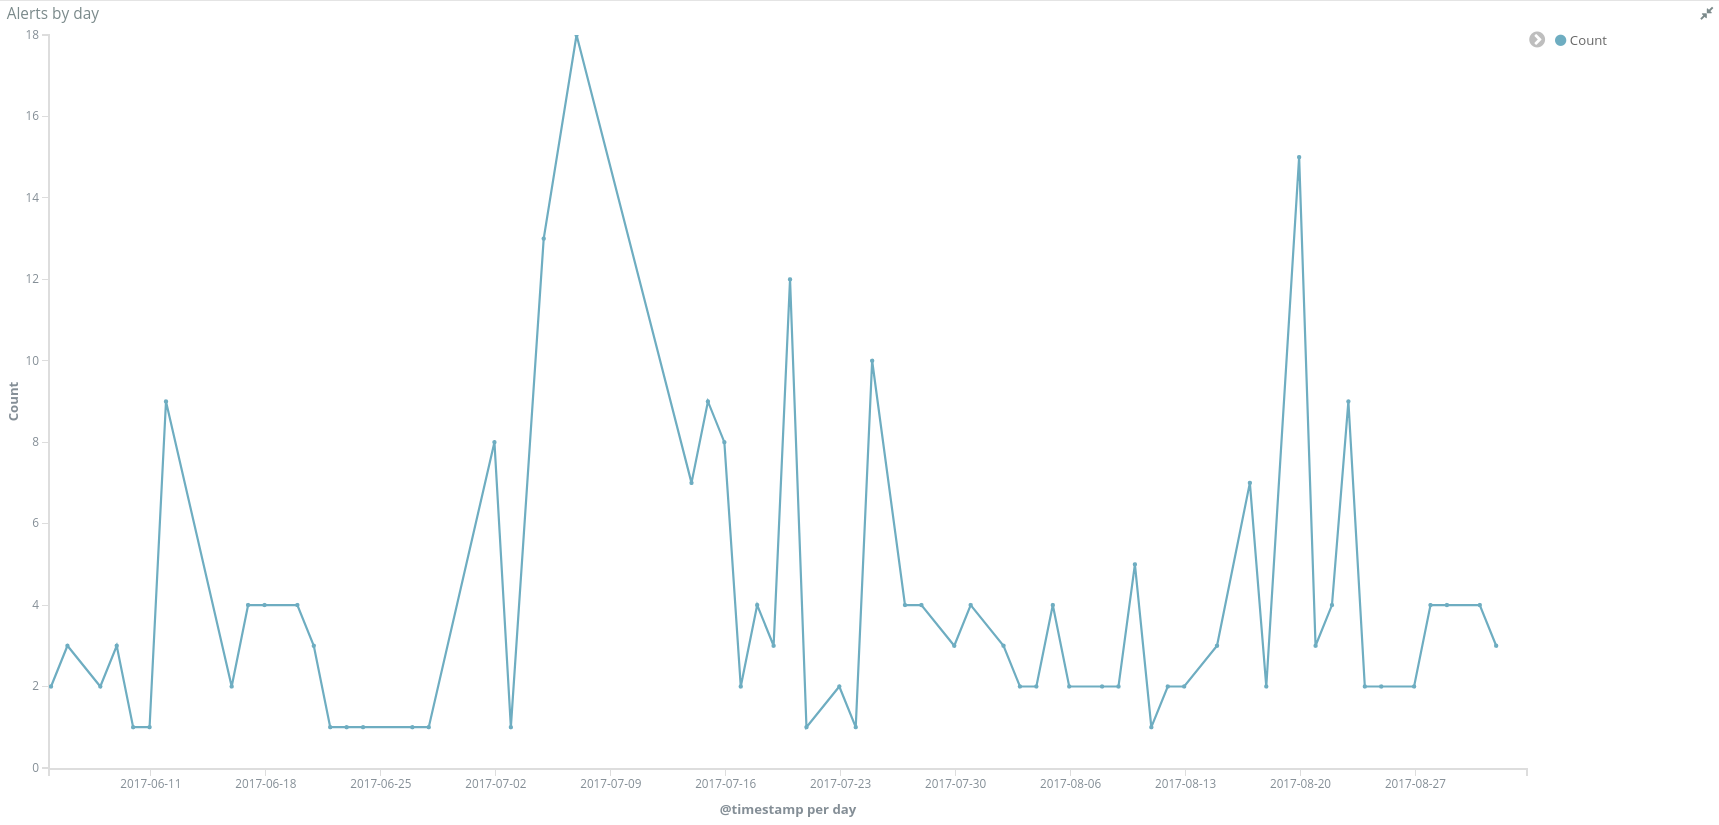
\includegraphics[scale=0.3]{images/ElasticAlertsByDay}
    \caption{Alertas generadas por las sondas en el periodo del 4 de Junio de 2017 al 2 de Septiembre de 2017.}
    \label{fig:data-alerts-by-day}
  \end{sidewaysfigure}

  \begin{sidewaysfigure}[h]
    \centering
      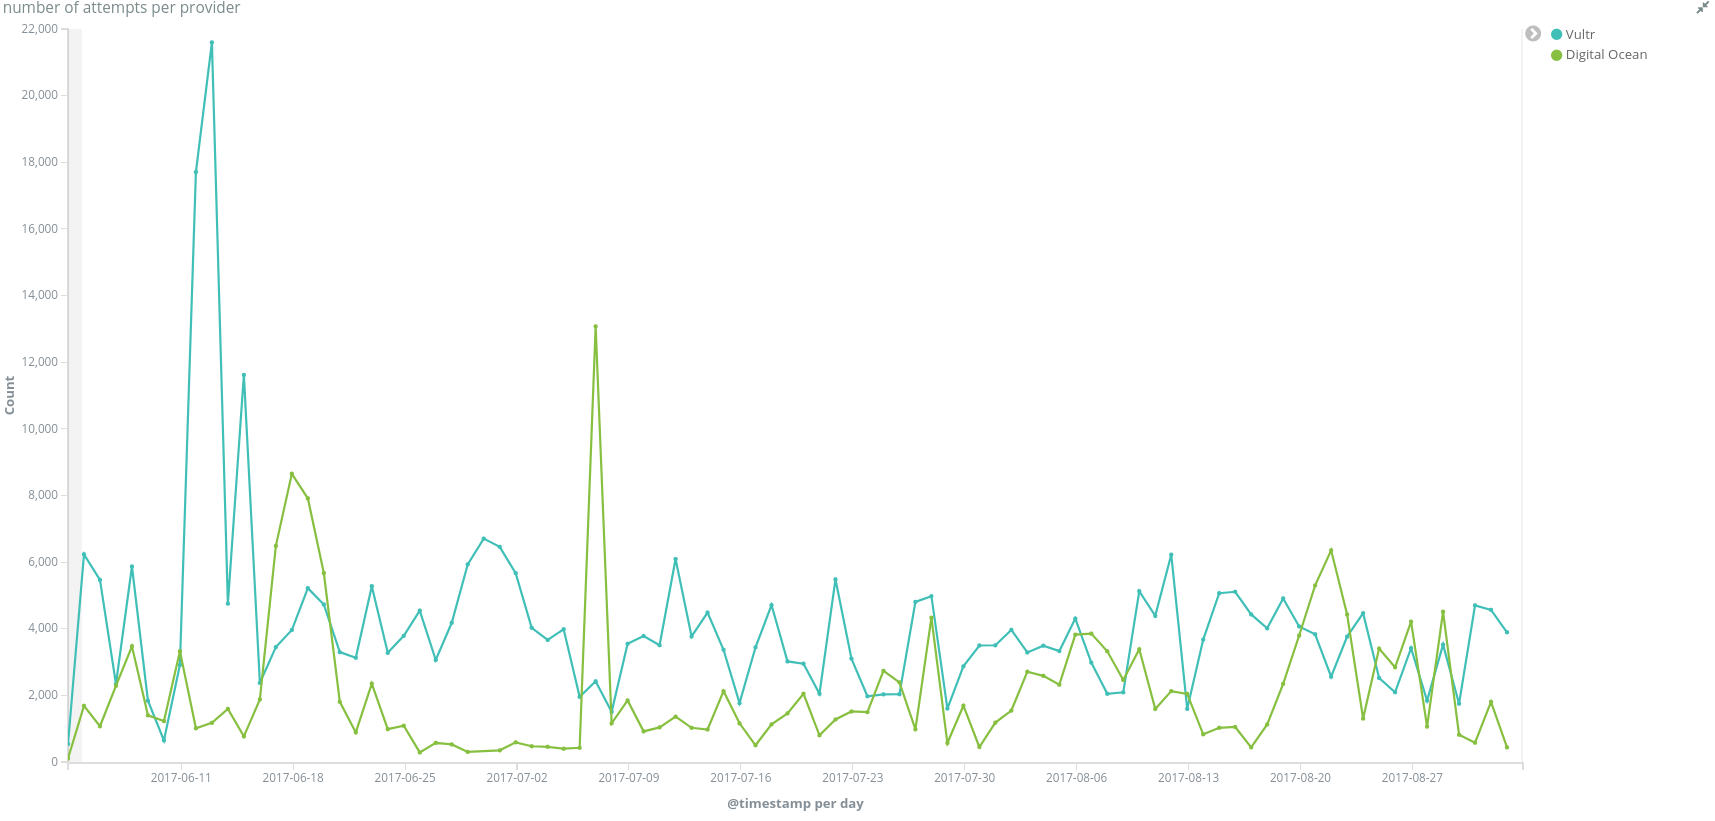
\includegraphics[scale=0.3]{images/ElasticAttemptsPerProvider}
    \caption{Intentos de \emph{login} en el periodo del 4 de Junio de 2017 al 2 de Septiembre de 2017 por proveedor.}
    \label{fig:data-attempts-per-provider}
  \end{sidewaysfigure}

  \begin{sidewaysfigure}[h]
    \centering
      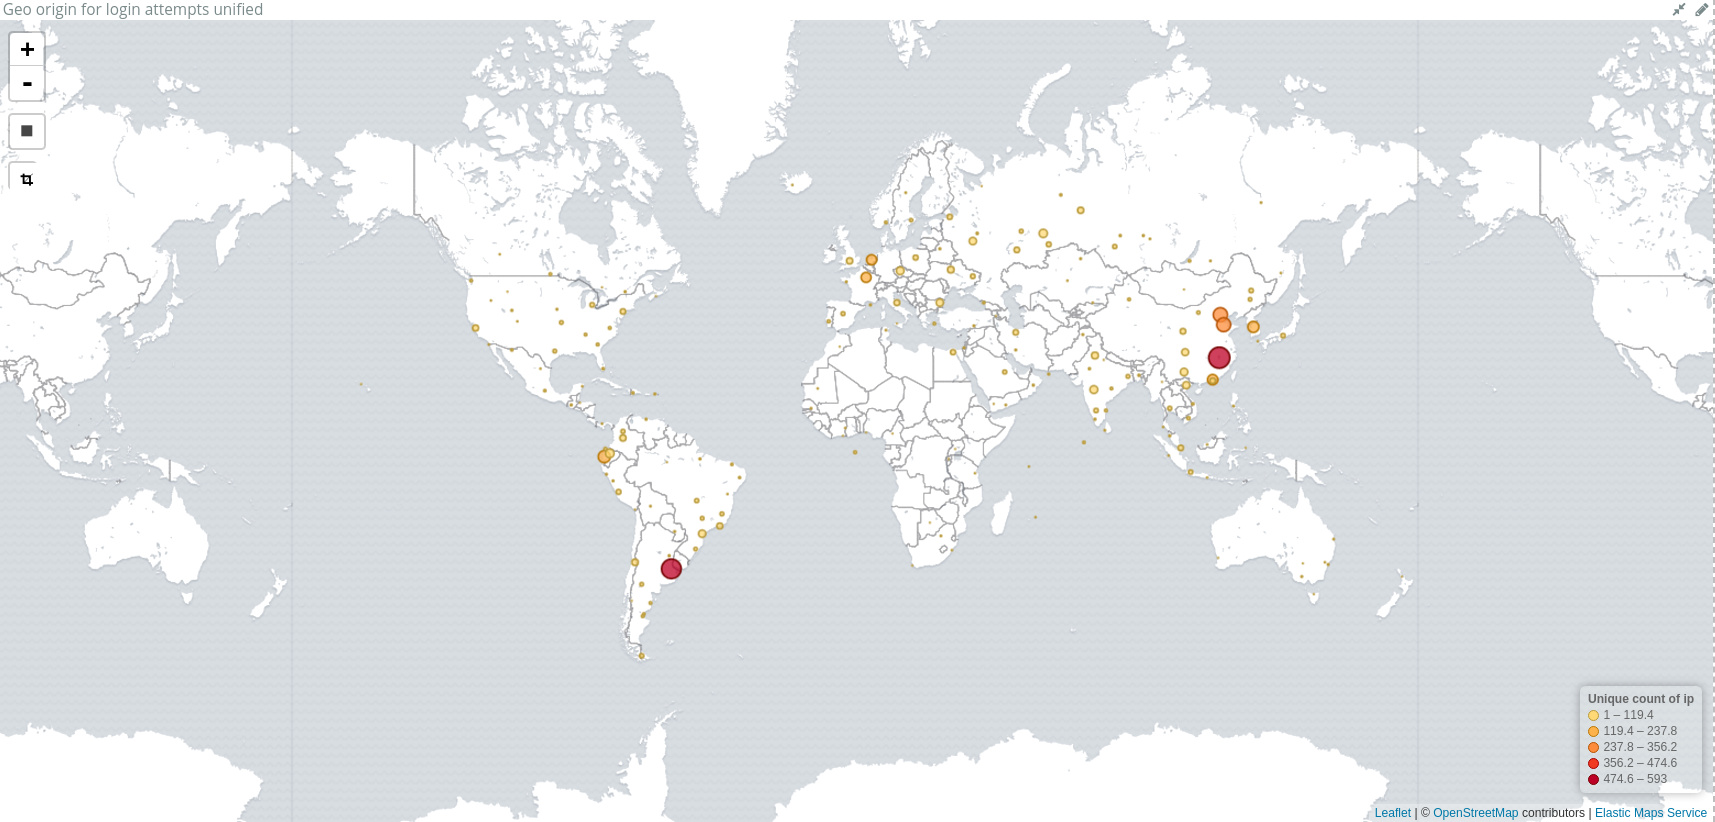
\includegraphics[scale=0.3]{images/ElasticMapUnified}
    \caption{Mapa que incluye los intentos de inicio desde la misma IP en el periodo del 4 de Junio de 2017 al 2 de Septiembre de 2017}
    \label{fig:data-map-unified}
  \end{sidewaysfigure}

  \begin{sidewaysfigure}[h]
    \centering
      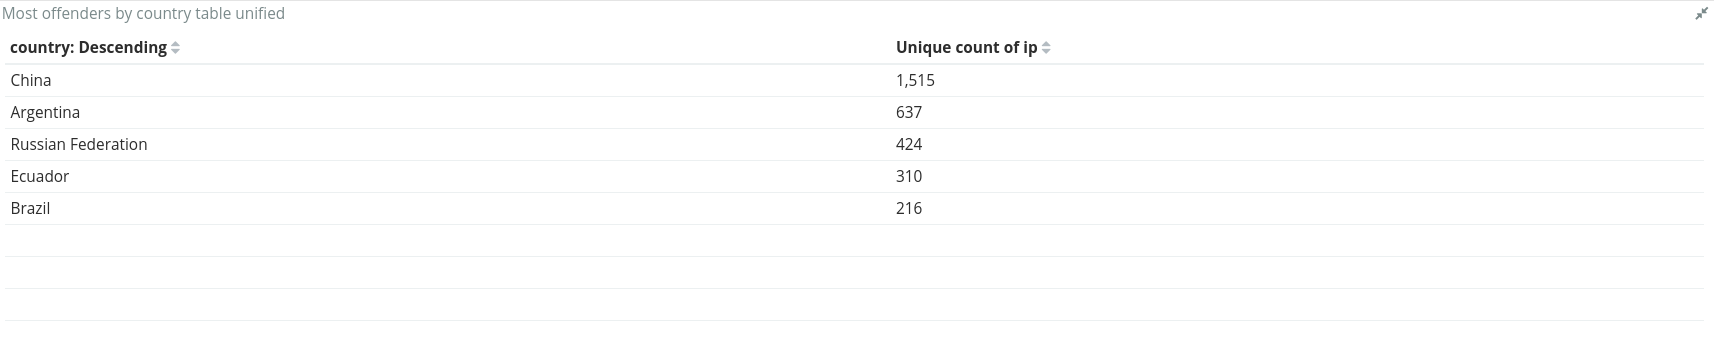
\includegraphics[scale=0.3]{images/ElasticTableByCountryUnified}
    \caption{Tabla resumen de paises que atacan más a las sondas en el periodo del 4 de Junio de 2017 al 2 de Septiembre de 2017}
    \label{fig:data-table-by-country-unified}
  \end{sidewaysfigure}

  \begin{sidewaysfigure}[h]
    \centering
      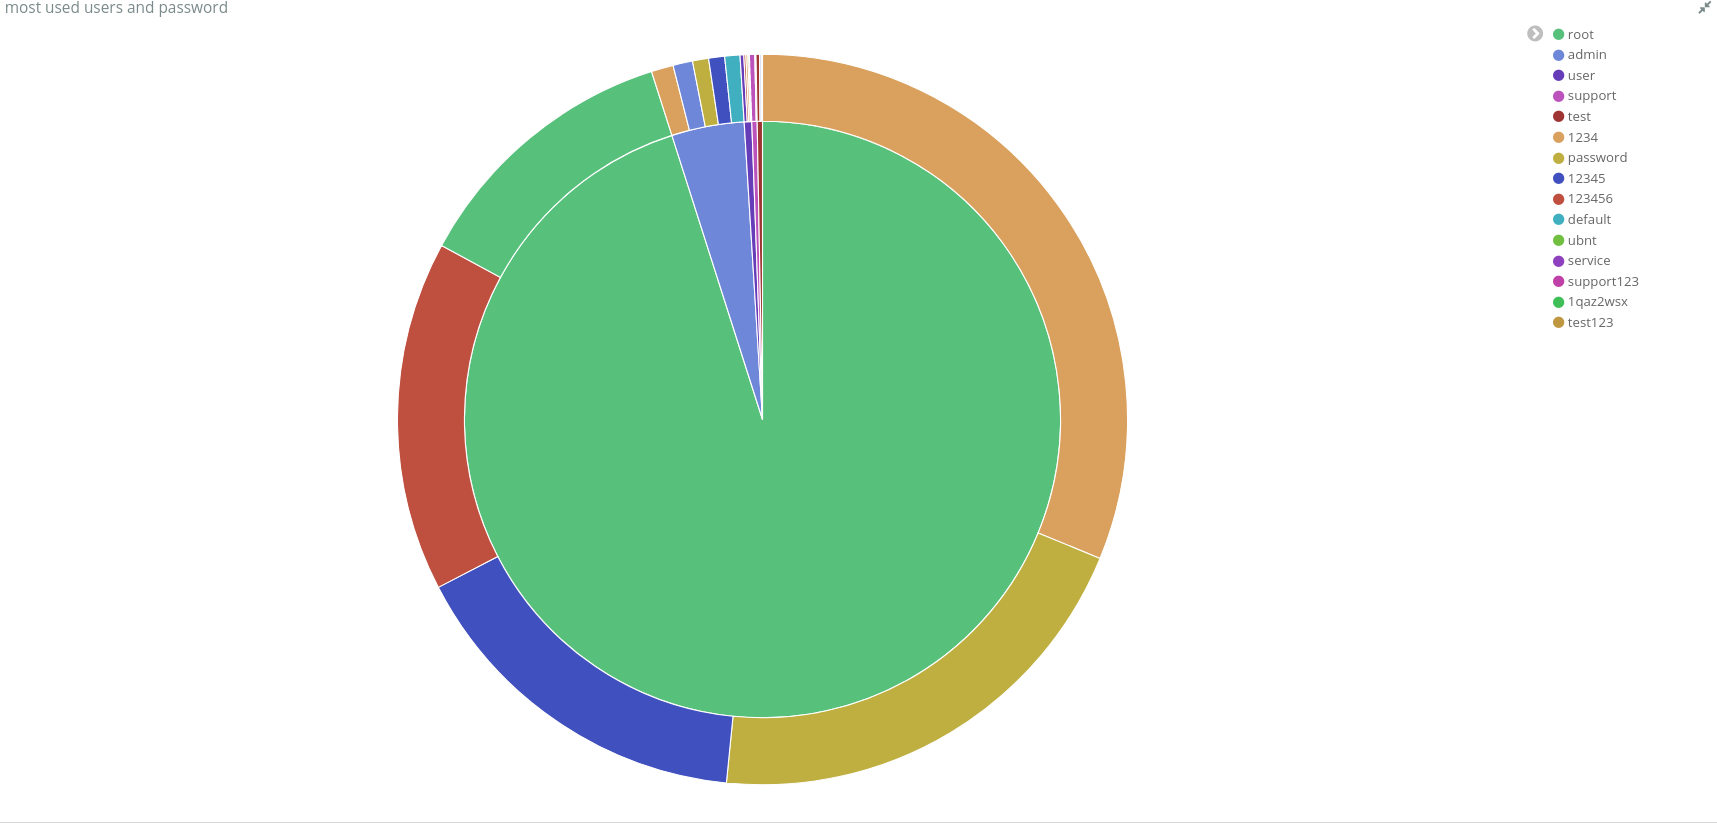
\includegraphics[scale=0.3]{images/ElasticPiePasswors}
    \caption{Contraseñas más utilizadas en los intentos de inicio de sesión en el periodo del 4 de Junio de 2017 al 2 de Septiembre de 2017}
    \label{fig:data-pie-passwords}
  \end{sidewaysfigure}

  \begin{sidewaysfigure}[h]
    \centering
      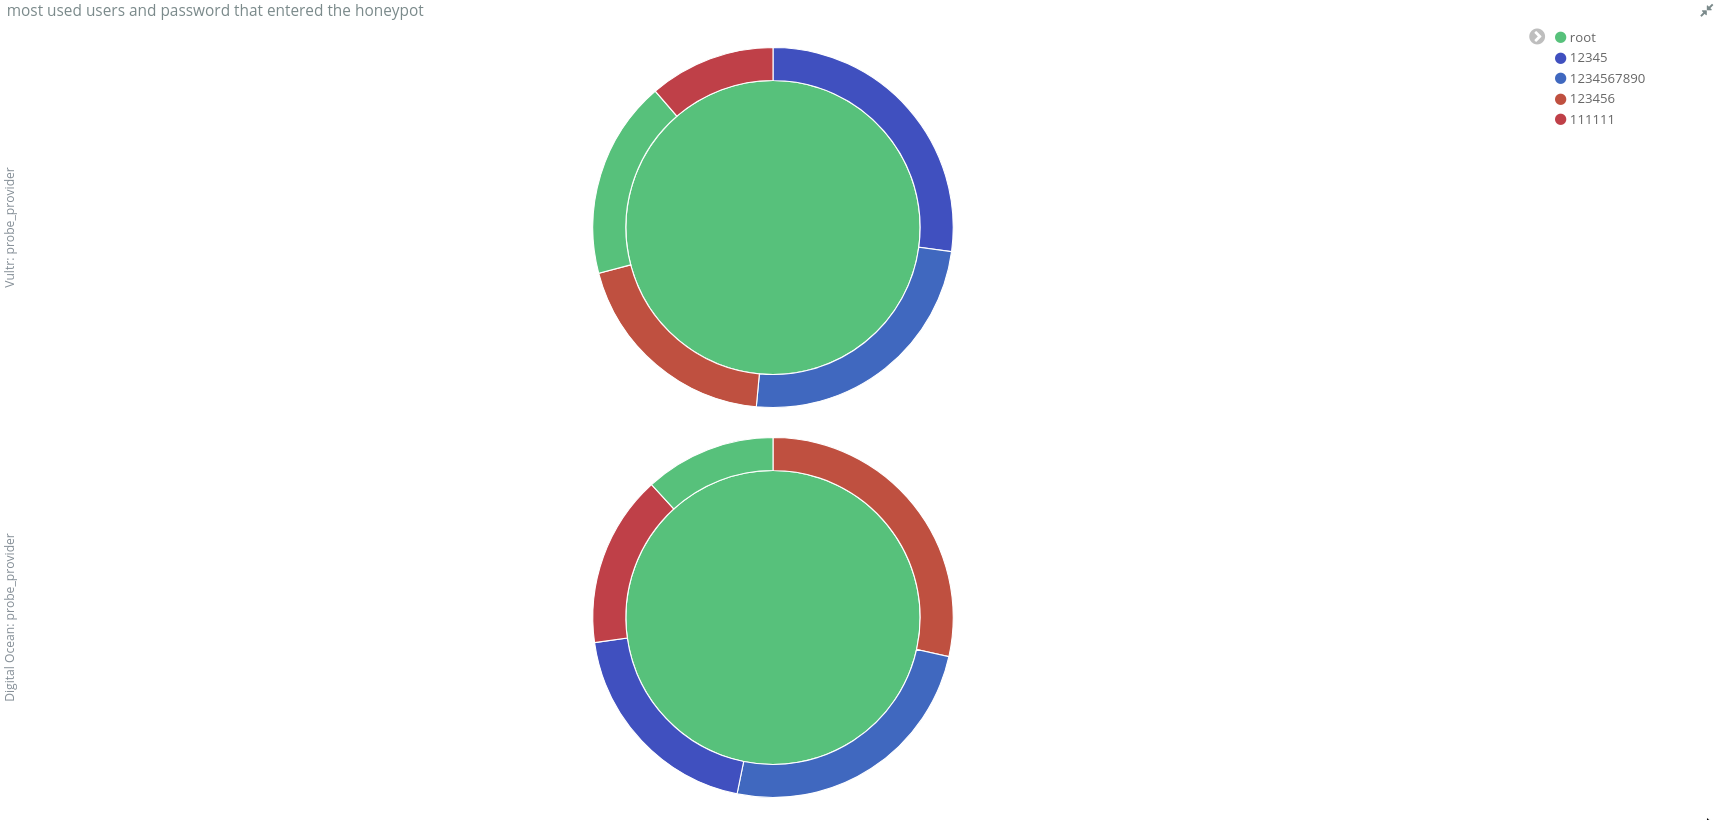
\includegraphics[scale=0.3]{images/ElasticPiePasswordSuccessful}
    \caption{Contraseñas que tuvieron éxito en los intentos de inicio de sesión en el periodo del 4 de Junio de 2017 al 2 de Septiembre de 2017}
    \label{fig:data-pie-passwords-successful}
  \end{sidewaysfigure}
  
  
  
\chapter{Trabajo futuro y conclusiones}
\section{Trabajo futuro}
\label{sec:trabajo-futuro}

De cara al trabajo futuro hay muchísimas líneas de actuación en diversas categorías. Desde mejorar la estabilidad 
y escalabilidad del sistema, aumentar el número de sondas, protocolos y sistemas operativos a exponer hasta 
mejorar la presentación de los datos mejorando la API para incluir otros formatos y una búsqueda más precisa de incidentes.

\subsubsection{Mejora de la escalabilidad de la plataforma.}

Habría que realizar un desembolso económico importante en horas de trabajo y servidores para separar los servicios expuestos
en \ref{fig:arquitectura-recolector} que son desplegados actualmente en un solo servidor. La mejora seía separar en varios servidores que creciesen
de manera horizontal atendiendo a la carga. Esto, posiblemente, involucraría el despliegue de un sistema de colas, como se analizó
en \ref{subsec:notificaciones-falco}.

El proceso de provisión y configuración también debería mejorar para acomodarse a esta nueva situación y pasar de utilizar \emph{Ansible}
en un enfoque de \emph{PhoenixServers} a imágenes inmutables con una \emph{pipeline} de \emph{CI/CD}.

\subsubsection{Extracción de ficheros en las sondas.}

Además de extraer información de las trazas sobre actividad según el protocolo, sería interesante poder extraer el contenido de disco del \emph{container}.
En nuestro caso, quizá la opción más simple para incorporar esta funcionalidad sería la de crear un registro privado de \emph{containers} y, al detectar 
una intrusión a la vez que se notifica la alerta, guardar esta versión del \emph{container} como una nueva imágen en el registro.

Luego, en la API, se podría añadir la dirección del registro privado y permitir al usuario descargar el \emph{container} para su análisis bajo su responsabilidad. 
Mantener este tipo de registros privados de \emph{containers} involucra cierta complejidad, especialmente, si la base de usuarios es elevada. Elementos como
una \emph{CDN} y almacenamiento que crece de manera dinámica serían necesarios para la supervivencia del proyecto. Desarrollar y mantener esta funcionalidad
es costoso en tiempo de desarrollo y/o en pago a terceros que ofrecen estas soluciones.

\subsubsection{Más protocolos.}

Sería interesante también ofrecer otras sondas con otros protocolos y aplicaciones (servidores web, cachés distribuídas, etc) de la que poder extraer información de otro
tipo de ataques. Añadir nuevos protocolos y sondas solo elevaría el coste económico de la partida de servidores, ya que en el estado actual del proyecto no sería 
complejo añadir nuevas sondas y protocolos.

\subsubsection{Sondas de Windows.}

Sería interesante incorporar aplicaciones \emph{Windows} en nuestro parqué de sondas. Para ello habría que analizar y construir un sistema de recolección de trazas
para \emph{Windows} al igual que se ha realizado en \ref{sec:analisis-sonda}.

Dicho análisis y desarrollo de la solución requeriría una inversión en tiempo de investigación y ejecución de varios meses y un incremento en la partida de servidores en el aspecto económico, 
pero proporcionaría información muy relevante dado que muchos sistemas criticos (hospitales, bancos, \ldots) utilizan dichos sistemas.


\subsubsection{Monetización}

Es posible la monetización del proyecto, quizás vendiendo \emph{feeds} personalizados a instituciones relevantes. Sin embargo, en el estado actual de desarrollo del proyecto
sería más fácil intentar integrar el proyecto en soluciones de inteligencia de seguridad informática ya disponibles, que ya incorporen las partes que faltan a este proyecto
(visualizaciones atractivas vía dashboard, gestión de clientes y otros \ldots).

\section{Conclusiones}

El presente proyecto en su estado actual cumple los requisitos de diseño enumerados en la sección \ref{sec:requisitos-de-disenyo}. pero, teniéndolo en cuenta, también es cierto que la potencia del modelo de \emph{honeypot} con \emph{containers} es solo explorada superficialmente en este proyecto, seria muy interesante continuar
las lineas descritas en la sección \ref{sec:trabajo-futuro} para seguir explorandolo, si se contase con la financiación adecuada.

Es además un proyecto de estas características que cubren el espectro completo (de captación a visualización) y se ha liberado su código fuente, permitiendo a terceros desarrollar sobre esta idea, algo
poco común en el area de la seguridad informática. 

Este proyecto ha sido un enorme proceso de aprendizaje personal para este autor que ha aplicado para su consecución además de conocimiento técnico, todo lo aprendido
en gestión de proyectos, gestión de expectativas y entrega continua asumidos en el mundo laboral.

\chapter{Bibliografia}

\nocite{*}
\nopagebreak
\printbibheading[title={Bibliografia},heading=none]
\printbibliography[title={Referencias},heading=none]
\nopagebreak

\section*{Definiciones y abreviaturas}

\begin{itemize}
    \item[\textbf{API}] \emph{Application program interface}. interfaz desarrollada para ser utilizada por \emph{software} y no directamente para humanos.
    \item[\textbf{LTS}] \emph{Long Term Support}. Una distribución de \emph{software} en la que se actualiza y mantiene aunque se hayan publicado nuevas versiones del \emph{software}.
    \item[\textbf{CLI}] \emph{Command Line Interface}. Método que permite a los usuarios dar instrucciones a algún programa informático por medio de una línea de texto simple
    \item[\textbf{XML}] \emph{eXtensible Markup Language}. Traducido como \emph{Lenguaje de Marcado Extensible} o \emph{Lenguaje de Marcas Extensible}, es un meta-lenguaje que permite definir lenguajes de marcas desarrollado por el World Wide Web Consortium (W3C) utilizado para almacenar datos en forma legible.
    \item[\textbf{JSON}] \emph{Javascript Object Notation}. es un formato de representación de datos, alternativa a XML.
    \item[\textbf{pipeline}] Es una cadena de elementos que procesan o generan algo de manera que el elemento siguiente utiliza el resultado del paso anterior.
    \item[\textbf{CI}] \emph{Continuous Integration}. Es una \emph{pipeline} cuyo objetivo es la de crear un artefacto \emph{software} tras cada cambio en el sistema de control de versiones.
    \item[\textbf{CD}] \emph{Continuous Delivery}. Es una \emph{pipeline} que además de realizar las funciones de CI, se encarga del despliegue a producción del artefacto generado. 
    \item[\textbf{honeypot}] o sistema trampa o señuelo, es una herramienta de la seguridad informática dispuesto en una red o sistema informático para ser el objetivo de un posible ataque informático, y así poder detectarlo y obtener información del mismo y del atacante.
    \item[\textbf{kernel}] Núcleo del sistema, cuando hablamos del \emph{kernel} en este proyecto nos referimos normalmente al \emph{kernel} de un sistema GNU/Linux. 
    \item[\textbf{container}] Proceso del sistema que tiene asociado un \emph{namespace}, un \emph{cgroup} y cierto acceso a funciones del \emph{kernel} que permite virtualizar un sistema a nivel de sistema operativo. 
    \item[\textbf{namespace}] Mecanismo mediante el kernel limita la visualización del sistema total o parcialmente a un proceso, así un proceso X en un \emph{namespace} N podrá visualizar o no
    dispositivos de red, lista de procesos, discos duros \ldots (véase \cite{wiki-namespaces}).
    \item[\textbf{cgroup}] Mecanismo mediante el kernel limita la cantidad de recursos de CPU, RAM y operaciones de entrada/salida que un proceso puede realizar. (véase \cite{wiki-cgroups})
\end{itemize}




    



%%% Local Variables: 
%%% mode: latex
%%% TeX-master: "main"
%%% End:
